%%%% Шаблон Отчета по практике <<SPbPU-student-thesis-template>>  %%%%
%%
%%   Создан на основе глубокой переработки шаблона российских кандидатских и докторских диссертаций [1]. 
%%   
%%   Полный список различий может быть получен командами git.
%%   Лист авторов-составителей расположен в README.md файле.
%%   Подробные инструкции по использованию в [1,2].
%%   
%%   Рекомендуем установить TeX Live + TeXstudio
%%   <<Стандартная>> компиляция 2-3 РАЗА с помощью pdflatex + biber (для библиографии)     
%%  
%%%% Student thesis template <<SPbPU-student-thesis-template>> %%%%
%%
%%   Created on the basis of deep modifification of the Russian candidate and doctorate thesis template [1]. 
%%   
%%   Full list of differences can be achieved by git commands.
%%   List of template authors can be seen in the README.md file.
%%   Detailed instructions of usage, see, please in [1,2].
%%     
%%   [1] github.com/AndreyAkinshin/Russian-Phd-LaTeX-Dissertation-Template 
%%   [2] Author_guide_SPBPU-student-thesis-template.pdf
%%   
%%   It is recommended to install TeX Live + TeXstudio   
%%   Default compilation 2-3 TIMES with pdflatex + biber (for the bibliography)
%%  
%%%% Preamble start %%%%  
%%
%%   Please, do not modify files in the preamble
%%
\newcommand*{\anyptfilebase}{template_settings/bpfont} 
\newcommand*{\anyptsize}{14} 		 
\RequirePackage[l2tabu,orthodox]{nag} 
\documentclass[extrafontsizes,a4paper,*pt,oneside,openany]{memoir}
%% Режим черновика
\makeatletter
\@ifundefined{c@draft}{
  \newcounter{draft}
  \setcounter{draft}{0}  % 0 --- чистовик (максимальное соблюдение ГОСТ)
                         % 1 --- черновик (отклонения от ГОСТ, но быстрая сборка итоговых PDF)
}{}
\makeatother

%% Библиография

%% Внимание! При использовании bibtex8 необходимо удалить все
%% цитирования из  ../common/characteristic.tex
\newcounter{bibliosel}
\setcounter{bibliosel}{1}           % 0 --- встроенная реализация с загрузкой файла через движок bibtex8; 1 --- реализация пакетом biblatex через движок biber

               
%%% Проверка используемого TeX-движка %%%
\usepackage{iftex}[2013/04/04]
\newif\ifxetexorluatex   % определяем новый условный оператор (http://tex.stackexchange.com/a/47579/79756)
\ifXeTeX
    \xetexorluatextrue
\else
    \ifLuaTeX
        \xetexorluatextrue
    \else
        \xetexorluatexfalse
    \fi
\fi

\RequirePackage{etoolbox}[2015/08/02]               % Для продвинутой проверки разных условий

%%% Поля и разметка страницы %%%

\usepackage{pdflscape}                              % Для включения альбомных страниц
\usepackage{geometry}                               % Для последующего задания полей

%%% Математические пакеты %%%
\usepackage{amsfonts,amsmath,amssymb,amscd,amsthm}  % Математические дополнения от AMS
% %amsthm should be loaded after amsmath!!

\usepackage{mathtools}                              % Добавляет окружение multlined

%%%% Установки для размера шрифта 14 pt %%%%
%% Формирование переменных и констант для сравнения (один раз для всех подключаемых файлов)%%
%% должно располагаться до вызова пакета fontspec или polyglossia, потому что они сбивают его работу
\newlength{\curtextsize}
\newlength{\bigtextsize}
\setlength{\bigtextsize}{13.9pt}

\makeatletter
%\show\f@size                                       % неплохо для отслеживания, но вызывает стопорение процесса, если документ компилируется без команды  -interaction=nonstopmode 
\setlength{\curtextsize}{\f@size pt}
\makeatother

%%% Кодировки и шрифты %%%
\ifxetexorluatex
    \usepackage{polyglossia}[2014/05/21]            % Поддержка многоязычности (fontspec подгружается автоматически)
\else
    \RequirePDFTeX                                  % tests for PDFTEX use and throws an error if a different engine is being used
   %%% Решение проблемы копирования текста в буфер кракозябрами
%    \input glyphtounicode.tex
%    \input glyphtounicode-cmr.tex %from pdfx package
%    \pdfgentounicode=1
    \usepackage{cmap}                               % Улучшенный поиск русских слов в полученном pdf-файле
    \defaulthyphenchar=127                          % Если стоит до fontenc, то переносы не впишутся в выделяемый текст при копировании его в буфер обмена
    
%    \usepackage[T2A]{fontenc}                       % Поддержка русских букв
    \usepackage[T2A,T1]{fontenc}
    \usepackage[utf8]{inputenc}[2014/04/30]         % Кодировка utf8
    \usepackage[english, russian]{babel}[2014/03/24]% Языки: русский, английский
\fi
\usepackage{tempora} %TemporaLGCUni of Times type
\usepackage{newtxmath} %math font of Times type
% need to set the monospace=typewritter font
%https://tex.stackexchange.com/questions/213835/using-many-typewriter-fonts-in-a-single-document

\makeatletter %load fonts for cmtt
\providecommand{\EC@ttfamily}[5]{%
	\DeclareFontShape{#1}{#2}{#3}{#4}{
		<-8.5>#50800
		<8.5-9.5>#50900
		<9.5-10.5>#51000
		<10.5-11.5>#51095
		<11.5-13>#51200
		<13-15.5>#51440
		<15.5-18.5>#51728
		<18.5-22>#52074
		<22-27>#52488
		<27-32>#52986
		<32->#53583}{}}
\DeclareFontFamily{T1}{cmtt}{}
\DeclareFontFamily{T2A}{cmtt}{}
\EC@ttfamily{T1}{cmtt}{m}{n}{ectt}
\EC@ttfamily{T1}{cmtt}{m}{sl}{ecst}
\EC@ttfamily{T1}{cmtt}{m}{it}{ecit}
\EC@ttfamily{T1}{cmtt}{m}{sc}{ectc}
\DeclareFontShape{T1}{cmtt}{bx}{n}%
{<->ssub*cmtt/m/n}{}
\DeclareFontShape{T1}{cmtt}{bx}{it}%
{<->ssub*cmtt/m/it}{}
\EC@ttfamily{T2A}{cmtt}{m}{n}{latt}
\EC@ttfamily{T2A}{cmtt}{m}{sl}{last}
\EC@ttfamily{T2A}{cmtt}{m}{it}{lait}
\EC@ttfamily{T2A}{cmtt}{m}{sc}{latc}
\DeclareFontShape{T2A}{cmtt}{bx}{n}%
{<->ssub*cmtt/m/n}{}
\DeclareFontShape{T2A}{cmtt}{bx}{it}%
{<->ssub*cmtt/m/it}{}
\makeatletter

%\makeatletter %load fonts for cmtt
%\providecommand{\EC@ttfamily}[5]{%
%	\DeclareFontShape{#1}{#2}{#3}{#4}{
%		<-8.5>#50800
%		<8.5-9.5>#50900
%		<9.5-10.5>#51000
%		<10.5-11.5>#51095
%		<11.5-13>#51200
%		<13-15.5>#51440
%		<15.5-18.5>#51728
%		<18.5-22>#52074
%		<22-27>#52488
%		<27-32>#52986
%		<32->#53583}{}}
%\DeclareFontFamily{T2A}{cmtt}{\hyphenchar\font\m@ne}
%\EC@ttfamily{T2A}{cmtt}{m}{n}{latt}
%\EC@ttfamily{T2A}{cmtt}{m}{sl}{last}
%\EC@ttfamily{T2A}{cmtt}{m}{it}{lait}
%\EC@ttfamily{T2A}{cmtt}{m}{sc}{latc}
%\DeclareFontShape{T2A}{cmtt}{bx}{n}%
%{<->ssub*cmtt/m/n}{}
%\DeclareFontShape{T2A}{cmtt}{bx}{it}%
%{<->ssub*cmtt/m/it}{}
%\makeatletter

%\makeatletter
%\input{t1lmtt.fd}
%\@namedef{T1+lmtt}{}
%\makeatother


\renewcommand{\ttdefault}{cmtt}
%\renewcommand{\ttdefault}{lcmtt} %покрупнее
%\usepackage[scaled=.85]{DejaVuSansMono} %слишком похож на рубленый
%\newfont{\wasyten}{wasy10} %название команды для вызова / название шрифта



%Другие шрифты:
% математика
%\usepackage[lite]{mtpro2}
%https://pctex.com/mtpro2.html
% текст        
% https://www.ctan.org/pkg/paratype
%       \usepackage[scaled=0.925]{XCharter}[2017/06/25] % Подключение русифицированных шрифтов XCharter
%\usepackage{pscyr}
%    \IfFileExists{pscyr.sty}{}{}  % Красивые русские шрифты
%\fi

%https://tex.stackexchange.com/questions/8260/what-are-the-various-units-ex-em-in-pt-bp-dd-pc-expressed-in-mm
\usepackage{printlen} %для измерения и вывода параменторов шрифтов, отступов, интервалов

\usepackage{bm} %для жирных начертаний символов

\usepackage{csquotes} %to check quotes

%%% Оформление абзацев %%%
\usepackage{indentfirst}                            % Красная строка

%%% Цвета %%%
%\usepackage[dvipsnames,usenames]{color}
\usepackage{colortbl}
\usepackage[dvipsnames, table, hyperref, cmyk]{xcolor} % Вероятно, более новый вариант, вместо предыдущих двух строк. Конвертация всех цветов в cmyk заложена как удовлетворение возможного требования типографий. Возможно конвертирование и в rgb.

%%% Таблицы %%%
\usepackage{longtable}                              % Длинные таблицы
\usepackage{multirow,makecell}                      % Улучшенное форматирование таблиц:
													% multirow - строки на несколько ячеек, 
												
													% makecell - сесколько строк в ячейке.
													% не работает, если внутри, например, \verb|text| -> \texttt{text}
													% аналоги
%https://tex.stackexchange.com/questions/2441/how-to-add-a-forced-line-break-inside-a-table-cell								
						
													

%%% Общее форматирование
%\usepackage{soul} % используется ulem
\usepackage{soulutf8}                               % Поддержка переносоустойчивых подчёркиваний и зачёркиваний
\usepackage{icomma}                                 % Запятая в десятичных дробях



%%% Предметный указатель  ГОСТ 7.78-99 Index %%%
%c обобщенными рубриками или развернутый
%или указатель терминов (в общем случае - произвольное число указателей)
%подключать до hyperref

%\usepackage{makeidx} %возможно, необходимо подключить И/ИЛИ пройти Tools-> Commands -> MakeIndex

\usepackage{imakeidx} 
%\indexsetup{level=\section*,toclevel=section,noclearpage}
\makeindex[program=makeindex,
options=-s template_settings/common/myindex.ist, %подключаем стилевой файл для форматирования вывода
name=ru, % префикс для русских указателей 
% если убрать <<ru>>, то для работы дефолтового придется вручную включать Tools-> Commands -> MakeIndex
title={\chapterLight{} 
%   \hrule{}
	Предметный указатель
%	\hrule{}
} 
%,columns=1 %по умолчанию 2
]
\makeindex[program=makeindex,
options=-s template_settings/common/myindex.ist, %подключаем стилевой файл для форматирования вывода
name=en, % префикс для английских указателей
title={\chapterLight{}
%	\hrule{}
	Index
%	\hrule{}
} 
%,columns=1 %по умолчанию 2
] 
%убрать добавление <<title>> в содержание:
%\noindexintoc %not to add index title in PURE makeidx %intoc is false by default with imakeidx


%       https://tex.stackexchange.com/a/132415/44348
%\makeatletter
%% we want hyphenation also in the first word
\renewcommand{\@idxitem}{\par\hangindent40\p@\hspace{0pt}\ignorespaces}
%% we don't want a page break before a subitem %implemented in the previous one
%%\renewcommand\subitem{\@idxitem\nobreak\hspace*{20\p@}}
%\makeatother


%%% Фиксация плавающих объектов





%%% Гиперссылки %%%
\usepackage{hyperref}[2012/11/06]

%%% Изображения %%%
\usepackage{graphicx}[2014/04/25]                   % Подключаем пакет работы с графикой

%%% Списки %%%
\usepackage[shortlabels]{enumitem} % shortlabels для того, чтобы изменять токены в списках с дефолтных (иерархическая структура) на произвольныею

%%% Подписи %%%
\usepackage{caption}[2013/05/02]                    % Для управления подписями (рисунков и таблиц) % Может управлять номерами рисунков и таблиц с caption %Иногда может управлять заголовками в списках рисунков и таблиц


\usepackage{subcaption}[2013/02/03]                 % Работа с подрисунками и подобным

%%% Счётчики %%%
%\usepackage[figure,table]{totalcount}               % Счётчик рисунков и таблиц. Взамен используется xassoccnt 
\usepackage{totcount}                               % Пакет создания счётчиков на основе последнего номера подсчитываемого элемента (может требовать дважды компилировать документ)
\usepackage{totpages}                               % Счётчик страниц, совместимый с hyperref (ссылается на номер последней страницы). Желательно ставить последним пакетом в преамбуле

\usepackage{xassoccnt} % для подсчета сумм приложений, рисунков, таблиц 


%%% Продвинутое управление групповыми ссылками (пока только формулами) %%%
\ifxetexorluatex
    \usepackage{cleveref}                           % cleveref корректно считывает язык из настроек polyglossia
\else
    \usepackage[russian]{cleveref}                  % cleveref имеет сложности со считыванием языка из babel. Такое решение русификации вывода выбрано вместо определения в documentclass из опасности что-то лишнее передать во все остальные пакеты, включая библиографию.
\fi
\creflabelformat{equation}{#2#1#3}                  % Формат по умолчанию ставил круглые скобки вокруг каждого номера ссылки, теперь просто номера ссылок без какого-либо дополнительного оформления



\ifnumequal{\value{draft}}{1}{% Черновик
    \usepackage[firstpage]{draftwatermark}
    \SetWatermarkText{DRAFT}
    \SetWatermarkFontSize{14pt}
    \SetWatermarkScale{15}
    \SetWatermarkAngle{45}
}{}

  
%%% Прикладные пакеты %%% 
%\usepackage{calc}               % Пакет для расчётов параметров, например длины

%%% Для добавления Стр. над номерами страниц в оглавлении
%%% http://tex.stackexchange.com/a/306950
\usepackage{afterpage}

\urlstyle{rm} % links in Times


%\makeatletter
%%расстояние после ToC title до 1ой строчки 
%%для достижения одинаковых отсупов переопределено формирование базового ToC
%\renewcommand{\aftertoctitle}{\par\nobreak\vskip1\curtextsize}
%\makeatother

%https://tex.stackexchange.com/questions/170912/contents-page-in-two-different-languages
%\makeatletter
\newcommand\russiantableofcontents{%
%	\if@twocolumn
%	\@restonecoltrue\onecolumn
%	\else
%	\@restonecolfalse
%	\fi
	%  \begin{otherlanguage}{russian}
	\chapter*{%
	\normalfont\MakeUppercase{Содержание} %слово <<Содержание>> в стилю chaperLight, по факту убираем \bfseries
%		    \contentsname
%		    \@mkboth{\MakeUppercaseСодержание}
%		            {\MakeUppercaseСодержание}%
	}%
%\hrule
\vspace*{-1\curtextsize} %убрать лишний отступ в таблице
	\@starttoc{tuc}%
	%  \end{otherlanguage}
%	\if@restonecol\twocolumn\fi
}
\newcommand{\addtocru}[2]{%
	\addcontentsline{tuc}{#1}{\protect\numberline{\csname the#1\endcsname}#2}%
%	\addcontentsline{tuc}{#1}{#2}%
}
\newcommand{\addtocruNoProtect}[2]{%
%	\addcontentsline{tuc}{#1}{\protect\numberline{\csname the#1\endcsname}#2}%
		\addcontentsline{tuc}{#1}{#2}%
}

%обеспечение красивого порядка вывода содержаний и названий разделов, подразделов и т.п.
\newcommand\englishtableofcontents{%
	%	\if@twocolumn
	%	\@restonecoltrue\onecolumn
	%	\else
	%	\@restonecolfalse
	%	\fi
	%  \begin{otherlanguage}{russian}
	\chapter*{%
		\normalfont\MakeUppercase{Content} %слово <<Содержание>> в стилю chaperLight, по факту убираем \bfseries
		%		    \contentsname
		%		    \@mkboth{\MakeUppercaseСодержание}
		%		            {\MakeUppercaseСодержание}%
	}%
	%\hrule
	\vspace*{-1\curtextsize} %убрать лишний отступ в таблице
	\@starttoc{tec}%
	%  \end{otherlanguage}
	%	\if@restonecol\twocolumn\fi
}
\newcommand{\addtocen}[2]{%
		\addcontentsline{tec}{#1}{\protect\numberline{\csname the#1\endcsname}#2}%
%	\addcontentsline{tec}{#1}{#2}%
}
\newcommand{\addtocenNoProtect}[2]{%for preface, introduction etc
%	\addcontentsline{tec}{#1}{\protect\numberline{\csname the#1\endcsname}#2}%
		\addcontentsline{tec}{#1}{#2}%
}


%стандартный вывод в toc можно использовать, если издание только на английском или русском.
%переопределена, чтобы обеспечить одинаковые отсупы от названия ToC (toc, tec, tuc) до первой строки
\renewcommand\tableofcontents{%
	%	\if@twocolumn
	%	\@restonecoltrue\onecolumn
	%	\else
	%	\@restonecolfalse
	%	\fi
	%  \begin{otherlanguage}{russian}
	\chapter*{%
		\MakeUppercase{Содержание} %слово <<Содержание>> 
		%		    \contentsname
		%		    \@mkboth{\MakeUppercaseСодержание}
		%		            {\MakeUppercaseСодержание}%
	}%
	%\hrule
%	\vspace*{-0.58\curtextsize} %убрать/добавить отступ от таблицы
	\@starttoc{toc}%
	%  \end{otherlanguage}
	%	\if@restonecol\twocolumn\fi
}
\newcommand{\addetoc}[2]{%
		\addcontentsline{toc}{#1}{\protect\numberline{\csname the#1\endcsname}#2}%
}
%\newcommand{\addtocru}[2]{%
%	\addcontentsline{tuc}{#1}{\protect\numberline{\csname the#1\endcsname}#2}%
%	%	\addcontentsline{tuc}{#1}{#2}%
%}

%\makeatother

%http://latex.org/forum/viewtopic.php?t=5438         
\usepackage{tabularx}

%%https://tex.stackexchange.com/a/362229
\usepackage{datatool-base}
\usepackage{mfirstuc} %первая буква прописная

\usepackage{layouts}

\newenvironment{abstr}{\smallA\itshape}{\normalfont\normalsize}


\usepackage[normalem]{ulem} % для перечеркнутых сроков команда \sout{text}
\newcommand{\soutthick}[1]{%
	\renewcommand{\ULthickness}{2.4pt}%
	\sout{#1}%
	\renewcommand{\ULthickness}{.4pt}% Resetting to ulem default
}

%для подчёркнутых команд
%https://tex.stackexchange.com/questions/270286/uline-not-work-for-command-arguments
\useunder{\uline}{\ulined}{}

\usepackage{environ} % for Uppercase in Keywords
%https://tex.stackexchange.com/questions/249628/uppercase-whole-newenvironment
% недостаток - новые окружения не подхватываются TexStudio

\usepackage{textcase} % for \MakeTextUppercase

%for svg pictures
%\usepackage{svg}


%%% Mailto %%% 
%%%https://tex.stackexchange.com/questions/128424/how-to-create-email-hyperlink-with-predefined-subject-in-latex
%% unfortunatelly Adobe does not handle Recipient name + email, e.g.
%% Vladimir Parkhomenko<parhomenko.v@gmail.com>


%mailto with subject (impossible with href)
%mailto anybody without email body
\makeatletter
\newcommand\mailtoab[3]{%                %\newcommand\tpj@compose@mailto[3]{%
	\edef\@tempa{mailto:#1?subject=#2 }%
	\edef\@tempb{\expandafter\html@spaces\@tempa\@empty}%
	\href{\@tempb}{#3}}
\catcode\%=11
\def\html@spaces#1 #2{#1%20\ifx#2\@empty\else\expandafter\html@spaces\fi#2}
	\catcode\%=14
	\makeatother
	
	
	%${email}{Subject}{email start body}{text in pdf}
	\makeatletter
	\newcommand\mailto[4]{%                %\newcommand\tpj@compose@mailto[3]{%
		\edef\@tempa{mailto:#1?subject=#2\&body=#3 }%
		\edef\@tempb{\expandafter\html@spaces\@tempa\@empty}%
		\href{\@tempb}{#4}}
	%% with %20 instead of spaces
	%\catcode\%=11
	%\def\html@spaces#1 #2{#1%20\ifx#2\@empty\else\expandafter\html@spaces\fi#2}
	%\catcode\%=14
	\makeatother
	
	%% MLABSED 2017 author
	%%${email}{Subject}{email start body}{text in pdf}
	\makeatletter
	\newcommand\mailtoMLABSEDauthor[3]{%                
		\edef\@tempa{mailto:#1?subject=MLABSED 2017\&body=#2 }%
		\edef\@tempb{\expandafter\html@spaces\@tempa\@empty}%
		\href{\@tempb}{#3}}
	%% with %20 instead of spaces
	%\catcode\%=11
	%\def\html@spaces#1 #2{#1%20\ifx#2\@empty\else\expandafter\html@spaces\fi#2}
	%\catcode\%=14
	\makeatother
	
	
	%%Vladimir Parkhomenko
	\makeatletter
	\newcommand\mailtopa[1]{%                %\newcommand\tpj@compose@mailto[3]{%
		\edef\@tempa{mailto:parhomenko.v@gmail.com?subject=#1\&body=Dear Vladimir, }%
		\edef\@tempb{\expandafter\html@spaces\@tempa\@empty}%
		\href{\@tempb}{Vladimir.Parkhomenko@spbstu.ru}}
	\catcode\%=11
	\def\html@spaces#1 #2{#1%20\ifx#2\@empty\else\expandafter\html@spaces\fi#2}
		\catcode\%=14
		\makeatother
		
		%%Alexey Buzmakov
		\makeatletter
		\newcommand\mailtobu[1]{%                %\newcommand\tpj@compose@mailto[3]{%
			\edef\@tempa{mailto:abuzmakov@gmail.com?subject=#1\&body=Dear Alexey, }%
			\edef\@tempb{\expandafter\html@spaces\@tempa\@empty}%
			\href{\@tempb}{abuzmakov@gmail.com}}
		\catcode\%=11
		\def\html@spaces#1 #2{#1%20\ifx#2\@empty\else\expandafter\html@spaces\fi#2}
			\catcode\%=14
			\makeatother
			
			%%Xenia Naidenova
			\makeatletter
			\newcommand\mailtona[1]{%                %\newcommand\tpj@compose@mailto[3]{%
				\edef\@tempa{mailto:ksennaidd@gmail.com?subject=#1\&body=Dear Xenia, }%
				\edef\@tempb{\expandafter\html@spaces\@tempa\@empty}%
				\href{\@tempb}{ksennaidd@gmail.com}}
			\catcode\%=11
			\def\html@spaces#1 #2{#1%20\ifx#2\@empty\else\expandafter\html@spaces\fi#2}
				\catcode\%=14
				\makeatother
				
				
				%%Konstantin Shvetsov
				\makeatletter
				\newcommand\mailtosh[1]{%                %\newcommand\tpj@compose@mailto[3]{%
					\edef\@tempa{mailto:shvetsov@inbox.ru?subject=#1\&body=Dear Konstantin, }%
					\edef\@tempb{\expandafter\html@spaces\@tempa\@empty}%
					\href{\@tempb}{Konstantin.Shvetsov@spbstu.ru}}
				\catcode\%=11
				\def\html@spaces#1 #2{#1%20\ifx#2\@empty\else\expandafter\html@spaces\fi#2}
					\catcode\%=14
					\makeatother


\usepackage{tabu, tabulary}  %таблицы с автоматически подбирающейся шириной столбцов
\usepackage{fr-longtable}    %ради \endlasthead

% Листинги с исходным кодом программ
\usepackage{fancyvrb}
\usepackage{listings}
\lccode`\~=0\relax %Без этого хака из-за особенностей пакета listings перестают работать конструкции с \MakeLowercase и т. п. в (xe|lua)latex

% Русская традиция начертания греческих букв
\usepackage{upgreek} % прямые греческие ради русской традиции

%https://tex.stackexchange.com/a/62351/44348
% Микротипографика
\ifnumequal{\value{draft}}{0}{% Только если у нас режим чистовика
    \usepackage[final,letterspace=150]{microtype}[2016/05/14] % улучшает представление букв и слов в строках, может помочь при наличии отдельно висящих слов
%    \lsstyle for letterspace style of letters
}{}

% Отметка о версии черновика на каждой странице
% Чтобы работало надо в своей локальной копии по инструкции
% https://www.ctan.org/pkg/gitinfo2 создать небходимые файлы в папке
% ./git/hooks
% If you’re familiar with tweaking git, you can probably work it out for
% yourself. If not, I suggest you follow these steps:
% 1. First, you need a git repository and working tree. For this example,
% let’s suppose that the root of the working tree is in ~/compsci
% 2. Copy the file post-xxx-sample.txt (which is in the same folder of
% your TEX distribution as this pdf) into the git hooks directory in your
% working copy. In our example case, you should end up with a file called
% ~/compsci/.git/hooks/post-checkout
% 3. If you’re using a unix-like system, don’t forget to make the file executable.
% Just how you do this is outside the scope of this manual, but one
% possible way is with commands such as this:
% chmod g+x post-checkout.
% 4. Test your setup with “git checkout master” (or another suitable branch
% name). This should generate copies of gitHeadInfo.gin in the directories
% you intended.
% 5. Now make two more copies of this file in the same directory (hooks),
% calling them post-commit and post-merge, and you’re done. As before,
% users of unix-like systems should ensure these files are marked as
% executable.
\ifnumequal{\value{draft}}{1}{% Черновик
   \IfFileExists{.git/gitHeadInfo.gin}{                                        
      \usepackage[mark,pcount]{gitinfo2}
      \renewcommand{\gitMark}{rev.\gitAbbrevHash\quad\gitCommitterEmail\quad\gitAuthorIsoDate}
      \renewcommand{\gitMarkFormat}{\color{Gray}\small\bfseries}
   }{}
}{}         
%%%%%%%%%%%%%%%%%%%%%%%%%%%%%%%%%%%%%%%%%%%%%%%%%%%%%%
%%%% Файл упрощённых настроек шаблона диссертации %%%%
%%%%%%%%%%%%%%%%%%%%%%%%%%%%%%%%%%%%%%%%%%%%%%%%%%%%%%

%%% Инициализирование переменных, не трогать!  %%%
\newcounter{intvl}
\newcounter{otstup}
\newcounter{contnumeq}
\newcounter{contnumfig}
\newcounter{contnumtab}
\newcounter{pgnum}
\newcounter{chapstyle}
\newcounter{headingdelim}
\newcounter{headingalign}
\newcounter{headingsize}
\newcounter{tabcap}
\newcounter{tablaba}
\newcounter{tabtita}
\newcounter{docType} 		% тип документа
\newcounter{tskPrint} 		% печать Задания на ВКР двух(одно)сторонняя
\newcounter{tskPages}       % для учёта количества страниц в Задании
\newcounter{tskPageFirst}   % для учёта количества страниц в Задании
\newcounter{tskPageLast}    % для учёта количества страниц в Задании 
\newcounter{sumPrint} 		% печать Реферата на ВКР двух(одно)сторонняя
\newcounter{sumPages}       % для учёта количества страниц в Реферате
\newcounter{sumPageFirst}   % для учёта количества страниц в Реферате
\newcounter{sumPageLast}    % для учёта количества страниц в Реферате 
\newcommand{\Single}{0.78}  % пропорция для одинароного отступа в \Spacing
%%%%%%%%%%%%%%%%%%%%%%%%%%%%%%%%%%%%%%%%%%%%%%%%%%

%%% Область упрощённого управления оформлением %%%

% Управление перенесено в главые файлы компиляции ВКР, Задания, Реферата
\setcounter{tskPrint}{0} %по умолчанию односторонняя печать              
%\setcounter{sumPrint}{0} %по умолчанию односторонняя печать 

%% Интервал между заголовками и между заголовком и текстом
% Заголовки отделяют от текста сверху и снизу тремя интервалами (ГОСТ Р 7.0.11-2011, 5.3.5)
\setcounter{intvl}{3}               % Коэффициент кратности к размеру шрифта

% Заголовки отделяют от текста сверху и снизу тремя интервалами 
\newcommand{\intvlS}{1.5}               % Коэффициент кратности к размеру шрифта SPbPU-student-templates

\newcommand{\intervalS}{\vspace{\intvlS\curtextsize}}

% печать списка источников в Задании
\newcommand{\printbibliographyTask}{\vspace{-0.28\curtextsize}
	\printbibliography[env=tsk] % печать списка литературы в исходных данных
	\vspace{-0.28\curtextsize}}


%% Отступы у заголовков в тексте
\setcounter{otstup}{0}              % 0 --- без отступа; 1 --- абзацный отступ

%% Нумерация формул, таблиц и рисунков
\setcounter{contnumeq}{0}           % Нумерация формул: 0 --- пораздельно (во введении подряд, без номера раздела); 1 --- сквозная нумерация по всей диссертации
\setcounter{contnumfig}{0}          % Нумерация рисунков: 0 --- пораздельно (во введении подряд, без номера раздела); 1 --- сквозная нумерация по всей диссертации
\setcounter{contnumtab}{0}          % Нумерация таблиц: 0 --- пораздельно (во введении подряд, без номера раздела); 1 --- сквозная нумерация по всей диссертации


%% Нумерация подстраничных сносок (ссылок)
%сквозная
\counterwithout{footnote}{chapter} %сквозная нумерация подразделов (во всех главах)


%% Нумерация подразделов
%убрать номер главы в секции
%\counterwithout{section}{chapter} %сквозная нумерация подразделов (во всех главах)
%\renewcommand\thesection{\arabic{section}} %в каждой главе нумерация заново

%\renewcommand\thesection{\arabic{section}}
%\renewcommand\thefigure{\fbox{\arabic{figure}}}
%\renewcommand\thetable{\arabic{table}}
%\renewcommand\theequation{\arabic{equation}}



%\counterwithout{section}{chapter}
%\counterwithout{figure}{chapter}
%\counterwithout{table}{chapter}
%\counterwithout{equation}{chapter}

%\counterwithin{section}{chapter}
%\counterwithin{figure}{chapter}
%\counterwithin{table}{chapter}

%% Оглавление

\setcounter{pgnum}{1}               %NB УДАЛЕНО ФИЗИЧЕСКИ 0 --- номера страниц никак не обозначены; 1 --- Стр. над номерами страниц (дважды компилировать после изменения)  
\settocdepth{subsection} %             до какого уровня подразделов выносить в оглавление
\setsecnumdepth{subsubsection}         % до какого уровня нумеровать подразделы


%% Текст и форматирование заголовков
\setcounter{chapstyle}{1}           % 0 --- разделы только под номером; 1 --- разделы с названием "Глава" перед номером
\setcounter{headingdelim}{2}        % 0 --- номер отделен пропуском в 1em или \quad; 1 --- номера разделов и ений отделены точкой с пробелом, подразделы пропуском без точки; 2 --- номера разделов, подразделов и приложений отделены точкой с пробелом.

%% Выравнивание заголовков в тексте
\setcounter{headingalign}{0}        % 0 --- по центру; 1 --- по левому краю

%% Размеры заголовков в тексте
\setcounter{headingsize}{0}         % 0 --- SPbPU style, все всегда 14 пт; 1 --- пропорционально изменяющийся размер в зависимости от базового шрифта;

%% Подпись таблиц
\setcounter{tabcap}{1}              % 0 --- по ГОСТ, номер таблицы и название разделены тире, выровнены по левому краю, при необходимости на нескольких строках; 1 --- подпись таблицы не по ГОСТ, на двух и более строках, дальнейшие настройки: 
%Выравнивание первой строки, с подписью и номером
\setcounter{tablaba}{2}             % 0 --- по левому краю; 1 --- по центру; 2 --- по правому краю
%Выравнивание строк с самим названием таблицы
\setcounter{tabtita}{1}             % 0 --- по левому краю; 1 --- по центру; 2 --- по правому краю
%Разделитель записи «Таблица #» и названия таблицы
\newcommand{\tablabelsep}{space}   % space = пробел, period =  (определены в подключенных пакетах)

%% Подпись рисунков
%Разделитель записи «Рисунок #» и названия рисунка
\newcommand{\figlabelsep}{period}   % emdash = тире, определён в common/styles; period = точка определён в подключенных пакетах; space
%\newcommand{\figlabelsep}{emdash}   % emdash = тире, определён в common/styles; period = точка определён в подключенных пакетах


%%% Цвета гиперссылок %%%
% Latex color definitions: http://latexcolor.com/

%\definecolor{linkcolor}{rgb}{0.9,0,0}
%\definecolor{citecolor}{rgb}{0,0.6,0}
%\definecolor{urlcolor}{rgb}{0,0,1}


%\definecolor{linkbordercolor}{rgb}{0,0,1}

\definecolor{linkcolor}{HTML}{FF0000} %very light red from the SPbPU brandbook (2nd level)
\definecolor{citecolor}{HTML}{6CF479} %very light green from the SPbPU brandbook (2nd level)
\definecolor{urlcolor}{HTML}{4481BA} %very light blue from the SPbPU brandbook (2nd level)

%\definecolor{linkcolor}{rgb}{0,0,0} %black
%\definecolor{citecolor}{rgb}{0,0,0} %black
%\definecolor{urlcolor}{rgb}{0,0,0} %black               
%%% Переопределение именований, чтобы можно было и в преамбуле использовать %%%
\renewcommand{\chaptername}{Chapter}
\renewcommand{\appendixname}{Приложение} % (ГОСТ Р 7.0.11-2011, 5.7)
       
%%% Кодировки и шрифты %%%
\ifxetexorluatex
    \setmainlanguage[babelshorthands=true]{russian}  % Язык по-умолчанию русский с поддержкой приятных команд пакета babel
    \setotherlanguage{english}                       % Дополнительный язык = английский (в американской вариации по-умолчанию)
    \setmonofont{Courier New}
    \newfontfamily\cyrillicfonttt{Courier New}
    \ifXeTeX
        \defaultfontfeatures{Ligatures=TeX,Mapping=tex-text}
    \else
        \defaultfontfeatures{Ligatures=TeX}
    \fi
    \setmainfont{Times New Roman}
    \newfontfamily\cyrillicfont{Times New Roman}
    \setsansfont{Arial}
    \newfontfamily\cyrillicfontsf{Arial}
\else
    \IfFileExists{pscyr.sty}{\renewcommand{\rmdefault}{ftm}}{}
\fi

%%% Подписи %%%
\captionsetup{%
singlelinecheck=off,                % Многострочные подписи, например у таблиц
skip=5pt,                           % Вертикальная отбивка между подписью и содержимым рисунка или таблицы определяется ключом
justification=centering            % Центрирование подписей, заданных командой \caption
}

%\setlength{\abovecaptionskip}{0pt} %альтернатива для skip, но не распространяется на longtable!
%\setlength{\belowcaptionskip}{0pt}
%\captionwidth{\linewidth}
%\normalcaptionwidth

% для изменения отступов от floats (e.g. table,figure) & minipage
\newlength{\mfloatsep}
\setlength{\mfloatsep}{4mm plus 0.7mm minus 0.7mm} %3mm для A5

% фиксируем расстояния с помощью пакета layouts
\setlength{\textfloatsep}{\mfloatsep} % расстояние от текста до float, если float прижат к верхнему или нижнему краю
\setlength{\floatsep}{\mfloatsep} % расстояние от float до float (если оба сверху/снизу)
\setlength{\intextsep}{\mfloatsep} % расстояние от текста до float, если float снизу и сверху ограничен текстом 
%
%% фактически из-за бокса, внутрь которого помещается \captionof{figure} происходит увеличаение на 1мм отступа в соответствующем элементе!
%
%% по требованиям СПбПУ как раз необходим отступ 4мм от рисунка


%Возможно более гибко задавать отступы, например:
%\setlength{\floatsep}{12pt plus 2pt minus 2pt}
%\setlength{\textfloatsep}{20pt plus 2pt minus 4pt}
%\setlength{\intextsep}{\floatsep}

%https://tex.stackexchange.com/questions/60477/remove-space-after-figure-and-before-text
%https://tex.stackexchange.com/questions/26521/how-to-change-the-spacing-between-figures-tables-and-text




%%% Парный к \smallA шрифт 13bp в подписи%%%
%TO-DO как напрямую связать со \smallA
%\DeclareCaptionFont{font13bp}{\smallA\selectfont} %к сожалению, приводит к отсупу после номера рисунка
\DeclareCaptionFont{font13bp}{\fontsize{13bp}{16.77bp}\selectfont} %аналог задания вручную
\DeclareCaptionFont{font12bp}{\small\selectfont} %аналог задания вручную



%%% Рисунки %%%
\DeclareCaptionLabelSeparator*{emdash}{~--- }             % (ГОСТ 2.105, 4.3.1)

\DeclareCaptionLabelFormat{figwithoutspace}{#1#2}
%\captionsetup[figure]{labelformat=figwithoutspace,labelsep=none,name=Fig.}

\captionsetup[figure]{labelformat=figwithoutspace,labelsep=\figlabelsep,position=bottom,labelfont={font12bp},textfont={font12bp}}

%\setlength{\belowcaptionskip}{0pt} %расстояние между 
%\caption* -- подрисуночной подписи и
%\caption  -- подписи к рисунку с номером
%необходимо менять вслед за добавлением \vskip в \captionsetup

%\setfloatadjustment{figure}{%
%	\setlength{\belowcaptionskip}{-3pt}   % чтобы обивка после рисунков была 3mm, так как caption добавляет около 1мм к 3мм. 
%}




%%% Таблицы %%%
\ifnumequal{\value{tabcap}}{0}{%
    \newcommand{\tabcapalign}{\raggedright}  % по левому краю страницы или аналога parbox

    \DeclareCaptionFormat{tablecaption}{\tabcapalign #1#2#3}
    \captionsetup[table]{labelsep=emdash}        % тире как разделитель идентификатора с номером от наименования
}{%
    \ifnumequal{\value{tablaba}}{0}{%
        \newcommand{\tabcapalign}{\raggedright}  % по левому краю страницы или аналога parbox
    }{}

    \ifnumequal{\value{tablaba}}{1}{%
        \newcommand{\tabcapalign}{\centering}    % по центру страницы или аналога parbox
    }{}

    \ifnumequal{\value{tablaba}}{2}{%
        \newcommand{\tabcapalign}{\raggedleft}   % по правому краю страницы или аналога parbox
    }{}

    \ifnumequal{\value{tabtita}}{0}{%
        \newcommand{\tabtitalign}{\raggedright}  % по левому краю страницы или аналога parbox
    }{}

    \ifnumequal{\value{tabtita}}{1}{%
        \newcommand{\tabtitalign}{\centering}    % по центру страницы или аналога parbox
    }{}

    \ifnumequal{\value{tabtita}}{2}{%
        \newcommand{\tabtitalign}{\raggedleft}   % по правому краю страницы или аналога parbox
    }{}

    \DeclareCaptionFormat{tablecaption}{\tabcapalign #1#2\par %\hline  % Идентификатор таблицы на отдельной строке
        \tabtitalign{#3}}                                       % Наименование таблицы строкой ниже
    \captionsetup[table]{labelsep=\tablabelsep}                 % разделитель идентификатора с номером от наименования
}
\DeclareCaptionFormat{tablenocaption}{\tabcapalign #1\strut}    % Наименование таблицы отсутствует

\newlength{\ltskip}
\setlength{\ltskip}{2pt}
\captionsetup[table]{format=tablecaption,singlelinecheck=off,position=top,labelfont={font12bp},textfont={font12bp}}  % многострочные наименования и прочее
\DeclareCaptionLabelFormat{continued}{\\[-14pt]Продолжение табл.~\!#2}



%%% Подписи подрисунков %%%
\renewcommand{\thesubfigure}{\alph{subfigure}}           % Буквенные номера подрисунков
\captionsetup[subfigure]{font={font12bp},               % Шрифт подписи названий подрисунков (отличается от основного)
	labelfont={font12bp},textfont={font12bp},
    labelformat=brace,                                    % Формат обозначения подрисунка
    singlelinecheck=off,
%    position=left,
    justification=raggedright 							 %выравнивание влево
%    justification=centering,                              % Выключка подписей (форматирование), один из вариантов            
}

%%% Подписи подрисунков SPbPU%%%
% реализован подход по первой ссылке, он позволяет масштабировать количество подрисунков
%https://tex.stackexchange.com/a/273169/44348
%https://tex.stackexchange.com/a/225914/44348
\usepackage[export]{adjustbox}



%%% Настройки гиперссылок %%%
\ifLuaTeX
    \hypersetup{
        unicode,                % Unicode encoded PDF strings
    }
\fi


\newcommand{\thesisTitle}{Название выпускной квалификационной работы}


\hypersetup{
    linktocpage=true,           % ссылки с номера страницы в оглавлении, списке таблиц и списке рисунков
%    linktoc=all,                % both the section and page part are links
%    pdfpagelabels=false,        % set PDF page labels (true|false)
    plainpages=false,           % Forces page anchors to be named by the Arabic form  of the page number, rather than the formatted form
    %colorlinks,                 % ссылки отображаются раскрашенным текстом, а не раскрашенным прямоугольником, вокруг текста
    citebordercolor={0.287 0.89 0.349}, %(RGB colour) with default {0 1 0}: The colour of the box around citations
    filebordercolor={0 .5 .5}, % (RGB colour) with default {0 .5 .5}: The colour of the box around links to files
    linkbordercolor={0.93 0 0}, % (RGB colour) with default {1 0 0}: The colour of the box around normal links
    menubordercolor={1 0 0}, % (RGB colour) with default {1 0 0}: The colour of the box around Acrobat menu links
    urlbordercolor={0.313 0.776 0.878}, % (RGB colour) with default {0 1 1}: The colour of the box around links to URLs
    pdfborder={0 0 1}, % The style of box around links; defaults to a box with lines of 1pt thickness, but the colorlinks option resets it to produce no border.
%    linkcolor={linkcolor},
%    citecolor={citecolor},      % цвет ссылок-цитат
%    urlcolor={urlcolor},        % цвет гиперссылок
    %hidelinks,                  % Hide links (removing color and border)
%    pdftitle={\thesisTitle},    % Заголовок pdf-файла
%    pdfauthor={\AuthorFull},  % Автор
%    pdfsubject={\thesisSpecialtyNumber\ \thesisSpecialtyTitle},      % Тема
%    pdfcreator={Создатель},     % Создатель, Приложение
%    pdfproducer={Производитель},% Производитель, Производитель PDF
%    pdfkeywords={\keywords},    % Ключевые слова
    pdflang={eng}, %eng %ru
    % % bookmarks settings
    bookmarks=true,
    bookmarksnumbered=true, % put section numbers
    bookmarksopen=true, %open when the pdf is opened
    bookmarksopenlevel=0, %chapter's level is enough to see
    bookmarksdepth=0 %set the depth of the levels in the pdf navigation bar
}

% %improve the bookmarksnumbered representation:
\makeatletter
\renewcommand{\Hy@numberline}[1]{#1. } %add the dot after a number
\makeatother


\ifnumequal{\value{draft}}{1}{% Черновик
    \hypersetup{
        draft,
    }
}{}

%%% Шаблон %%%
\DeclareRobustCommand{\todo}{\textcolor{red}}       % решаем проблему превращения названия цвета в результате \MakeUppercase, http://tex.stackexchange.com/a/187930/79756 , \DeclareRobustCommand protects \todo from expanding inside \MakeUppercase
\AtBeginDocument{%
    \setlength{\parindent}{2.5em}                   % Абзацный отступ. Должен быть одинаковым по всему тексту и равен пяти знакам (ГОСТ Р 7.0.11-2011, 5.3.7).
}

%%% Списки %%%
% Используем короткое тире (endash) для ненумерованных списков (ГОСТ 2.105-95, пункт 4.1.7, требует дефиса, но так лучше смотрится)
\renewcommand{\labelitemi}{\normalfont\bfseries{--}}

%% Перечисление строчными буквами латинского алфавита (ГОСТ 2.105-95, 4.1.7)
\renewcommand{\theenumi}{\Alph{enumi}} % первый уровень иерархии %латинскийалфавит заглавные
\renewcommand{\labelenumi}{\theenumi.} 
%\renewcommand{\theenumii}{\alph{enumii}} % второй уровень иерархии %латинскийалфавит
%\renewcommand{\labelenumii}{\theenumii)} 
%
%
%% Перечисление строчными буквами русского алфавита (ГОСТ 2.105-95, 4.1.7)
\makeatletter
\AddEnumerateCounter{\asbuk}{\russian@alph}{щ}      % Управляем списками/перечислениями через пакет enumitem, а он 'не знает' про asbuk, потому 'учим' его
\makeatother
%%\renewcommand{\theenumi}{\asbuk{enumi}} %первый уровень нумерации
%%\renewcommand{\labelenumi}{\theenumi)} %первый уровень нумерации 
%%\renewcommand{\theenumii}{\asbuk{enumii}} %второй уровень нумерации
%%\renewcommand{\labelenumii}{\theenumii)} %второй уровень нумерации 
\renewcommand{\theenumii}{\arabic{enumii}} %второй уровень нумерации %арабские цифры
\renewcommand{\labelenumii}{\theenumii.} %второй уровень нумерации 
%\renewcommand{\theenumi}{\arabic{enumi}} %первый уровень нумерации %арабские цифры
%\renewcommand{\labelenumi}{\theenumi)} %первый уровень нумерации 
%
%\renewcommand{\theenumiii}{\asbuk{enumiii}} %третий уровень нумерации %русский алфавит
\renewcommand{\theenumiii}{\alph{enumiii}} %третий уровень нумерации %английский алфавит
\renewcommand{\labelenumiii}{\theenumiii)} %третий уровень нумерации 
%\renewcommand{\theenumiii}{\arabic{enumiii}} %третий уровень нумерации %арабские цифры
%\renewcommand{\labelenumiii}{\theenumiii)} %третий уровень нумерации 



\setlist{nosep,%                                    % Единый стиль для всех списков (пакет enumitem), без дополнительных интервалов.
    labelindent=\parindent,leftmargin=*%            % Каждый пункт, подпункт и перечисление записывают с абзацного отступа (ГОСТ 2.105-95, 4.1.8)
}



% asm packages required! In particular amsthm
%http://tex.stackexchange.com/questions/37472/spacing-before-and-after-with-newtheoremstyle

%theoremstyle{}
%plain : italic text, extra space above and below;
%definition : upright text, extra space above and below;
%remark : upright text, no extra space above or below.

\newtheoremstyle{myplain} %
{0} %space above
{0} %space below
{\itshape}
{\parindent}
{\bfseries}
{.}
{.5em}
{}

\newtheoremstyle{mydefinition} %
{0} %space above
{0} %space below
{}
{\parindent}
{\bfseries}
{.}
{.5em}
{}

\theoremstyle{myplain} %improved plain style
\newtheorem{m-theorem}{Теорема}[chapter] % reset theorem numbering for each chapter
\newtheorem{m-corollary}{Следствие}[chapter] % definition numbers are 
\newtheorem{m-proposition}{Утверждение}[chapter] % definition numbers are dependent on theorem numbers
\newtheorem{m-lemma}{Лемма}[chapter]
\newtheorem{m-axiom}{Аксиома}[chapter]

\theoremstyle{mydefinition} %improved definition style
\newtheorem{m-example}{Пример}[chapter] % same for example numbers
\newtheorem{m-definition}{Определение}[chapter]  % definition numbers
\newtheorem{m-condition}{Условие}[chapter]
\newtheorem{m-problem}{Проблема}[chapter]
\newtheorem{m-exercise}{Упражнение}[chapter]
\newtheorem{m-question}{Вопрос}[chapter]
\newtheorem{m-hypothesis}{Гипотеза}[chapter]
\newtheorem{m-task}{Задание}[chapter]



%%control skip of thm, plain style - ANOTHER VARIANT
%%http://tex.stackexchange.com/questions/85400/how-to-change-space-around-theorem-environments
%\makeatletter
%\def\thm@space@setup{%
%	\thm@preskip=0cm %
%	%	\thm@preskip=0cm plus 0.2cm minus 0.2cm
%	\thm@postskip=0cm % or whatever, if you don't want them to be equal
%	%	\thm@postskip=\thm@preskip % or whatever, if you don't want them to be equal
%}
%\makeatother
    
%%% Изображения %%%
\graphicspath{{images/}{Dissertation/images/}}         % Пути к изображениям

%%% Макет страницы %%%
% Выставляем значения полей (ГОСТ 7.0.11-2011, 5.3.7)
\makeatletter
\geometry{a4paper,top=2cm,bottom=2cm,left=3cm,right=1cm,
	headsep=0.5cm, %отступ от колонтитула от живописного поля
	head=1cm, %верхняя граница колонтитула
	headheight=1cm,
	nofoot,
%includefoot,
	nomarginpar
%	,showframe
} 
%\setlength{\topskip}{0pt}   %размер дополнительного верхнего поля
\makeatother

%%% Интервалы %%%
%% По ГОСТ Р 7.0.11-2011, пункту 5.3.6 требуется полуторный интервал
%% Реализация средствами класса (на основе setspace) ближе к типографской классике.
%% И правит сразу и в таблицах (если со звёздочкой) 
%\DoubleSpacing*     % Двойной интервал
\OnehalfSpacing*    % Полуторный интервал % * to force it in the floats
%\setSpacing{1.42}   % Полуторный интервал, подобный Ворду (возможно, стоит включать вместе с предыдущей строкой)

%https://tex.stackexchange.com/questions/65849/confusion-onehalfspacing-vs-spacing-vs-word-vs-the-world/276516#276516
%https://tex.stackexchange.com/questions/13742/what-does-double-spacing-mean
%https://tex.stackexchange.com/questions/30073/why-is-the-linespread-factor-as-it-is/30114#30114

%A possible definition of \onehalfspacing and \doublespacing is that the ratio between font size and \baselineskip should be 1.5 resp. 2.....
%\baselineskip (vertical skip between the base lines of two successive lines of type) of XXpt. 


%%% Выравнивание и переносы %%%
%% http://tex.stackexchange.com/questions/241343/what-is-the-meaning-of-fussy-sloppy-emergencystretch-tolerance-hbadness
%% http://www.latex-community.org/forum/viewtopic.php?p=70342#p70342
\tolerance 1414
\hbadness 1414
\emergencystretch 1.5em % В случае проблем регулировать в первую очередь
\hfuzz 0.3pt
\vfuzz \hfuzz
%\raggedbottom
%\sloppy                 % Избавляемся от переполнений
\clubpenalty=10000      % Запрещаем разрыв страницы после первой строки абзаца
\widowpenalty=10000     % Запрещаем разрыв страницы после последней строки абзаца

%%% Блок управления параметрами для выравнивания заголовков в тексте %%%
\newlength{\otstuplen}
\setlength{\otstuplen}{\theotstup\parindent}
\ifnumequal{\value{headingalign}}{0}{% выравнивание заголовков в тексте
    \newcommand{\hdngalign}{\centering}                % по центру
    \newcommand{\hdngaligni}{}% по центру
    \setlength{\otstuplen}{0pt}
}{%
    \newcommand{\hdngalign}{}                 % по левому краю
    \newcommand{\hdngaligni}{\hspace{\otstuplen}}      % по левому краю
} % В обоих случаях вроде бы без переноса, как и надо (ГОСТ Р 7.0.11-2011, 5.3.5)







%%% Оглавление %%%

\renewcommand{\cftchapterdotsep}{\cftdotsep}                % отбивка точками до номера страницы начала главы/раздела



%% снятие жирности %%
%\cftKleader defines the leader between the title and the page number; it can be
%changed by \renewcommand. The spacing between any dots in the leader is controlled
%by \cftKdotsep
\makeatletter
\renewcommand{\cftchapterpagefont}{\normalfont}        % нежирные номера страниц у глав в оглавлении
\renewcommand{\cftchapterleader}{\cftdotfill{\cftchapterdotsep}}% нежирные точки до номеров страниц у глав в оглавлении
\renewcommand{\cftchapterfont}{}                       % нежирные названия глав в оглавлении
\renewcommand{\cftchapterpagefont}{}                       % нежирные названия номеров глав в оглавлении
\makeatother


%% Форматирование SPbPU %%
% Варианты форматирования
%https://tex.stackexchange.com/questions/394227/memoir-toc-indent-the-second-line-by-numberspace-width-in-the-previous-line-or



%% работа с расстояниями между точками, переносами слов
\makeatletter
\renewcommand{\cftdotsep}{0.1}
%\renewcommand{\@dotset}{0.1} %old macro DOES NOT WORK
\setpnumwidth{2.84538em} %2.84538em = 1cm  
%\renewcommand{\@pnumwidth}{0em} %old macro
%%\setrmarg > \setpnumwidth !!!
\setrmarg{2.84539em}
%set large number to restrict hyphenation
%plus1fil makes the distance between the words smaller!
%it helps to make the equal indent
\makeatother

%\usepackage{tocloft}    % tocloft for table of contents style

%% отступы %%
\makeatletter
\renewcommand{\cftchapterbreak}{}        % set a page break before rather than after the entry
%\renewcommand{\cftparskip}{10em} % эта настройка не работает, вместо неё изменен \parskip непостредственно перед \tableofcontents
\setlength{\cftbeforechapterskip}{0pt plus 0pt} %delete skip after chapter block (last section) %%%<-SPbPU pure
\setlength{\cftbeforepartskip}{0pt plus 0pt} %delete skip after chapter block (last section) %%%<-SPbPU pure
\makeatother



%% Продолжение редактирования оглавления настройками CandDoctDiss %%		


\ifnumgreater{\value{headingdelim}}{0}{%
	%<- SPbPU точка после номера страницы
	\renewcommand\cftchapteraftersnum{.\space}       % добавляет точку с пробелом после номера раздела в оглавлении
	%\renewcommand\cftchapteraftersnumb{\enspace\textperiodcentered\enspace} %\enspace - настоящий пробел, \space не работает
	%\renewcommand\chapternumberlinebox[2]{#2}
}{}
\ifnumgreater{\value{headingdelim}}{1}{%%%<-SPbPU 
	%	   	\renewcommand\cftsectionpresnum{..}       % добавляет smth перед number %выравнивает в box
	% точка после номера страницы
	\renewcommand\cftsectionaftersnum{.\space}       % добавляет точку с пробелом после номера подраздела в оглавлении
	% last is \hfil !
	%   	\renewcommand\cftsectionaftersnumb{...}       % добавляет точки перед названием %можно удалить пробел
	\renewcommand\cftsubsectionaftersnum{.\space}    % добавляет точку с пробелом после номера подподраздела в оглавлении
	\renewcommand\cftsubsubsectionaftersnum{.\space} % добавляет точку с пробелом после номера подподподраздела в оглавлении
	\AtBeginDocument{% без этого polyglossia сама всё переопределяет
		\setsecnumformat{\csname the#1\endcsname.\space}
		%\setsecnumformat{\csname the#1\endcsname:\quad}
	}
}{%
	\AtBeginDocument{% без этого polyglossia сама всё переопределяет
		\setsecnumformat{\csname the#1\endcsname\quad} %
	}
}

\renewcommand*{\cftappendixname}{\appendixname\space} % Слово Приложение в оглавлении


%%% Различные варианты форматирования SPbPU %%%

%% форматирование отсупов до номеров страниц стр. 151 мемуара !!!
%\renewcommand*{\cftsectionnumwidth}{} %выставление абсолютного значения
%\addtolength{\cftsectionnumwidth}{5em} %не работает

%убираем фиксированные размеры of the box %%%<-SPbPU pure
\AtBeginDocument{%
\renewcommand\numberlinebox[2]{#2} % for sections %%%<-SPbPU pure
\renewcommand\chapternumberlinebox[2]{#2} % for chapters 
%\newcommand\chapternumberlinebox[2]{%
%	\hb@xt@#1{#2\hfil}}
%
%\newcommand\chapternumberlinebox[2]{%
%	#1{\hfil#2}}

%\numberlinebox{hlengthi}{hcodei} %выставление абсолютного значения
%\chapternumberlinebox{hlengthi}{hcodei} %выставление абсолютного значения
}

%убираем растояния до \cftsectionpresnum в размере одного абзацного отступа %%%<-SPbPU pure
%\cftsetindents{hkindi}{hindenti}{hnumwidthi}


%https://tex.stackexchange.com/questions/306851/multiline-unnumbered-chapter-in-table-of-contents
%https://tex.stackexchange.com/questions/40022/customized-table-of-contents-same-indentation-for-every-line-of-multi-line-titl
%\parindent % standart padding
% это здорово экономит место, но нужно тогда синхронизировать стиль обычных отступов в перечислениях
% недостаток - не видно выравнивания по первому слову в названии предыдущего раздела
\AtBeginDocument{
	\cftsetindents{chapter}{0pt}{% первая строка
		-0.05em} % последующие строки от первой
	\cftsetindents{section}{%
		0pt
%3.5ex plus 1ex minus .2ex
	}{%
		\parindent
%2.3ex plus .2ex
}
	\cftsetindents{subsection}{%
	0pt}{% 
		\parindent}
	\cftsetindents{subsubsection}{%
		0pt}{% 
		\parindent}
}



%%% Колонтитулы %%%
% Порядковый номер страницы печатают на середине верхнего поля страницы (ГОСТ Р 7.0.11-2011, 5.3.8)
%сделаем справа внизу
%\makeatletter
\makeevenhead{plain}{}{}{\thepage}
\makeoddhead{plain}{}{}{\thepage}
\makeevenfoot{plain}{}{}{}
\makeoddfoot{plain}{}{}{}
\pagestyle{plain}

%%% добавить Стр. над номерами страниц в оглавлении
%%% http://tex.stackexchange.com/a/306950
\newif\ifendTOC
%
\newcommand*{\tocheader}{
%\ifnumequal{\value{pgnum}}{1}{%
%    \ifendTOC\else\hbox to \linewidth%
%      {\noindent{}~\hfill{Pages}}\par%
%      \ifnumless{\value{page}}{3}{}{%
%        \vspace{0.5\onelineskip}
%      }
%      \afterpage{\tocheader}
%    \fi%
%}{}%
}%


%epigraph with DOI
%\usepackage{quotchap}




%%% SPbPU %%% Оформление заголовков глав, разделов, подразделов %%%

\newcommand{\printTheAbstract}{%распечатать the Abstract
	\begingroup
	\par
	\renewcommand{\cleardoublepage}{}
	\renewcommand{\clearpage}{}
	\vspace{\theintvl\curtextsize}
	\chapter*{Abstract}
	\endgroup %after chapter in case of inline using
	\thispagestyle{empty}%
}


\makechapterstyle{SPbPUstyle}{%
	\chapterstyle{default}
	\setlength{\beforechapskip}{0pt}
	\setlength{\midchapskip}{0pt} 
	\setlength{\afterchapskip}{\intvlS\curtextsize}
	\renewcommand*{\chapnamefont}{\normalfont\bfseries\MakeTextUppercase} %не используется слово <<Глава>>
	\renewcommand*{\chapnumfont}{\normalfont\bfseries\MakeTextUppercase}
%	\renewcommand*{\chaptitlefont}{\normalfont\bfseries\MakeTextUppercase} %не работает \MakeTextUppercase
	\renewcommand\printchaptertitle{\normalfont\bfseries\MakeTextUppercase}% аналог \chaptitlefont
	\renewcommand*{\chapterheadstart}{}
	\ifnumgreater{\value{headingdelim}}{0}{%
		\renewcommand*{\afterchapternum}{.\space}   % добавляет точку с пробелом после номера раздела
	}{%
		\renewcommand*{\afterchapternum}{.\quad}     % добавляет точку и \space (\quad) после номера раздела
	} % настройки добавление в СОДЕРЖАНИЕ (по умолчанию название раздела переходит само)
	\renewcommand*{\printchapternum}{\hdngaligni\hdngalign\chapnumfont \thechapter}
	\renewcommand*{\printchaptername}{}
	\renewcommand*{\printchapternonum}{\hdngaligni\hdngalign}
	}
\newcommand{\chapterLight}{\normalfont\MakeTextUppercase\normalsize} %не менять последовательность команд!
\renewcommand*{\printtoctitle}[1]{\normalfont\MakeTextUppercase #1} %слово <<Content>> в стилю chaperLight, по факту убираем \bfseries
%\chapterLight не действует в этой команде
\makeatletter


\makechapterstyle{SPbPUstylechapname}{% для <<будет вписано слово Глава перед каждым номером раздела в оглавлении>>
	\chapterstyle{SPbPUstyle}
	\renewcommand*{\printchapternum}{\chapnumfont \thechapter}
	\renewcommand*{\printchaptername}{\hdngaligni\hdngalign\chapnamefont \@chapapp} %

}
\makeatother

\chapterstyle{SPbPUstyle}

%% удалить перенос на новую строку перед командой \chapter
\newcommand{\delnewpagebeforech}{
	%\begingroup
	\renewcommand{\cleardoublepage}{}
	\renewcommand{\clearpage}{}
	\vspace{\theintvl\curtextsize}
	%\endgroup %after chapter in case of inline using
}

%% Оформление шрифтов и отсупов подразделов, подподразделов и подподподразделов

\makeatletter
\setsecheadstyle{\normalfont\bfseries\hdngalign}
\setsecindent{\otstuplen} %отступ от левого края живописного поля
\setbeforesecskip{\intvlS\curtextsize} %базовые настройки с плюс/минус точностью, что позволяет более гибко располагать рисунки и изображения на странице
\setaftersecskip{\intvlS\curtextsize}


\setsubsecheadstyle{\normalfont\bfseries\itshape\hdngalign}
\setsubsecindent{\otstuplen}
\setbeforesubsecskip{1\curtextsize}
\setaftersubsecskip{1\curtextsize}

\setsubsubsecheadstyle{\normalfont\itshape\hdngalign}
\setsubsubsecindent{\otstuplen}
\setbeforesubsubsecskip{1\curtextsize}
\setaftersubsubsecskip{1\curtextsize}

%ОLD  ГИА
%\setsubsecheadstyle{\normalfont\hdngalign}
%\setsubsecindent{\otstuplen}
%\setbeforesubsecskip{\intvlS\curtextsize}
%\setaftersubsecskip{\intvlS\curtextsize}
%
%\setsubsubsecheadstyle{\normalfont\hdngalign}
%\setsubsubsecindent{\otstuplen}
%\setbeforesubsubsecskip{\intvlS\curtextsize}
%\setaftersubsubsecskip{\intvlS\curtextsize}
\makeatother

%попытки форматирования \part можно продолжить
%сейчас реализован более простой вариант
\renewcommand{\partnamefont}{\LARGE\MakeTextUppercase}
\renewcommand{\partnumfont}{\LARGE\MakeTextUppercase}
\renewcommand*{\parttitlefont}{\LARGE\MakeTextUppercase}

%[section], чтобы заставить все floats быть до расположиться до окончания подраздела
%\FloatBarrier локальное ограничение, чтобы 
% расставить повсеместно по разделам, то всего лишь подключить [section];
% разрешить до \FloatBarrier размещать foats, то добавить окцию  [above].
\usepackage[above]{placeins} 

\sethangfrom{\noindent #1} %все заголовки подразделов центрируются с учетом номера, как block 

\ifnumequal{\value{chapstyle}}{1}{%
    \chapterstyle{SPbPUstylechapname}
    \renewcommand*{\cftchaptername}{Глава\space} % будет вписано слово Глава перед каждым номером раздела в оглавлении
}{}% вместо Chapter \chaptername

%%% Интервалы между заголовками
%\setbeforesecskip{\theintvl\curtextsize}% Заголовки отделяют от текста сверху и снизу тремя интервалами (ГОСТ Р 7.0.11-2011, 5.3.5).
%\setaftersecskip{\theintvl\curtextsize}
%\setbeforesubsecskip{\theintvl\curtextsize}
%\setaftersubsecskip{\theintvl\curtextsize}
%\setbeforesubsubsecskip{\theintvl\curtextsize}
%\setaftersubsubsecskip{\theintvl\curtextsize}


%%% Блок дополнительного управления размерами заголовков
\ifnumequal{\value{headingsize}}{1}{% Пропорциональные заголовки и базовый шрифт 14 пт
	\renewcommand{\normalfont}{\large\bfseries}
	\renewcommand*{\chapnamefont}{\Large\bfseries}
	\renewcommand*{\chapnumfont}{\Large\bfseries}
	\renewcommand*{\chaptitlefont}{\Large\bfseries}
}{}




% ОФОРМЛЕНИЕ Приложений Appendix - Вариант 2 - действующий
%https://stackoverflow.com/questions/717316/how-to-make-appendix-appear-in-toc-in-latex
\makeatletter
\newcommand\appendix@chapter[1]{%
	\renewcommand*{\chapnamefont}{\normalfont\normalsize\bfseries} %не используется слово <<Глава>>
	\renewcommand*{\chapnumfont}{\normalfont\normalsize\bfseries}
	\renewcommand\printchaptertitle{\normalfont\normalsize\bfseries}
	\renewcommand*{\printchapternum}{\chapnumfont \thechapter}
	\renewcommand*{\printchaptername}{\hdngaligni\hdngalign\chapnamefont \@chapapp} %
	\renewcommand*\thechapter{\arabic{chapter}} % работает
	\settocdepth{chapter} % выводить только названия Приложений
	\refstepcounter{chapter}%
	\def\app@ct{\hfill{}\appendixname{} {}\@arabic\c@chapter %
%	\vspace{\intvlS\curtextsize}
	\newline #1
	\vspace{\curtextsize}
}
	\orig@chapter*{\app@ct}%
	\addcontentsline{toc}{chapter}{\appendixname{} \@arabic\c@chapter. #1}%\app@ct % input to TOC-table
}
\let\orig@chapter\chapter
\g@addto@macro\appendix{\newpage\let\chapter\appendix@chapter\renewcommand*{\afterchapternum}{\par\nobreak\vskip \midchapskip}}
\makeatother


%https://tex.stackexchange.com/questions/250834/dont-break-page-for-new-chapter-unless-chapter-heading-wont-fully-fit-on-curre
\newcommand{\ContinueChapterBegin}{%
\let\clearpage\relax
\renewcommand*{\chapterheadstart}{%
	\FloatBarrier % make floats stop
\par
\ifartopt % если сверху сраницы, то
% ничего не делать
\else % в противном случае
\vspace{\theintvl\curtextsize} % добавить интервал
\fi
}
}%

\newcommand{\ContinueChapterEnd}{%
	\let\clearpage\newpage
\renewcommand*{\chapterheadstart}{% ничего не делаем
\FloatBarrier % make floats stop
}
}%

\newcommand{\NewPage}{% в случае, если на последней странице приложения есть <<висячая>> таблица или рисунок
\newpage\leavevmode\thispagestyle{empty}\newpage %начать новое приложение с новой страницы 
}%




\makeatletter %настройка отображения floates
\setlength{\@fptop}{0pt}%отключить вертикальное центрирование рисунка/таблицы на странице
%\setlength{\@fpsep}{8pt}%отключить вертикальное центрирование рисунка/таблицы на странице
%\setlength{\@fpbot}{0pt plus 1fil}%отключить вертикальное центрирование рисунка на странице
\makeatother



%%% Счётчики %%%

%% DOI
\newcounter{mychapternumber} 
\newcounter{chapterDOI}

%% Упрощённые настройки шаблона диссертации: нумерация формул, таблиц, рисунков
\ifnumequal{\value{contnumeq}}{1}{%
    \counterwithout{equation}{chapter} % Убираем связанность номера формулы с номером главы/раздела
}{}
\ifnumequal{\value{contnumfig}}{1}{%
    \counterwithout{figure}{chapter}   % Убираем связанность номера рисунка с номером главы/раздела
}{}
\ifnumequal{\value{contnumtab}}{1}{%
    \counterwithout{table}{chapter}    % Убираем связанность номера таблицы с номером главы/раздела
}{}


%%%http://www.linux.org.ru/forum/general/6993203#comment-6994589 (используется totcount)
\makeatletter
\def\formbytotal#1#2#3#4#5{%
    \newcount\@c
    \@c\totvalue{#1}\relax
    \newcount\@last
    \newcount\@pnul
    \@last\@c\relax
    \divide\@last 10
    \@pnul\@last\relax
    \divide\@pnul 10
    \multiply\@pnul-10
    \advance\@pnul\@last
    \multiply\@last-10
    \advance\@last\@c
    \total{#1}~#2%
    \ifnum\@pnul=1#5\else%
    \ifcase\@last#5\or#3\or#4\or#4\or#4\else#5\fi
    \fi
}
\makeatother

% xassoccnt to make total values: tables, figures, chapters 
%https://tex.stackexchange.com/questions/295857/calculate-amount-of-figures?noredirect=1
\NewTotalDocumentCounter{mytotalfigures}
\NewTotalDocumentCounter{mytotalfiguresInApp}
\NewTotalDocumentCounter{mytotaltables}
\NewTotalDocumentCounter{mytotaltablesInApp}
\NewTotalDocumentCounter{myappendices}
\DeclareAssociatedCounters{figure}{mytotalfigures}
\DeclareAssociatedCounters{table}{mytotaltables}

%https://tex.stackexchange.com/questions/317434/mytotal-pages-number-warning-and-miscalculated
%\NewTotalDocumentCounter{mytotalpages} % not supported yet in xassoccnt, use totpages package
%\DeclareAssociatedCounters{page}{mytotalpages}

%счетчики для вывода на печать
\newcounter{mypages} % счетчик 
\setcounter{mypages}{0} % 
\newcounter{mytotalpagesInApp} % cчетчик 
\setcounter{mytotalpagesInApp}{0} %
\newcounter{myfigures} % счетчик 
\setcounter{myfigures}{0} % 
\newcounter{mytables} % счетчик 
\setcounter{mytables}{0} %  




\AtBeginDocument{
	%% регистрируем счётчики в системе totcounter
	%% позволяет использовать: 
	%% 1) команду \total{counter} для печати значения
	%% 2) спрягать значения слов с помощью \formbytotal
	\regtotcounter{mypages}      % simple counter
	\regtotcounter{TotPages}     % totpages package
	\regtotcounter{myfigures}      % simple counter
	\regtotcounter{mytotalfigures} % xassoccnt package
	\regtotcounter{mytables}      % simple counter
	\regtotcounter{mytotaltables} % xassoccnt package
	\regtotcounter{myappendices}  % xassoccnt package
}
\newtotcounter{citenum} %счетчик для библиографии из totcount package


\preto\appendix{% когда будет команда \appendix 
	% см. также выше переопределение chapter для appendix
	%% Сохранение сумм: рисунки, таблицы, страницы.
	\setcounter{mytotalpagesInApp}{\value{TotPages}}% 
	% count total values
	\AddAssociatedCounters{figure}{mytotalfiguresInApp}
	\AddAssociatedCounters{table}{mytotaltablesInApp}
	\AddAssociatedCounters{chapter}{myappendices}
	%% Форматирование
	%\renewcommand\thechapter{\arabic{chapter}} % см. переопределение chapter для appendix
	\renewcommand{\appendixname}{Приложение} %
	\renewcommand{\thetable}{П\thechapter.\arabic{table}}
	\renewcommand{\thefigure}{П\thechapter.\arabic{figure}}
	\renewcommand{\theequation}{П\thechapter.\arabic{equation}}
	\renewcommand{\thesection}{П\thechapter.\arabic{section}}
	\renewcommand{\thesubsection}{\thesection.\arabic{subsection}}
	\renewcommand{\thesubsubsection}{\thesubsection.\arabic{subsubsection}}
	\counterwithin{footnote}{chapter} %связанная нумерация глав-сносок
	\renewcommand{\thefootnote}{П\thechapter.\arabic{footnote}}
}


%%% Подсчет сумм: рисунки, таблицы, страницы
%% Вариант 1 (рабочий)
\AtEndDocument{
	\setcounter{myfigures}{\value{mytotalfigures}}%
	\addtocounter{myfigures}{-\value{mytotalfiguresInApp}}%
	\setcounter{mytables}{\value{mytotaltables}}%
	\addtocounter{mytables}{-\value{mytotaltablesInApp}}%
	\setcounter{mypages}{\value{mytotalpagesInApp}}%
%	\addtocounter{mypages}{-\value{mytotalpagesInApp}}%
}
%% Вариант 2 (для отладки)
%% работает только в месте вывода на экран суммы, т.е. в реферате
%\setcounter{myfigures}{\numexpr\TotalValue{mytotalfigures}-\TotalValue{mytotalfiguresInApp}\relax}



%%% Правильная нумерация приложений %%%
%% По ГОСТ 2.105, п. 4.3.8 Приложения обозначают заглавными буквами русского алфавита,
%% начиная с А, за исключением букв Ё, З, Й, О, Ч, Ь, Ы, Ъ.
%% Здесь также переделаны все нумерации русскими буквами.
%\ifxetexorluatex
%    \makeatletter
%    \def\russian@Alph#1{\ifcase#1\or
%       А\or Б\or В\or Г\or Д\or Е\or Ж\or
%       И\or К\or Л\or М\or Н\or
%       П\or Р\or С\or Т\or У\or Ф\or Х\or
%       Ц\or Ш\or Щ\or Э\or Ю\or Я\else\xpg@ill@value{#1}{russian@Alph}\fi}
%    \def\russian@alph#1{\ifcase#1\or
%       а\or б\or в\or г\or д\or е\or ж\or
%       и\or к\or л\or м\or н\or
%       п\or р\or с\or т\or у\or ф\or х\or
%       ц\or ш\or щ\or э\or ю\or я\else\xpg@ill@value{#1}{russian@alph}\fi}
%    \makeatother
%\else
%    \makeatletter
%    \if@uni@ode
%      \def\russian@Alph#1{\ifcase#1\or
%        А\or Б\or В\or Г\or Д\or Е\or Ж\or
%        И\or К\or Л\or М\or Н\or
%        П\or Р\or С\or Т\or У\or Ф\or Х\or
%        Ц\or Ш\or Щ\or Э\or Ю\or Я\else\@ctrerr\fi}
%    \else
%      \def\russian@Alph#1{\ifcase#1\or
%        \CYRA\or\CYRB\or\CYRV\or\CYRG\or\CYRD\or\CYRE\or\CYRZH\or
%        \CYRI\or\CYRK\or\CYRL\or\CYRM\or\CYRN\or
%        \CYRP\or\CYRR\or\CYRS\or\CYRT\or\CYRU\or\CYRF\or\CYRH\or
%        \CYRC\or\CYRSH\or\CYRSHCH\or\CYREREV\or\CYRYU\or
%        \CYRYA\else\@ctrerr\fi}
%    \fi
%    \if@uni@ode
%      \def\russian@alph#1{\ifcase#1\or
%        а\or б\or в\or г\or д\or е\or ж\or
%        и\or к\or л\or м\or н\or
%        п\or р\or с\or т\or у\or ф\or х\or
%        ц\or ш\or щ\or э\or ю\or я\else\@ctrerr\fi}
%    \else
%      \def\russian@alph#1{\ifcase#1\or
%        \cyra\or\cyrb\or\cyrv\or\cyrg\or\cyrd\or\cyre\or\cyrzh\or
%        \cyri\or\cyrk\or\cyrl\or\cyrm\or\cyrn\or
%        \cyrp\or\cyrr\or\cyrs\or\cyrt\or\cyru\or\cyrf\or\cyrh\or
%        \cyrc\or\cyrsh\or\cyrshch\or\cyrerev\or\cyryu\or
%        \cyrya\else\@ctrerr\fi}
%    \fi
%    \makeatother
%\fi


%%% Алгоритмы %%%

%\usepackage[linesnumbered]{algorithm2e}
\usepackage[linesnumbered,vlined,figure,scleft]{algorithm2e}

%% Glogal params %%
%ruled, tworuled, algoruled --- put lines to wrap the caption plus a line at the bottom (top) - one should not use this together with inline captions!
%vlined 										--- instead of begin...end will be lines
%boxed 											--- make a box
% figure 										--- count as Fig. ...


% Settings of caption       --- if one will use \caption{} option 	instead of inline + environment caption.
%\SetAlgoCaptionSeparator{.}
%\SetAlgorithmName{Algorithm}{} %last arg is the title of listing table


% Settings for lines numbers
\SetNlSkip{0em}							% sets the value of the space between the line numbers and the text, by default 1em.
\SetNlSty{normalsize}{\hphantom{0}}{.}%defines how to print line numbers
%\hspace*{5mm} does not work 
\SetAlgoNlRelativeSize{-1}	% sets the relative size of line numbers. By default, line numbers are two size smaller than algorithm text

% How to ignore line nuber and to wrap
%http://tex.stackexchange.com/questions/153646/algorithm2e-disabling-line-numbers-for-specific-lines
%http://tex.stackexchange.com/questions/86580/how-to-adjust-line-numbers-of-algorithm2e-package
\makeatletter
%\newcommand{\nosemic}{\renewcommand{\@endalgocfline}{\relax}}% Drop semi-colon ;
%\newcommand{\dosemic}{\renewcommand{\@endalgocfline}{\algocf@endline}}% Reinstate semi-colon ;
%\newcommand{\pushline}{\Indp}% Indent
%\newcommand{\popline}{\Indm\dosemic}% Undent
\let\oldnl\nl% Store \nl in \oldnl
\newcommand{\nonl}{\renewcommand{\nl}{\let\nl\oldnl}}% Remove line number for one line
\makeatother


% Settings for vlines 			
%\SetInd{0.3em}{0.5em}			%default and spaces before and after are 0.5em and 1em
%\SetVlineSkip{5em}					% Sets the value of the vertical space after the little horizontal line which closes a block in vlined mode

%% User abbreviations for ASTRA %%
\SetKwInput{KwInput}{Input}
\SetKwInput{KwOutput}{Output}
%% See also %%
%http://tex.stackexchange.com/questions/145114/caption-below-boxed-algorithm2e-when-used-as-a-figure
%http://tex.stackexchange.com/questions/83536/align-comments-in-algorithm-with-package-algorithm2e



           
% для вертикального центрирования ячеек в tabulary
\def\zz{\ifx\[$\else\aftergroup\zzz\fi}
%$ \] % <-- чиним подсветку синтаксиса в некоторых редакторах
\def\zzz{\setbox0\lastbox
\dimen0\dimexpr\extrarowheight + \ht0-\dp0\relax
\setbox0\hbox{\raise-.5\dimen0\box0}%
\ht0=\dimexpr\ht0+\extrarowheight\relax
\dp0=\dimexpr\dp0+\extrarowheight\relax 
\box0
}



\lstdefinelanguage{Renhanced}%
{keywords={abbreviate,abline,abs,acos,acosh,action,add1,add,%
        aggregate,alias,Alias,alist,all,anova,any,aov,aperm,append,apply,%
        approx,approxfun,apropos,Arg,args,array,arrows,as,asin,asinh,%
        atan,atan2,atanh,attach,attr,attributes,autoload,autoloader,ave,%
        axis,backsolve,barplot,basename,besselI,besselJ,besselK,besselY,%
        beta,binomial,body,box,boxplot,break,browser,bug,builtins,bxp,by,%
        c,C,call,Call,case,cat,category,cbind,ceiling,character,char,%
        charmatch,check,chol,chol2inv,choose,chull,class,close,cm,codes,%
        coef,coefficients,co,col,colnames,colors,colours,commandArgs,%
        comment,complete,complex,conflicts,Conj,contents,contour,%
        contrasts,contr,control,helmert,contrib,convolve,cooks,coords,%
        distance,coplot,cor,cos,cosh,count,fields,cov,covratio,wt,CRAN,%
        create,crossprod,cummax,cummin,cumprod,cumsum,curve,cut,cycle,D,%
        data,dataentry,date,dbeta,dbinom,dcauchy,dchisq,de,debug,%
        debugger,Defunct,default,delay,delete,deltat,demo,de,density,%
        deparse,dependencies,Deprecated,deriv,description,detach,%
        dev2bitmap,dev,cur,deviance,off,prev,,dexp,df,dfbetas,dffits,%
        dgamma,dgeom,dget,dhyper,diag,diff,digamma,dim,dimnames,dir,%
        dirname,dlnorm,dlogis,dnbinom,dnchisq,dnorm,do,dotplot,double,%
        download,dpois,dput,drop,drop1,dsignrank,dt,dummy,dump,dunif,%
        duplicated,dweibull,dwilcox,dyn,edit,eff,effects,eigen,else,%
        emacs,end,environment,env,erase,eval,equal,evalq,example,exists,%
        exit,exp,expand,expression,External,extract,extractAIC,factor,%
        fail,family,fft,file,filled,find,fitted,fivenum,fix,floor,for,%
        For,formals,format,formatC,formula,Fortran,forwardsolve,frame,%
        frequency,ftable,ftable2table,function,gamma,Gamma,gammaCody,%
        gaussian,gc,gcinfo,gctorture,get,getenv,geterrmessage,getOption,%
        getwd,gl,glm,globalenv,gnome,GNOME,graphics,gray,grep,grey,grid,%
        gsub,hasTsp,hat,heat,help,hist,home,hsv,httpclient,I,identify,if,%
        ifelse,Im,image,\%in\%,index,influence,measures,inherits,install,%
        installed,integer,interaction,interactive,Internal,intersect,%
        inverse,invisible,IQR,is,jitter,kappa,kronecker,labels,lapply,%
        layout,lbeta,lchoose,lcm,legend,length,levels,lgamma,library,%
        licence,license,lines,list,lm,load,local,locator,log,log10,log1p,%
        log2,logical,loglin,lower,lowess,ls,lsfit,lsf,ls,machine,Machine,%
        mad,mahalanobis,make,link,margin,match,Math,matlines,mat,matplot,%
        matpoints,matrix,max,mean,median,memory,menu,merge,methods,min,%
        missing,Mod,mode,model,response,mosaicplot,mtext,mvfft,na,nan,%
        names,omit,nargs,nchar,ncol,NCOL,new,next,NextMethod,nextn,%
        nlevels,nlm,noquote,NotYetImplemented,NotYetUsed,nrow,NROW,null,%
        numeric,\%o\%,objects,offset,old,on,Ops,optim,optimise,optimize,%
        options,or,order,ordered,outer,package,packages,page,pairlist,%
        pairs,palette,panel,par,parent,parse,paste,path,pbeta,pbinom,%
        pcauchy,pchisq,pentagamma,persp,pexp,pf,pgamma,pgeom,phyper,pico,%
        pictex,piechart,Platform,plnorm,plogis,plot,pmatch,pmax,pmin,%
        pnbinom,pnchisq,pnorm,points,poisson,poly,polygon,polyroot,pos,%
        postscript,power,ppoints,ppois,predict,preplot,pretty,Primitive,%
        print,prmatrix,proc,prod,profile,proj,prompt,prop,provide,%
        psignrank,ps,pt,ptukey,punif,pweibull,pwilcox,q,qbeta,qbinom,%
        qcauchy,qchisq,qexp,qf,qgamma,qgeom,qhyper,qlnorm,qlogis,qnbinom,%
        qnchisq,qnorm,qpois,qqline,qqnorm,qqplot,qr,Q,qty,qy,qsignrank,%
        qt,qtukey,quantile,quasi,quit,qunif,quote,qweibull,qwilcox,%
        rainbow,range,rank,rbeta,rbind,rbinom,rcauchy,rchisq,Re,read,csv,%
        csv2,fwf,readline,socket,real,Recall,rect,reformulate,regexpr,%
        relevel,remove,rep,repeat,replace,replications,report,require,%
        resid,residuals,restart,return,rev,rexp,rf,rgamma,rgb,rgeom,R,%
        rhyper,rle,rlnorm,rlogis,rm,rnbinom,RNGkind,rnorm,round,row,%
        rownames,rowsum,rpois,rsignrank,rstandard,rstudent,rt,rug,runif,%
        rweibull,rwilcox,sample,sapply,save,scale,scan,scan,screen,sd,se,%
        search,searchpaths,segments,seq,sequence,setdiff,setequal,set,%
        setwd,show,sign,signif,sin,single,sinh,sink,solve,sort,source,%
        spline,splinefun,split,sqrt,stars,start,stat,stem,step,stop,%
        storage,strstrheight,stripplot,strsplit,structure,strwidth,sub,%
        subset,substitute,substr,substring,sum,summary,sunflowerplot,svd,%
        sweep,switch,symbol,symbols,symnum,sys,status,system,t,table,%
        tabulate,tan,tanh,tapply,tempfile,terms,terrain,tetragamma,text,%
        time,title,topo,trace,traceback,transform,tri,trigamma,trunc,try,%
        ts,tsp,typeof,unclass,undebug,undoc,union,unique,uniroot,unix,%
        unlink,unlist,unname,untrace,update,upper,url,UseMethod,var,%
        variable,vector,Version,vi,warning,warnings,weighted,weights,%
        which,while,window,write,\%x\%,x11,X11,xedit,xemacs,xinch,xor,%
        xpdrows,xy,xyinch,yinch,zapsmall,zip},%
    otherkeywords={!,!=,~,$,*,\%,\&,\%/\%,\%*\%,\%\%,<-,<<-},%$
    alsoother={._$},%$
    sensitive,%
    morecomment=[l]\#,%
    morestring=[d]",%
    morestring=[d]'% 2001 Robert Denham
}%

%решаем проблему с кириллицей в комментариях (в pdflatex) https://tex.stackexchange.com/a/103712/79756
\lstset{extendedchars=true,literate={Ö}{{\"O}}1
    {Ä}{{\"A}}1
    {Ü}{{\"U}}1
    {ß}{{\ss}}1
    {ü}{{\"u}}1
    {ä}{{\"a}}1
    {ö}{{\"o}}1
    {~}{{\textasciitilde}}1
    {а}{{\selectfont\char224}}1
    {б}{{\selectfont\char225}}1
    {в}{{\selectfont\char226}}1
    {г}{{\selectfont\char227}}1
    {д}{{\selectfont\char228}}1
    {е}{{\selectfont\char229}}1
    {ё}{{\"e}}1
    {ж}{{\selectfont\char230}}1
    {з}{{\selectfont\char231}}1
    {и}{{\selectfont\char232}}1
    {й}{{\selectfont\char233}}1
    {к}{{\selectfont\char234}}1
    {л}{{\selectfont\char235}}1
    {м}{{\selectfont\char236}}1
    {н}{{\selectfont\char237}}1
    {о}{{\selectfont\char238}}1
    {п}{{\selectfont\char239}}1
    {р}{{\selectfont\char240}}1
    {с}{{\selectfont\char241}}1
    {т}{{\selectfont\char242}}1
    {у}{{\selectfont\char243}}1
    {ф}{{\selectfont\char244}}1
    {х}{{\selectfont\char245}}1
    {ц}{{\selectfont\char246}}1
    {ч}{{\selectfont\char247}}1
    {ш}{{\selectfont\char248}}1
    {щ}{{\selectfont\char249}}1
    {ъ}{{\selectfont\char250}}1
    {ы}{{\selectfont\char251}}1
    {ь}{{\selectfont\char252}}1
    {э}{{\selectfont\char253}}1
    {ю}{{\selectfont\char254}}1
    {я}{{\selectfont\char255}}1
    {А}{{\selectfont\char192}}1
    {Б}{{\selectfont\char193}}1
    {В}{{\selectfont\char194}}1
    {Г}{{\selectfont\char195}}1
    {Д}{{\selectfont\char196}}1
    {Е}{{\selectfont\char197}}1
    {Ё}{{\"E}}1
    {Ж}{{\selectfont\char198}}1
    {З}{{\selectfont\char199}}1
    {И}{{\selectfont\char200}}1
    {Й}{{\selectfont\char201}}1
    {К}{{\selectfont\char202}}1
    {Л}{{\selectfont\char203}}1
    {М}{{\selectfont\char204}}1
    {Н}{{\selectfont\char205}}1
    {О}{{\selectfont\char206}}1
    {П}{{\selectfont\char207}}1
    {Р}{{\selectfont\char208}}1
    {С}{{\selectfont\char209}}1
    {Т}{{\selectfont\char210}}1
    {У}{{\selectfont\char211}}1
    {Ф}{{\selectfont\char212}}1
    {Х}{{\selectfont\char213}}1
    {Ц}{{\selectfont\char214}}1
    {Ч}{{\selectfont\char215}}1
    {Ш}{{\selectfont\char216}}1
    {Щ}{{\selectfont\char217}}1
    {Ъ}{{\selectfont\char218}}1
    {Ы}{{\selectfont\char219}}1
    {Ь}{{\selectfont\char220}}1
    {Э}{{\selectfont\char221}}1
    {Ю}{{\selectfont\char222}}1
    {Я}{{\selectfont\char223}}1
    {і}{{\selectfont\char105}}1
    {ї}{{\selectfont\char168}}1
    {є}{{\selectfont\char185}}1
    {ґ}{{\selectfont\char160}}1
    {І}{{\selectfont\char73}}1
    {Ї}{{\selectfont\char136}}1
    {Є}{{\selectfont\char153}}1
    {Ґ}{{\selectfont\char128}}1
}

% Ширина текста минус ширина надписи 999
\newlength{\twless}
\newlength{\lmarg}
\setlength{\lmarg}{\widthof{999}}   % ширина надписи 999
\setlength{\twless}{\textwidth-\lmarg}


\lstset{ %
%    language=R,                     %  Язык указать здесь, если во всех листингах преимущественно один язык, в результате часть настроек может пойти только для этого языка
    numbers=left,                   % where to put the line-numbers
    numberstyle=\fontsize{12pt}{14pt}\selectfont\color{Gray},  % the style that is used for the line-numbers
    firstnumber=2,                  % в этой и следующей строках задаётся поведение нумерации 5, 10, 15...
    stepnumber=5,                   % the step between two line-numbers. If it's 1, each line will be numbered
    numbersep=5pt,                  % how far the line-numbers are from the code
    backgroundcolor=\color{white},  % choose the background color. You must add \usepackage{color}
    showspaces=false,               % show spaces adding particular underscores
    showstringspaces=false,         % underline spaces within strings
    showtabs=false,                 % show tabs within strings adding particular underscores
    frame=leftline,                 % adds a frame of different types around the code
    rulecolor=\color{black},        % if not set, the frame-color may be changed on line-breaks within not-black text (e.g. commens (green here))
    tabsize=2,                      % sets default tabsize to 2 spaces
    captionpos=t,                   % sets the caption-position to top
    breaklines=true,                % sets automatic line breaking
    breakatwhitespace=false,        % sets if automatic breaks should only happen at whitespace
%    title=\lstname,                 % show the filename of files included with \lstinputlisting;
    % also try caption instead of title
    basicstyle=\fontsize{12pt}{14pt}\selectfont\ttfamily,% the size of the fonts that are used for the code
%    keywordstyle=\color{blue},      % keyword style
    commentstyle=\color{ForestGreen}\emph,% comment style
    stringstyle=\color{Mahogany},   % string literal style
    escapeinside={\%*}{*)},         % if you want to add a comment within your code
    morekeywords={*,...},           % if you want to add more keywords to the set
    inputencoding=utf8,             % кодировка кода
    xleftmargin={\lmarg},           % Чтобы весь код и полоска с номерами строк была смещена влево, так чтобы цифры не вылезали за пределы текста слева
} 

%http://tex.stackexchange.com/questions/26872/smaller-frame-with-listings
% Окружение, чтобы листинг был компактнее обведен рамкой, если она задается, а не на всю ширину текста
\makeatletter
\newenvironment{SmallListing}[1][]
{\lstset{#1}\VerbatimEnvironment\begin{VerbatimOut}{VerbEnv.tmp}}
{\end{VerbatimOut}\settowidth\@tempdima{%
        \lstinputlisting{VerbEnv.tmp}}
    \minipage{\@tempdima}\lstinputlisting{VerbEnv.tmp}\endminipage}    
\makeatother


\DefineVerbatimEnvironment% с шрифтом 12 пт
{Verb}{Verbatim}
{fontsize=\fontsize{12pt}{14pt}\selectfont}

\newfloat[chapter]{ListingEnv}{lol}{Листинг}

\captionsetup[ListingEnv]{
    format=tablecaption,
    labelsep=space,                 % Точка после номера листинга задается значением period
    singlelinecheck=off,
    position=top
}

\captionsetup[lstlisting]{
    format=tablecaption,
    labelsep=space,                 % Точка после номера листинга задается значением period
    singlelinecheck=off,
    position=top
}

\renewcommand{\lstlistingname}{Листинг}

%Общие счётчики окружений листингов
%http://tex.stackexchange.com/questions/145546/how-to-make-figure-and-listing-share-their-counter
% Если смешивать плавающие и не плавающие окружения, то могут быть проблемы с нумерацией
\makeatletter
\AtBeginDocument{%
    \let\c@ListingEnv\c@lstlisting
    \let\theListingEnv\thelstlisting
    \let\ftype@lstlisting\ftype@ListingEnv % give the floats the same precedence
}
\makeatother

% значок С++ — используйте команду \cpp
\newcommand{\cpp}{%
    C\nolinebreak\hspace{-.05em}%
    \raisebox{.2ex}{+}\nolinebreak\hspace{-.10em}%
    \raisebox{.2ex}{+}%
}

%%%  Чересстрочное форматирование таблиц
%% http://tex.stackexchange.com/questions/278362/apply-italic-formatting-to-every-other-row
\newcounter{rowcnt}
\newcommand\altshape{\ifnumodd{\value{rowcnt}}{\color{red}}{\vspace*{-1ex}\itshape}}
% \AtBeginEnvironment{tabular}{\setcounter{rowcnt}{1}}
% \AtEndEnvironment{tabular}{\setcounter{rowcnt}{0}}

%%% Ради примера во второй главе
\let\originalepsilon\epsilon
\let\originalphi\phi
\let\originalkappa\kappa
\let\originalle\le
\let\originalleq\leq
\let\originalge\ge
\let\originalgeq\geq
\let\originalemptyset\emptyset
\let\originaltan\tan
\let\originalcot\cot
\let\originalcsc\csc

%%% Русская традиция начертания математических знаков
\renewcommand{\le}{\ensuremath{\leqslant}}
\renewcommand{\leq}{\ensuremath{\leqslant}}
\renewcommand{\ge}{\ensuremath{\geqslant}}
\renewcommand{\geq}{\ensuremath{\geqslant}}
\renewcommand{\emptyset}{\varnothing}

%%% Русская традиция начертания математических функций (на случай копирования из зарубежных источников)
\renewcommand{\tan}{\operatorname{tg}}
\renewcommand{\cot}{\operatorname{ctg}}
\renewcommand{\csc}{\operatorname{cosec}}

%%% Русская традиция начертания греческих букв (греческие буквы вертикальные, через пакет upgreek)
\renewcommand{\epsilon}{\ensuremath{\upvarepsilon}}   %  русская традиция записи
\renewcommand{\phi}{\ensuremath{\upvarphi}}
%\renewcommand{\kappa}{\ensuremath{\varkappa}}
\renewcommand{\alpha}{\upalpha}
\renewcommand{\beta}{\upbeta}
\renewcommand{\gamma}{\upgamma}
\renewcommand{\delta}{\updelta}
\renewcommand{\varepsilon}{\upvarepsilon}
\renewcommand{\zeta}{\upzeta}
\renewcommand{\eta}{\upeta}
\renewcommand{\theta}{\uptheta}
\renewcommand{\vartheta}{\upvartheta}
\renewcommand{\iota}{\upiota}
\renewcommand{\kappa}{\upkappa}
\renewcommand{\lambda}{\uplambda}
\renewcommand{\mu}{\upmu}
\renewcommand{\nu}{\upnu}
\renewcommand{\xi}{\upxi}
\renewcommand{\pi}{\uppi}
\renewcommand{\varpi}{\upvarpi}
\renewcommand{\rho}{\uprho}
%\renewcommand{\varrho}{\upvarrho}
\renewcommand{\sigma}{\upsigma}
%\renewcommand{\varsigma}{\upvarsigma}
\renewcommand{\tau}{\uptau}
\renewcommand{\upsilon}{\upupsilon}
\renewcommand{\varphi}{\upvarphi}
\renewcommand{\chi}{\upchi}
\renewcommand{\psi}{\uppsi}
\renewcommand{\omega}{\upomega}


          
%%% Библиография. Общие настройки для двух способов её подключения %%%


%%% Выбор реализации %%%
\ifnumequal{\value{bibliosel}}{0}{%
    %%% Реализация библиографии встроенными средствами посредством движка bibtex8 %%%

%%% Пакеты %%%
\usepackage{cite}                                   % Красивые ссылки на литературу


%%% Стили %%%
%\bibliographystyle{BibTeX-Styles/utf8gost71u}    % Оформляем библиографию по ГОСТ 7.1 (ГОСТ Р 7.0.11-2011, 5.6.7)
\bibliographystyle{BibTeX-Styles/ugost2008mod}    % Оформляем библиографию по ГОСТ 7.1 (ГОСТ Р 7.0.11-2011, 5.6.7)
%.bst

\makeatletter
\renewcommand{\@biblabel}[1]{#1.}   % Заменяем библиографию с квадратных скобок на точку
\makeatother
%% Управление отступами между записями
%% требует etoolbox 
%% http://tex.stackexchange.com/a/105642
%\patchcmd\thebibliography
% {\labelsep}
% {\labelsep\itemsep=5pt\parsep=0pt\relax}
% {}
% {\typeout{Couldn't patch the command}}

%%% Список литературы с красной строки (без висячего отступа) %%%
%\patchcmd{\thebibliography} %может потребовать включения пакета etoolbox
%  {\advance\leftmargin\labelsep}
%  {\leftmargin=0pt%
%   \setlength{\labelsep}{\widthof{\ }}% Управляет длиной отступа после точки
%   \itemindent=\parindent%
%   \addtolength{\itemindent}{\labelwidth}% Сдвигаем правее на величину номера с точкой
%   \advance\itemindent\labelsep%
%  }
%  {}{}

%%% Цитирование %%%
\renewcommand\citepunct{;\penalty\citepunctpenalty%
    \hskip.13emplus.1emminus.1em\relax}                % Разделение ; при перечислении ссылок (ГОСТ Р 7.0.5-2008)


%%% Создание команд для вывода списка литературы %%%
\newcommand*{\insertbibliofull}{
\bibliography{biblio/othercites,biblio/authorpapersVAK,biblio/authorpapers,biblio/authorconferences}         % Подключаем BibTeX-базы % После запятых не должно быть лишних пробелов — он "думает", что это тоже имя пути
}

\newcommand*{\insertbiblioauthor}{
\bibliography{biblio/authorpapersVAK,biblio/authorpapers,biblio/authorconferences}         % Подключаем BibTeX-базы % После запятых не должно быть лишних пробелов — он "думает", что это тоже имя пути
}

\newcommand*{\insertbiblioother}{
\bibliography{biblio/othercites}         % Подключаем BibTeX-базы
}


%% Счётчик использованных ссылок на литературу, обрабатывающий с учётом неоднократных ссылок
%% Требуется дважды компилировать, поскольку ему нужно считать актуальный внешний файл со списком литературы
\newtotcounter{citenum}
\def\oldcite{}
\let\oldcite=\bibcite
\def\bibcite{\stepcounter{citenum}\oldcite}
  % Встроенная реализация с загрузкой файла через движок bibtex8
}{
    %%% Реализация библиографии пакетами biblatex и biblatex-gost с использованием движка biber %%%

%\usepackage{csquotes} % biblatex рекомендует его подключать. Пакет для оформления сложных блоков цитирования.
%%% Загрузка пакета с основными настройками %%%
\ifnumequal{\value{draft}}{0}{% Чистовик
\usepackage[%
backend=biber,% движок
bibencoding=utf8,% кодировка bib файла
%sorting=none,% настройка сортировки списка литературы
style=gost-numeric,% стиль цитирования и библиографии (по ГОСТ)
%%style=gost-authoryear,% стиль цитирования и библиографии (по ГОСТ)
%%%% выставить следующую опцию <<babel>> и закомментировать <<language=english>> для достижения многоязычных ссылок
babel=other, %выставим для отображения разных языков
%%language=english,%только английский = \setlanguage{}; autobib получение языка из babel/polyglossia, default: autobib % если ставить autocite или auto, то цитаты в тексте с указанием страницы, получат указание страницы на языке оригинала
%%autolang=other,%other многоязычная библиография
%%clearlang=true,% внутренний сброс поля language, если он совпадает с языком из babel/polyglossia
defernumbers=true,% нумерация проставляется после двух компиляций, зато позволяет выцеплять библиографию по ключевым словам и нумеровать не из большего списка
sortcites=true,% сортировать номера затекстовых ссылок при цитировании (если в квадратных скобках несколько ссылок, то отображаться будут отсортированно, а не абы как)
doi=true,% Показывать или нет ссылки на DOI
isbn=false% Показывать или нет ISBN, ISSN, ISRN
]{biblatex}[2016/09/17]%
}{%Черновик
\usepackage[%
backend=biber,% движок
bibencoding=utf8,% кодировка bib файла
sorting=none,% настройка сортировки списка литературы
]{biblatex}[2016/09/17]%
}
%%TO-DO: продумать автозамену всех полей hyphenation на language



%%% Подключение файлов bib %%%
%\addbibresource[label=other]{biblio/othercites.bib}
%\addbibresource[label=vak]{biblio/authorpapersVAK.bib}
%\addbibresource[label=papers]{biblio/authorpapers.bib}
%\addbibresource[label=conf]{biblio/authorconferences.bib}



%http://tex.stackexchange.com/a/141831/79756
%There is a way to automatically map the language field to the langid field. The following lines in the preamble should be enough to do that.
%This command will copy the language field into the  field and will then delete the contents of the language field. The language field will only be deleted if it was successfully copied into the langid field.
\DeclareSourcemap{ %модификация bib файла перед тем, как им займётся biblatex 
    \maps{
    	%% SPbPU
    	%% https://tex.stackexchange.com/a/229505/44348
    	\map{% delete month
    		\step[fieldset=month, null]
    		\step[fieldsource=date,
    		match=\regexp{([0-9]{4})-[0-9]{2}(-[0-9]{2})*},
    		replace=\regexp{$1}$5] % <<$5>> only for syntax highlihgting in IDE
    	}
%    	\map{% set current urldate
%    	\step[fieldset=urldate, null]	
%		\step[fieldset=urldate,fieldvalue={\the\year-\the\month-\the\day}]
%    	} 
%		\map{% не отображаем поле ``Глава''
%			\step[fieldset=chapter, null]
%			\step[fieldset=editor, null]
%		}
%    	} 
		\map{% перекидываем значения полей hyphenation в поля langid, которыми пользуется biblatex
			\step[fieldsource=hyphenation, fieldset=langid, origfieldval, final]
		}
        \map{% перекидываем значения полей language в поля langid, которыми пользуется biblatex
            \step[fieldsource=language, fieldset=langid, origfieldval, final]
            \step[fieldset=language, null]
        }
%        \map[overwrite, refsection=0]{% стираем значения всех полей addendum
%            \perdatasource{biblio/authorpapersVAK.bib}
%            \perdatasource{biblio/authorpapers.bib}
%            \perdatasource{biblio/authorconferences.bib}
%            \step[fieldsource=addendum, final]
%            \step[fieldset=addendum, null] %чтобы избавиться от информации об объёме авторских статей, в отличие от автореферата
%        }
        \map{% перекидываем значения полей numpages в поля pagetotal, которыми пользуется biblatex
            \step[fieldsource=numpages, fieldset=pagetotal, origfieldval, final]
            \step[fieldset=pagestotal, null]
        }
        \map{% если в поле medium написано "Электронный ресурс", то устанавливаем поле media, которым пользуется biblatex, в значение eresource.
            \step[fieldsource=medium,
            match=\regexp{Электронный\s+ресурс},
            final]
            \step[fieldset=media, fieldvalue=eresource]
        }
        \map[overwrite]{% стираем значения всех полей issn
            \step[fieldset=issn, null]
        }
        \map[overwrite]{% стираем значения всех полей abstract, поскольку ими не пользуемся, а там бывают "неприятные" латеху символы
            \step[fieldsource=abstract]
            \step[fieldset=abstract,null]
        }
        \map[overwrite]{ % переделка формата записи даты
            \step[fieldsource=urldate,
            match=\regexp{([0-9]{2})\.([0-9]{2})\.([0-9]{4})},
            replace={$3-$2-$1$4}, %, % $4 вставлен исключительно ради нормальной работы программ подсветки синтаксиса, которые некорректно обрабатывают $ в таких конструкциях
            final]
        }
%        \map[overwrite]{ % добавляем ключевые слова, чтобы различать источники
%            \perdatasource{biblio/othercites.bib}
%            \step[fieldset=keywords, fieldvalue={biblioother,bibliofull}]
%        }
%        \map[overwrite]{ % добавляем ключевые слова, чтобы различать источники
%            \perdatasource{biblio/authorpapersVAK.bib}
%            \step[fieldset=keywords, fieldvalue={biblioauthorvak,biblioauthor,bibliofull}]
%        }
%        \map[overwrite]{ % добавляем ключевые слова, чтобы различать источники
%            \perdatasource{biblio/authorpapers.bib}
%            \step[fieldset=keywords, fieldvalue={biblioauthornotvak,biblioauthor,bibliofull}]
%        }
%        \map[overwrite]{ % добавляем ключевые слова, чтобы различать источники
%            \perdatasource{biblio/authorconferences.bib}
%            \step[fieldset=keywords, fieldvalue={biblioauthorconf,biblioauthor,bibliofull}]
%        }
%        \map[overwrite]{% стираем значения всех полей series
%            \step[fieldset=series, null]
%        }
        \map[overwrite]{% перекидываем значения полей howpublished в поля organization для типа online
            \step[typesource=online, typetarget=online, final]
            \step[fieldsource=howpublished, fieldset=organization, origfieldval]
            \step[fieldset=howpublished, null]
        }
        % Так отключаем [Электронный ресурс]
%        \map[overwrite]{% стираем значения всех полей media=eresource
%            \step[fieldsource=media,
%            match={eresource},
%            final]
%            \step[fieldset=media, null]
%        }
		\map{
			\step[fieldsource=langid, match=russian, final]
			\step[fieldset=presort, fieldvalue={a}]
		}
		\map{
			\step[fieldsource=langid, notmatch=russian, final]
			\step[fieldset=presort, fieldvalue={z}]
		}%    
	}
}


%\DeclareSourcemap{
%	\maps[datatype=bibtex]{
%		\map{
%			\step[fieldsource=langid, match=russian, final]
%			\step[fieldset=presort, fieldvalue={a}]
%		}
%		\map{
%			\step[fieldsource=langid, notmatch=russian, final]
%			\step[fieldset=presort, fieldvalue={z}]
%		}
%	}
%}


%%% Убираем неразрывные пробелы перед двоеточием и точкой с запятой %%%
%\makeatletter
%\ifnumequal{\value{draft}}{0}{% Чистовик
%    \renewcommand*{\addcolondelim}{%
%      \begingroup%
%      \def\abx@colon{%
%        \ifdim\lastkern>\z@\unkern\fi%
%        \abx@puncthook{:}\space}%
%      \addcolon%
%      \endgroup}
%
%    \renewcommand*{\addsemicolondelim}{%
%      \begingroup%
%      \def\abx@semicolon{%
%        \ifdim\lastkern>\z@\unkern\fi%
%        \abx@puncthook{;}\space}%
%      \addsemicolon%
%      \endgroup}
%}{}
%\makeatother

%%% Правка записей типа thesis, чтобы дважды не писался автор
%\ifnumequal{\value{draft}}{0}{% Чистовик
%\DeclareBibliographyDriver{thesis}{%
%  \usebibmacro{bibindex}%
%  \usebibmacro{begentry}%
%  \usebibmacro{heading}%
%  \newunit
%  \usebibmacro{author}%
%  \setunit*{\labelnamepunct}%
%  \usebibmacro{thesistitle}%
%  \setunit{\respdelim}%
%  %\printnames[last-first:full]{author}%Вот эту строчку нужно убрать, чтобы автор диссертации не дублировался
%  \newunit\newblock
%  \printlist[semicolondelim]{specdata}%
%  \newunit
%  \usebibmacro{institution+location+date}%
%  \newunit\newblock
%  \usebibmacro{chapter+pages}%
%  \newunit
%  \printfield{pagetotal}%
%  \newunit\newblock
%  \usebibmacro{doi+eprint+url+note}%
%  \newunit\newblock
%  \usebibmacro{addendum+pubstate}%
%  \setunit{\bibpagerefpunct}\newblock
%  \usebibmacro{pageref}%
%  \newunit\newblock
%  \usebibmacro{related:init}%
%  \usebibmacro{related}%
%  \usebibmacro{finentry}}
%}{}

%\newbibmacro{string+doi}[1]{% новая макрокоманда на простановку ссылки на doi
%    \iffieldundef{doi}{#1}{\href{http://dx.doi.org/\thefield{doi}}{#1}}}

%\ifnumequal{\value{draft}}{0}{% Чистовик
%\renewcommand*{\mkgostheading}[1]{\usebibmacro{string+doi}{#1}} % ссылка на doi с авторов. стоящих впереди записи
%\renewcommand*{\mkgostheading}[1]{#1} % только лишь убираем курсив с авторов
%}{}
%\DeclareFieldFormat{title}{\usebibmacro{string+doi}{#1}} % ссылка на doi с названия работы
%\DeclareFieldFormat{journaltitle}{\usebibmacro{string+doi}{#1}} % ссылка на doi с названия журнала
%%% Убрать тире из разделителей элементов в библиографии:
%\renewcommand*{\newblockpunct}{%
%    \addperiod\space\bibsentence}%block punct.,\bibsentence is for vol,etc.

%%% Возвращаем запись «Режим доступа» %%%
%\DefineBibliographyStrings{english}{%
%    urlfrom = {Mode of access}
%}
%\DeclareFieldFormat{url}{\bibstring{urlfrom}\addcolon\space\url{#1}}

%%%% В списке литературы обозначение одной буквой диапазона страниц англоязычного источника %%%
\DefineBibliographyStrings{english}{%
    pages = {P\adddot} %заглавность буквы затем по месту определяется работой самого biblatex
}

%%% В ссылке на источник в основном тексте с указанием конкретной страницы обозначение одной большой буквой %%%
%\DefineBibliographyStrings{russian}{%
%    page = {C\adddot}
%}

%%% Исправление длины тире в диапазонах %%%
%\DefineBibliographyExtras{russian}{%
%  \protected\def\bibrangedash{%
%    \textendash\penalty\value{abbrvpenalty}}% almost unbreakable dash
%  \protected\def\bibdaterangesep{\bibrangedash}%тире для дат
%}

%Set higher penalty for breaking in number, dates and pages ranges
\setcounter{abbrvpenalty}{10000} % default is \hyphenpenalty which is 12

%Set higher penalty for breaking in names
\setcounter{highnamepenalty}{10000} % If you prefer the traditional BibTeX behavior (no linebreaks at highnamepenalty breakpoints), set it to ‘infinite’ (10 000 or higher).
\setcounter{lownamepenalty}{10000}

%%% Set low penalties for breaks at uppercase letters and lowercase letters
%\setcounter{biburllcpenalty}{500} %управляет разрывами ссылок после маленьких букв RTFM biburllcpenalty
%\setcounter{biburlucpenalty}{3000} %управляет разрывами ссылок после больших букв, RTFM biburlucpenalty

%% Список литературы с красной строки (без висячего отступа) %%%
%\printfield  ----  This command prints a hfieldi using the formatting directive hformati, as defined
%with \DeclareFieldFormat. 
%\printtext   ----  This command prints htexti, which may be printable text or arbitrary code generating
%printable text. It clears the punctuation buffer before inserting htexti and
%informs biblatex that printable text has been inserted.
%https://github.com/odomanov/biblatex-gost/blob/master/tex/latex/biblatex-gost/bbx/gost-numeric.bbx
\defbibenvironment{SSTfirst} % Примерно соответствует 1 варианту оформления списка использованных источников
  {\list
     {
    \printtext[labelnumberwidth]{%
	\printfield{labelprefix}%not numberprefix !
	\printfield{labelnumber}}
	}%
     {%
      \setlength{\labelwidth}{\labelnumberwidth}% This length register indicates the width of the widest labelnumber
      \addtolength{\labelwidth}{6pt}% \labelwidth Сдвигаем label, чтобы визуально сравнять с enumitem
      \setlength{\leftmargin}{\labelwidth}% default is \labelwidth используют также \parindent в enumerations
      \setlength{\labelsep}{\widthof{\  }}% Управляет длиной отступа после точки % default is \biblabelsep
      \setlength{\leftskip}{-2.2em}
      \addtolength{\leftmargin}{\leftskip}%<----- here
      \setlength{\itemsep}{0pt}% Управление дополнительным вертикальным разрывом между записями. \bibitemsep по умолчанию соответствует \itemsep списков в документе.
      \setlength{\itemindent}{\bibhang}% Пользуемся тем, что \bibhang по умолчанию принимает значение \parindent (абзацного отступа), который переназначен в styles.tex
      \addtolength{\itemindent}{\labelwidth}% \labelwidth Сдвигаем правее на величину номера с точкой
      \addtolength{\itemindent}{\labelsep}% \labelsep Сдвигаем ещё правее на отступ после точки
      \setlength{\parsep}{\bibparsep}% расстояние между параграфами 
     }%
      \renewcommand*{\makelabel}[1]{\hss##1} % выравнивание по labelnumberwidth >= 2 строки item
  }
  {\endlist}
  {\item}
% % % %
\defbibenvironment{tsk} % переопределяем окружение библиографии из gost-numeric.bbx пакета biblatex-gost
  {\list
	{
		\printtext[labelnumberwidth]{%
			\printfield{labelprefix}%not numberprefix !
			\printfield{labelnumber}}
	}%
	{%
		\setlength{\labelwidth}{\labelnumberwidth}% This length register indicates the width of the widest labelnumber
		%      \addtolength{\labelwidth}{-3pt}% \labelwidth Сдвигаем label, чтобы визуально сравнять с enumitem
		\setlength{\leftmargin}{\labelwidth}% default is \labelwidth используют также \parindent в enumerations
		\setlength{\labelsep}{\widthof{\  }}% Управляет длиной отступа после точки % default is \biblabelsep
		\setlength{\itemsep}{0pt}% Управление дополнительным вертикальным разрывом между записями. \bibitemsep по умолчанию соответствует \itemsep списков в документе.
		\setlength{\itemindent}{0pt}% Пользуемся тем, что \bibhang по умолчанию принимает значение \parindent (абзацного отступа), который переназначен в styles.tex
		\addtolength{\itemindent}{0pt}% \labelwidth Сдвигаем правее на величину номера с точкой
		\addtolength{\itemindent}{0pt}% \labelsep Сдвигаем ещё правее на отступ после точки
		\setlength{\parsep}{\bibparsep}% расстояние между параграфами 
	}%
	\renewcommand*{\makelabel}[1]{\hss##1} % выравнивание по labelnumberwidth >= 2 строки item
}
{\endlist}
{\item}

%%% Счётчик использованных ссылок на литературу, обрабатывающий с учётом неоднократных ссылок
%%http://tex.stackexchange.com/a/66851/79756
%\newcounter{citenum}
%\newtotcounter{citenum}
%\makeatletter
%\defbibenvironment{counter} %Env of bibliography
%  {\setcounter{citenum}{0}%
%  \renewcommand{\blx@driver}[1]{}%
%  } %what is doing at the beginining of bibliography. In your case it's : a. Reset counter b. Say to print nothing when a entry is tested.
%  {} %Здесь то, что будет выводиться командой \printbibliography. \thecitenum сюда писать не надо
%  {\stepcounter{citenum}} %What is printing / executed at each entry.
%\makeatother
%\defbibheading{counter}{}

%
%
%\newtotcounter{citeauthorvak}
%\makeatletter
%\defbibenvironment{countauthorvak} %Env of bibliography
%{\setcounter{citeauthorvak}{0}%
%    \renewcommand{\blx@driver}[1]{}%
%} %what is doing at the beginining of bibliography. In your case it's : a. Reset counter b. Say to print nothing when a entry is tested.
%{} %Здесь то, что будет выводиться командой \printbibliography. Обойдёмся без \theciteauthorvak в нашей реализации
%{\stepcounter{citeauthorvak}} %What is printing / executed at each entry.
%\makeatother
%\defbibheading{countauthorvak}{}
%
%\newtotcounter{citeauthornotvak}
%\makeatletter
%\defbibenvironment{countauthornotvak} %Env of bibliography
%{\setcounter{citeauthornotvak}{0}%
%    \renewcommand{\blx@driver}[1]{}%
%} %what is doing at the beginining of bibliography. In your case it's : a. Reset counter b. Say to print nothing when a entry is tested.
%{} %Здесь то, что будет выводиться командой \printbibliography. Обойдёмся без \theciteauthornotvak в нашей реализации
%{\stepcounter{citeauthornotvak}} %What is printing / executed at each entry.
%\makeatother
%\defbibheading{countauthornotvak}{}
%
%\newtotcounter{citeauthorconf}
%\makeatletter
%\defbibenvironment{countauthorconf} %Env of bibliography
%{\setcounter{citeauthorconf}{0}%
%    \renewcommand{\blx@driver}[1]{}%
%} %what is doing at the beginining of bibliography. In your case it's : a. Reset counter b. Say to print nothing when a entry is tested.
%{} %Здесь то, что будет выводиться командой \printbibliography. Обойдёмся без \theciteauthorconf в нашей реализации
%{\stepcounter{citeauthorconf}} %What is printing / executed at each entry.
%\makeatother
%\defbibheading{countauthorconf}{}
%
%\newtotcounter{citeauthor}
%\makeatletter
%\defbibenvironment{countauthor} %Env of bibliography
%{\setcounter{citeauthor}{0}%
%    \renewcommand{\blx@driver}[1]{}%
%} %what is doing at the beginining of bibliography. In your case it's : a. Reset counter b. Say to print nothing when a entry is tested.
%{} %Здесь то, что будет выводиться командой \printbibliography. Обойдёмся без \theciteauthor в нашей реализации
%{\stepcounter{citeauthor}} %What is printing / executed at each entry.
%\makeatother
%\defbibheading{countauthor}{}
%
%\defbibheading{authorpublications}[\authorbibtitle]{\section*{#1}}
%\defbibheading{pubsubgroup}{\noindent\textbf{#1}}
%\defbibheading{otherpublications}{\section*{#1}}


%%%% Создание команд для вывода списка литературы %%%
%\newcommand*{\insertbibliofull}{
%\printbibliography[keyword=bibliofull,section=0]
%\printbibliography[heading=counter,env=counter,keyword=bibliofull,section=0]
%}
%
%\newcommand*{\insertbiblioauthor}{
%\printbibliography[heading=authorpublications,keyword=biblioauthor,section=1,title=\authorbibtitle]
%}
%\newcommand*{\insertbiblioauthorimportant}{
%\printbibliography[heading=authorpublications,keyword=biblioauthor,section=2,title={Наиболее значимые \MakeLowercase{\protect\authorbibtitle{}}}]
%}
%\newcommand*{\insertbiblioauthorgrouped}{% Заготовка для вывода сгруппированных печатных работ автора. Порядок нумерации определяется в соответствующих счетчиках внутри окружения refsection в файле common/characteristic.tex
%\section*{\authorbibtitle}
%\printbibliography[heading=pubsubgroup, keyword=biblioauthorvak, section=1,title=\vakbibtitle]%
%\printbibliography[heading=pubsubgroup, keyword=biblioauthorconf, section=1,title=\confbibtitle]%
%\printbibliography[heading=pubsubgroup, keyword=biblioauthornotvak, section=1,title=\notvakbibtitle]%
%}
%
%\newcommand*{\insertbiblioother}{
%\printbibliography[heading=otherpublications,keyword=biblioother]
%}




%Bibliography update
%TO delete predefined description of References
\defbibheading{bibliography}[\bibname]{%
	\markboth{#1}{#1}}
%https://tex.stackexchange.com/a/307757/44348
\newcommand{\fullbibtitle}{Библиографический список} % (ГОСТ Р 7.0.11-2011, 4)


%%%delete / in urldate (works together with \map)
\NewBibliographyString{urldateprefix}
%
\DefineBibliographyStrings{russian}{%
	urldateprefix = {дата обращения\addcolon}}
\DefineBibliographyStrings{english}{%
	urldateprefix = {visited on}}
\DeclareFieldFormat{urldate}{(\bibstring{urldateprefix}\addspace\mkdayzeros{\thefield{urlday}}\adddot\mkmonthzeros{\thefield{urlmonth}}\adddot\mkyearzeros{\thefield{urlyear}})}




%% small ``p'' before total page number of books can be made automatically only by 
%%


%renew (chapter+pages) to series format
%\newbibmacro*{chapter+pages}{%
%	\iffieldundef{chapter}
%	{}%
%	{\printfield{chapter}\space---\space}% 
%%	\setunit*{\bibpagespunct}%
%	\printfield{pages}%
%	\newunit}
\newbibmacro*{chapter+pages}{%
	\iffieldundef{chapter}
	{}%
	{\printfield{chapter}%
		\setunit*{\addspace---\space}}%
	\printfield{pages}%
	\newunit}



%delete / from date format - REPLACED BY \map to delete totally
%\DeclareFieldFormat{date}{\thefield{year}}
%TO-DO: add month with condition if it does not exist than do not write the dot
%\thefield{month}\nobreakdash\adddot

%delete : from DOI format 
\DeclareFieldFormat{doi}{%
	\mkbibacro{DOI}\space
	\ifhyperref
	{\href{https://doi.org/#1}{\nolinkurl{#1}}}
	{\nolinkurl{#1}}\isdot} 


%%%add Ser.: to series format
%% First approach
\NewBibliographyString{seriesprefix}
%
\DefineBibliographyStrings{english}{%
	seriesprefix = {Ser}}
\DefineBibliographyStrings{russian}{%
	seriesprefix = {Сер}}
\DeclareFieldFormat{series}{\bibstring{seriesprefix}\adddot\addcolon\space{#1}\isdot}

%% Second approach % nested conditions
%\DeclareFieldFormat{series}{\iffieldequalstr{langid}{russian}{Сер}{\iffieldequalstr{langid}{english}{Bingo}{NotSpecified}}\adddot\addcolon\space{#1}\isdot} %


%add brackets to note format
\DeclareFieldFormat{note}{\mkbibparens{{#1}}\isdot} 

%delete spaces before ; and :
\renewcommand*{\addcolondelim}{\addcolon\space}
\renewcommand*{\addsemicolondelim}{\addsemicolon\space}

%modify PhD theis, for candidate one can use words CANDthesis
\DefineBibliographyStrings{english}{phdthesis = {diss\adddot\space\ldots}}
\renewcommand*{\gostmedialanguage}{}    % Реализация пакетом biblatex через движок biber
}

\AtEveryBibitem{\stepcounter{citenum}}%подсчет ссылок
%%% Управление компиляцией отдельных частей диссертации %%%
% Необходимо сначала иметь полностью скомпилированный документ, чтобы все
% промежуточные файлы были в наличии
% Затем, для вывода отдельных частей можно воспользоваться командой \includeonly
% Ниже примеры использования команды:
%
%\includeonly{Dissertation/part2}
%\includeonly{Dissertation/contents,Dissertation/appendix,Dissertation/conclusion}
%
% Если все команды закомментированы, то документ будет выведен в PDF файл полностью

%TO-DO: 

% формат А5 

% масштабирование отступов и интервалов на основе параметров, зависимых от шрифтов (em, ex) 

%TO-DO warnings in draft option:
% во введении больше 4 страниц
% в заключении меньше 2 страниц
% в заключении больше 5 страниц
% ключевых слов больше 15
% ключевых слов/словосочетаний больше 5
% ключевых слов меньше 5
% ключевых слов/словосочетаний меньше 3
% в реферате больше 600 печатных знаков
% в конце названия главы/параграфа/подпараграфа отсутствуют точки
% при наличии более 1 строки в названии главы/параграфа/подпараграфа: в конце строки отсутствуют предлоги или союзы (проверка на ~) 
% в задании контрольные даты до защиты
% в библиографии дата обращения не раньше 1 дня преддипломной практики и не позднее даты загрузки ВКР

%TO_DO расширение примеров
% добавление из Положения разнообразных примеров по оформлению таблиц
% все изображения сделать более лёгкими (без расплывчатости) -> шаблон будет меньше весить
% в качестве использования цитат привести примеры на известных политехников (не современников)

%TO-DO улучшение сопутствующего ПО
% в TexStudio задать автоподстановку label в \firef{}, \taref{}.

%TO-DO синхронизация с шаблонами кандидатских и докторских диссертаций А.Акиньшина
% перенос лучшего функционала
% автоматизированная подача данных в http://vkr.spbstu.ru

%TO-DO переработка текущего функционала
%
% на титульной странице в таблице с подписями не должно быть отступов ~1мм слева и справа.
% 
% оформление приложений сейчас реализовано через <<взлом>> memoir-classa. Лучше использовать встроенный функционал, а именно определить дополнительный стиль оформления глав.

% устранить команды \NewPage: \newpage\leavevmode\thispagestyle{empty}\newpage после приложения %начать новое приложение с новой страницы % временное решение, т.к. не корректно работает \ContinueChapterPagesEnd. Пояснение:
%https://tex.stackexchange.com/questions/2958/why-is-newpage-ignored-sometimes

% проверка сортировки списка литературы (А-Я, A-Z).

% Оставить обратную связь, благодарности предложения:
% Google форма

% Внести изменение в шаблон для всех:
% pull-request

% Обсуждения по запуску шаблона, см. кандидатские и докторские диссертации

% Обсуждения по совершентствованию шаблона ВКР:
% gitter-канал



%% Список использованных источников
% текущая реализация - быстрое приближение к требованиям

%1) в действующем варианте env=SSTfirst необходимо выполнить точное выравнивание по абзацному отступу. Сейчас оформление :
%1.1) единиц 1-9 немного выходят за рамки отступа
%1.2) десяток 10-99 немного не добирает до абзацного отступа
%1.3) если будут сотни, то проблема усугубится
% Скороее всего, необходимо сделать выравнивание по левому краю 

%2) необходимо реализовать второй вариант вывода библиографии




%% Экспорт - импорт данных
% 
% 1) Формирование файла renames.tex на основе данных из личного кабинета 
% 2) Экспорт мета-данных на vkr.spbstu.ru



%% Создание сопутствующих файлов
%	\item Файлы \verb|task.pdf|(\verb|.tex|) --- задание;
%	\item Файлы \verb|annotation.pdf|(\verb|.tex|) --- аннотация;
%	\item Файлы \verb|slides.pdf|(\verb|.tex|) --- слайды;
%	\item Файлы \verb|poster.pdf|(\verb|.tex|) --- постер;
%	\item Файлы \verb|advisor_review.pdf|(\verb|.tex|) --- отзыв;
%	\item Файлы \verb|external_review.pdf|(\verb|.tex|) --- рецензия;
%%
%%%% Preamble end %%%%  % лучше не редактировать / please, keep unmodified

\setcounter{docType}{2} % лучше не редактировать / please, keep unmodified

%%%% Настройки автора / Author settings
%% 
%%%% Настройки автора 
%% 
%% 	 Пожалуйста, ознакомьтесь с функционалом шаблона из [1,2], а также с пакетами, подключенными в ch_preamble.
%% 
%%   Новым командам лучше присваивать уникальные имена.
%% 


%%%% Подключение библиографии / Upload bibliography
%% 
%% 
\addbibresource{my_folder/my_biblio.bib} % 



%%%% Полезные настройки / Usefull settings
%% 
%% Раскомментируйте, чтобы
%%
%% pdf при открытии выравнивался по окну
%% pdf fit screen window
\hypersetup{
pdfstartview={FitBH}
}
%% перенумеровать все строки pdf
%% enumerate all lines in pdf 
%\usepackage{lineno}
%\linenumbers
%%
%% установить дату после названия ВКР - расскоментируйте код в title.tex
%% set data after the thesis title - uncomment code in title.tex
\let\ordinal\relax %avoid extra warning
\usepackage{datetime}



%% In case of deleting the following info, please, delete the examples in the chapter body.

%% В случае комментирования (удаления) следующего кода могут появиться ошибки при компиляции примеров, т.е. необходимо будет удалить и примеры в теле главы.

\newcommand{\overbar}[1]{\mkern 1.5mu\overline{\mkern-1.5mu#1\mkern-1.5mu}\mkern 1.5mu}

%http://tex.stackexchange.com/questions/16645/blackboard-italic-font
% for itallic sign of context K to be a parametr
\DeclareMathAlphabet{\mathbbmsl}{U}{bbm}{m}{sl}
\newcommand{\cont}[1][K]{\ensuremath{\mathbbmsl{#1}}}

%%ARROWS

%mu = math unit = 1em
%\mkern-18mu
%"minus quad"

%https://tex.stackexchange.com/a/389805/44348
\newcommand{\fcaarrow}[1]{%
	{}^{\scriptscriptstyle\bm{#1}}
}
%%%%%%%%%%%%%%%%%%%%%%% ARROWS from Formal Concept Analysis
% small and bold \uparrow
\newcommand{\uA}{\fcaarrow{{\uparrow\mkern-12mu}}}
% small and bold \downarrow
\newcommand{\dA}{\fcaarrow{\downarrow\mkern-2mu}}
% small and bold \uparrow+\downarrow
\newcommand{\ud}{\fcaarrow{\uparrow\mkern-12mu}\fcaarrow{\downarrow\mkern-2mu}}
% small and bold \downarrow+\uparrow
\newcommand{\du}{\fcaarrow{\downarrow\mkern-2mu}\fcaarrow{\uparrow\mkern-12mu}}


%http://tex.stackexchange.com/questions/74125/how-do-i-put-text-over-symbols
\newcommand\eqdef{\mathrel{\overset{\makebox[0pt]{\mbox{\normalfont\tiny def}}}{=}}} %\sffamily



%%% Правила задания нового окружения

\theoremstyle{myplain} % первая команда для ввода доказательств
\newtheorem{m-new-env-first}{Название\_окружения}[chapter] 
% вместо m-new-env-first необходимо подставить название нового окружения;
% вместо Название\_окружения необходимо подставить название окружения, выводящееся в pdf;
% последний параметр обеспечивает нумерацию в пределах главы не меняется


\theoremstyle{mydefinition} % первая команда для ввода окружений, не связанных с доказательствами
\newtheorem{m-new-env-second}{Название\_окружения}[chapter] 
% вместо m-new-env-second необходимо подставить название нового окружения;
% вместо Название\_окружения необходимо подставить название окружения, выводящееся в pdf;
% последний параметр обеспечивает нумерацию в пределах главы не меняется % добавляем свои команды / update your commands


\begin{document} % начало документа
	


%%% Внесите свои данные - Input your data
%%
%%
\newcommand{\Author}{М.Е.\,Переверзев} % И.О. Фамилия автора 
\newcommand{\AuthorFull}{Переверзев Максим Евгеньевич} % Фамилия Имя Отчество автора
\newcommand{\AuthorFullDat}{Переверзеву Максиму Евгеньевичу} % Фамилия Имя Отчество автора в дательном падеже (Кому? Студенту...)
\newcommand{\AuthorFullVin}{Переверзева Максима Евгеньевича} % в винительном падеже (Кого? что?  Програмиста ...)
\newcommand{\AuthorPhone}{+7-931-536-59-46} % номер телефорна автора для оперативной связи  
\newcommand{\Supervisor}{А.В.\,Щукин} % И. О. Фамилия научного руководителя
\newcommand{\SupervisorFull}{Щукин Александр Валентинович} % Фамилия Имя Отчество научного руководителя
\newcommand{\SupervisorVin}{А.В.\,Щукину} % И. О. Фамилия научного руководителя  в винительном падеже (Кого? что? Руководителя ...)
\newcommand{\SupervisorJob}{доцент ВШИСиСТ} %
\newcommand{\SupervisorJobVin}{доценту ВШИСиСТ} % в винительном падеже (Кого? что?  Програмиста ...)
\newcommand{\SupervisorDegree}{к.т.н} %
%\newcommand{\SupervisorTitle}{звание} % 
%%
%%
%Руководитель, утверждающий задание
\newcommand{\Head}{А.В.\,Щукин} % И. О. Фамилия руководителя подразделения (руководителя ОП)
\newcommand{\HeadDegree}{Руководитель}% Только должность:   
%Руководитель %ОП 
%Заведующий % кафедрой
%Директор % Высшей школы
%Зам. директора
\newcommand{\HeadDep}{ОП} % заменить на краткую аббревиатуру подразделения или оставить пустым, если утверждает руководитель ОП

%%% Руководитель, принимающий заявление
\newcommand{\HeadAp}{А.В.\,Щукин} % И. О. Фамилия руководителя подразделения (руководителя ОП)
\newcommand{\HeadApDegree}{Руководитель ОП}% Только должность:   
%Руководитель ОП 
%Заведующий кафедрой
%Директор Высшей школы
\newcommand{\HeadApDep}{O} % заменить на краткую аббревиатуру подразделения или оставить пустым, если утверждает руководитель ОП
%%% Консультант по нормоконтролю
\newcommand{\ConsultantNorm}{В.А.\,Пархоменко} % И. О. Фамилия консультанта по нормоконтролю. ТОЛЬКО из числа ППС!
\newcommand{\ConsultantNormDegree}{ассистент ВШИСиСТ} %   
\newcommand{\ConsultantExtra}{В.А.\,Пархоменко} % И. О. Фамилия дополнительного консультанта 
\newcommand{\ConsultantExtraDegree}{ассистент ВШИСиСТ} % 
\newcommand{\ConsultantExtraVin}{И.О.\,Фамилию} % И. О. Фамилия дополнительного консультанта в винительном падеже (Кого? что? Руководителя ...)
\newcommand{\ConsultantExtraDegreeVin}{должность, степень} %  в винительном падеже (Кого? что? Руководителя ...)
\newcommand{\Reviewer}{И.О.\,Фамилия} % И. О. Фамилия резензента. Обязателен только для магистров.
\newcommand{\ReviewerDegree}{должность, степень} % 
%%
%%
\renewcommand{\thesisTitle}{Методика разработки высоконагруженных систем в веб-приложениях}
%\newcommand{\thesisDegree}{бакалавра}% магистра или специалиста% 
\newcommand{\thesisDegree}{магистерская диссертация}% дипломный проект, дипломная работа, магистерская диссертация %c 2020
\newcommand{\thesisTitleEn}{The technique of developing highloaded systems in web applications} %2020
\newcommand{\thesisDeadline}{20.05.2020}
\newcommand{\thesisStartDate}{03.02.2020}
\newcommand{\thesisYear}{2020}
%%
%%

\newcommand{\group}{3540903/80401} % заменить вместо N номер группы
\newcommand{\thesisSpecialtyCode}{09.04.03}% код направления подготовки
\newcommand{\thesisSpecialtyTitle}{Прикладная информатика} % наименование направления/специальности
\newcommand{\thesisOPPostfix}{04} % последние цифры кода образовательной программы (после <<_>>)
\newcommand{\thesisOPTitle}{Прикладная информатика в области информационных ресурсов}% наименование образовательной программы
%%
%%
\newcommand{\institute}{Институт компьютерных наук и технологий}%
%%
%%




%%% Задание ключевых слов и аннотации
%%
%%
%% Ключевых слов от 3 до 5 слов или словосочетаний в именительном падеже именительном падеже множественного числа (или в единственном числе, если нет другой формы) по правилам русского языка!!!
%%
%% ЭТО НАДО БУДЕТ ИЗМЕНИТЬ ПОТОМ!!!!!!!!!!!!!!!!!!!!!!!!!!!!!!!!!!!!!!!!!!!!!!!!!!!!!!!!!!!!!!!!!!!!!!!!!!!!!!!!!!!!!!!!!!!!!!!!!!!!!!!!!!!!!!!!!!!!!!!!!!!!!!!!!!!!!!!!!!!!!!!!!!!!!!!!!!!!!!
%%
\newcommand{\keywordsRu}{Стилевое оформление сайта, управление контентом, php, MySQL, архитектура системы} % ВВЕДИТЕ ключевые слова по-русски
%%
%%
\newcommand{\keywordsEn}{Style registration, content management, php, MySQL, system architecture} % ВВЕДИТЕ ключевые слова по-английски
%%
%%
%% Реферат ОТ 1000 ДО 1500 знаков на русский или английский текст
%%
%Реферат должен содержать:
%- предмет, тему, цель ВКР;
%- метод или методологию проведения ВКР:
%- результаты ВКР:
%- область применения результатов ВКР;
%- выводы.

\newcommand{\abstractRu}{В данной работе изложена сущность подхода к созданию динамического информационного портала на основе использования открытых технологий Apache, MySQL и PHP. Даны общие понятия и классификация IT-систем такого класса. Проведен анализ систем-прототипов. Изучена технология создания указанного класса информационных систем. Разработана конкретная программная реализация динамического информационного портала на примере портала выбранной тематики...} % ВВЕДИТЕ текст аннотации по-русски
%%
%%
\newcommand{\abstractEn}{In the given work the essence of the approach to creation of a dynamic information portal on the basis of use of open technologies Apache, MySQL and PHP is stated. The general concepts and classification of IT-systems of such class are given. The analysis of systems-prototypes is lead. The technology of creation of the specified class of information systems is investigated. Concrete program realization of a dynamic information portal on an example of a portal of the chosen subjects is developed...} % ВВЕДИТЕ текст аннотации по-английски


%%% РАЗДЕЛ ДЛЯ ОФОРМЛЕНИЯ ПРАКТИКИ
%Место прохождения практики
\newcommand{\PracticeType}{Отчет о прохождении % 
	%стационарной производственной (технологической (проектно-технологической)) %
	такой-то % тип и вид ЗАМЕНИТЬ
	практики}

\newcommand{\Workplace}{СПбПУ, ИКНТ, ВШИСиСТ} % TODO Rename this variable

% Даты начала/окончания
\newcommand{\PracticeStartDate}{%
дд.мм.гггг%
%	22.06.2020
}%
\newcommand{\PracticeEndDate}{%
	дд.мм.гггг%
%	18.07.2020%
}%
%%

\newcommand{\School}{
	Название высшей школы
%	Высшая школа интеллектуальных систем и~суперкомпьютерных~технологий 
}
\newcommand{\practiceTitle}{Тема практики}


%% ВНИМАНИЕ! Необходимо либо заменить текст аннотации (ключевых слов) на русском и английском, либо удалить там весь текст, иначе в свойства pdf-отчета по практике пойдет шаблонный текст.

%%% Не меняем дальнейшую часть - Do not modify the rest part
%%
%%
%%
%%
\ifnumequal{\value{docType}}{1}{% Если ВКР, то...
	\newcommand{\DocType}{Выпускная квалификационная работа}
	\newcommand{\pdfDocType}{\DocType~(\thesisDegree)} %задаём метаданные pdf файла
	\newcommand{\pdfTitle}{\thesisTitle}
}{% Иначе 
	\newcommand{\DocType}{\PracticeType}
	\newcommand{\pdfDocType}{\DocType} %задаём метаданные pdf файла
	\newcommand{\pdfTitle}{\practiceTitle}
}%
\newcommand{\HeadTitle}{\HeadDegree~\HeadDep}
\newcommand{\HeadApTitle}{\HeadApDegree~\HeadApDep}
\newcommand{\thesisOPCode}{\thesisSpecialtyCode\_\thesisOPPostfix}% код образовательной программы
\newcommand{\thesisSpecialtyCodeAndTitle}{\thesisSpecialtyCode~\thesisSpecialtyTitle}% Код и наименование направления/специальности
\newcommand{\thesisOPCodeAndTitle}{\thesisOPCode~\thesisOPTitle} % код и наименование образовательной программы
%%
%%
\hypersetup{%часть болка hypesetup в style
		pdftitle={\pdfTitle},    % Заголовок pdf-файла
		pdfauthor={\AuthorFull},    % Автор
		pdfsubject={\pdfDocType. Шифр и наименование направления подготовки: \thesisSpecialtyCodeAndTitle. \abstractRu},      % Тема
		pdfcreator={LaTeX, SPbPU-student-thesis-template},     % Приложение-создатель
%		pdfproducer={},  % Производитель, Производитель PDF % будет выставлена автоматически
		pdfkeywords={\keywordsRu}
}
%%
%%
%% вспомогательные команды
\newcommand{\firef}[1]{рис.\ref{#1}} %figure reference
\newcommand{\taref}[1]{табл.\ref{#1}}	%table reference
%%
%%
%% Архивный вариант задания ключевых слов, аннотации и благодарностей 
% Too hard to export data from the environment to pdf-info
% https://tex.stackexchange.com/questions/184503/collecting-contents-of-environment-and-store-them-for-later-retrieval
%заменить NewEnviron на newenvironment для распознавания команды в TexStudio
%\NewEnviron{keywordsRu}{\noindent\MakeUppercase{\BODY}}
%\NewEnviron{keywordsEn}{\noindent\MakeUppercase{\BODY}}
%\newenvironment{abstractRu}{}{}
%\newenvironment{abstractEn}{}{}
%\newenvironment{acknowledgementsRu}{\par{\normalfont \acknowledgements.}}{}
%\newenvironment{acknowledgementsEn}{\par{\normalfont \acknowledgementsENG.}}{}


%%% Переопределение именований %%% Не меняем - Do not modify
%\newcommand{\Ministry}{Минобрнауки России} 
\newcommand{\Ministry}{Министерство науки и высшего образования Российской~Федерации} %с 2020
\newcommand{\SPbPU}{Санкт-Петербургский политехнический университет Петра~Великого}
\newcommand{\SPbPUOfficialPrefix}{Федеральное государственное автономное образовательное учреждение высшего образования}
\newcommand{\SPbPUOfficialShort}{ФГАОУ~ВО~<<СПбПУ>>}
%% Пробел между И. О. не допускается.
\renewcommand{\alsoname}{см. также}
\renewcommand{\seename}{см.}
\renewcommand{\headtoname}{вх.}
\renewcommand{\ccname}{исх.}
\renewcommand{\enclname}{вкл.}
\renewcommand{\pagename}{Pages}
\renewcommand{\partname}{Часть}
\renewcommand{\abstractname}{\textbf{Аннотация}}
\newcommand{\abstractnameENG}{\textbf{Annotation}}
\newcommand{\keywords}{\textbf{Ключевые слова}}
\newcommand{\keywordsENG}{\textbf{Keywords}}
\newcommand{\acknowledgements}{\textbf{Благодарности}}
\newcommand{\acknowledgementsENG}{\textbf{Acknowledgements}}
\renewcommand{\contentsname}{Content} % 
%\renewcommand{\contentsname}{Содержание} % (ГОСТ Р 7.0.11-2011, 4)
%\renewcommand{\contentsname}{Оглавление} % (ГОСТ Р 7.0.11-2011, 4)
\renewcommand{\figurename}{Рис.} % Стиль СПбПУ
%\renewcommand{\figurename}{Рисунок} % (ГОСТ Р 7.0.11-2011, 5.3.9)
\renewcommand{\tablename}{Таблица} % (ГОСТ Р 7.0.11-2011, 5.3.10)
%\renewcommand{\indexname}{Предметный указатель}
\renewcommand{\listfigurename}{Список рисунков}
\renewcommand{\listtablename}{Список таблиц}
\renewcommand{\refname}{\fullbibtitle}
\renewcommand{\bibname}{\fullbibtitle}

\newcommand{\chapterEnTitle}{Сhapter title} % <- input the English title here (only once!) 
\newcommand{\chapterRuTitle}{Название главы}          % <- введите 
\newcommand{\sectionEnTitle}{Section title} %<- input subparagraph title in english
\newcommand{\sectionRuTitle}{Название подраздела} % <- введите название подраздела по-русски
\newcommand{\subsectionEnTitle}{Subsection title} % - input subsection title in english
\newcommand{\subsectionRuTitle}{Название параграфа} % <- введите название параграфа по-русски
\newcommand{\subsubsectionEnTitle}{Subsubsection title} % <- input subparagraph title in english
\newcommand{\subsubsectionRuTitle}{Название подпараграфа} % <- введите название подпараграфа по-русски % Заполнить сведения, 
										 % в т.ч. ключевые слова и аннотацию.

%%% Титульник отчета по практике / Practice report title 
%%
%% добавить лист в pdf-навигацию 
%% add to pdf navigation menu
%%
\pdfbookmark[-1]{\pdfTitle}{tit}
%%
\thispagestyle{empty}%
\makeatletter
\newgeometry{top=2cm,bottom=2cm,left=3cm,right=1cm,headsep=0cm,footskip=0cm}
\savegeometry{NoFoot}%
\makeatother

%%% Распечатать версию документа / Print document version
%%
\begin{flushright}
	%	\vspace{0pt plus0.1fill}
	\boxed{\small
		\begin{tabular}{r} 
			\textbf{Пример отчета по практике <<SPbPU-student-thesis-template>>.} %\\ % перенос на новую строку
			\textbf{Версия от \today % \; время:  \currenttime. % время версии
			}
		\end{tabular}
	} %end boxed
	%	\vspace*{-5pt} % раскомментировать, если не хватает места
	\vspace{0pt plus0.1fill} % раскоментировать, если хватает места
\end{flushright}






% TODO Exact match of font size
%{\centering%
%	\footnotesize
%	\MakeUppercase{Федеральное государственное автономное образовательное учреждение\\высшего образования}\\%
%		{\bfseries <<\SPbPU>>\\%
%			\institute\\%
%			\School}
%}

{\centering%
	\small%
	\MakeUppercase{\SPbPUOfficialPrefix}\\
	{\bfseries %2020 - указание на изменения, которые могут быть введены в 2020 году
	<<\MakeUppercase{\SPbPU}>>\\%
	\MakeUppercase{\institute}\\
	\MakeUppercase{\School}
	}
\par}%
	

\vspace{0pt plus1fill} %число перед fill = кратность относительно некоторого расстояния fill, кусками которого заполнены пустые места


\noindent


%\vspace{0pt plus2fill} %


{\centering%
	{\bfseries{} 
	\DocType\\
	на тему: <<\practiceTitle>>}\\

\intervalS\normalfont%

	\uline{\AuthorFullVin , гр. \group}%

\intervalS\normalfont%

\par}%

%\intervalS% %ОБЯЗАТЕЛЬНО ДОБАВИТЬ ОТСТУП, ЕСЛИ ХВАТАЕТ МЕСТА


{\noindent {\bfseries Направление подготовки:} {\expandafter \ulined \thesisSpecialtyCode~\thesisSpecialtyTitle}.}\par


{\noindent {\bfseries Место прохождения практики:} {\expandafter \ulined \Workplace}.} % включая фактический адрес для практики в сторонней организации по договору


{\noindent {\bfseries Сроки практики:} \uline{с \PracticeStartDate~по \PracticeEndDate.}}\par


{\noindent {\bfseries Руководитель практики от \SPbPUOfficialShort:}} {\expandafter \ulined \SupervisorFull, \SupervisorJob, \SupervisorDegree.} %Ф.И.О., должность, степень



{\noindent \bfseries 
	Консультант практики от \SPbPUOfficialShort:
%	Консультанты практики от \SPbPUOfficialShort:
} 
{\noindent \expandafter \ulined \ConsultantExtraFull, \ConsultantExtraDegree}.%,      %% первый консультант Ф.И.О., должность, степень
%{\noindent \expandafter \ulined \ConsultantExtraTwoFull, \ConsultantExtraTwoDegree.}  %% второй консультант Ф.И.О., должность, степень 

{\noindent {\bfseries Оценка:} \uline{\hspace*{0.1\textheight}} % НЕ ЗАПОЛНЯЕМ!

\vspace{0pt plus1fill}%

\noindent
\begin{tabularx}{\linewidth}{lXl}
	Руководитель практики		&	&\\
	от \SPbPUOfficialShort		&	& \Supervisor     \\[\mfloatsep] % если не хватает места, закомментировать

	Консультант практики		&	&\\
	от \SPbPUOfficialShort		&	& \ConsultantExtra\\[\mfloatsep]
%							&	& \ConsultantExtraTwo\\[\mfloatsep]
	
	Обучающийся				&	&\Author\\[\mfloatsep]
	Дата: \uline{\PracticeEndDate}		&	&
\end{tabularx} %


%
\vspace{0pt plus4fill}% 

\restoregeometry
\newpage				 % Титульный лист
										 % Убираем footnotes, консультанта, если нет

%%% Не мянять - Do not modify !
%%
%%
%% Оглавление (ГОСТ Р 7.0.11-2011, 5.2)
%\ifdefmacro{\microtypesetup}{\microtypesetup{protrusion=false}}{} % не рекомендуется применять пакет микротипографики к автоматически генерируемому оглавлению
%\tableofcontents*
%\addtocontents{ptc}{\protect\tocheader}
%\endTOCtrue
%\ifdefmacro{\microtypesetup}{\microtypesetup{protrusion=true}}{}
%https://tex.stackexchange.com/questions/170912/contents-page-in-two-different-languages


\setlength{\parskip}{0.35\onelineskip} % интервал между элементов - полуторный
\begin{Spacing}{\Single} %интервал внутри элемента - одинарный
\tableofcontents
 \end{Spacing}
\setlength{\parskip}{0pt} % интервал между элементов - полуторный
\OnehalfSpacing*    % Полуторный интервал % * to force it in the floats
\newpage  	         % Оглавление


\chapter*{Введение} 
\addcontentsline{toc}{chapter}{Введение}

Одним из явлений глобализации – это появления высоконагруженных систем (так же называемыми highload application / HLA). Социальные сети, банковские системы, обрабатывающие миллиарды транзакций в сутки, мессенджеры и другие системы существуют, чтобы удовлетворять потребность растущего населения. А такие приложения обусловлены высокой отказоустойчивостью и пропускной способностью.

\textbf{Актуальность} данной темы состоит в высоком спросе со стороны организаций, поддерживающие функциональность своего бизнеса, и для людей продвигающие свои стартапы, рассчитанные на широкий охват аудитории.

%применении алгоритмов поиска сходств к электронным письмам, с целью их классификации на базе синтаксической структуры предложения.

\textbf{Новизна} заключается в комплексности подхода, при разработке высоконагруженных систем в веб-приложениях. Подход обеспечивает разработку систем на основе количественных и качественных показателях, удовлетворяющих требованиям надёжности, предоставляя лучший выбор в соответствии с установленными требованиями.

% ЗДЕСЬ КАКАЯ-ТО ПУТАНИЦА.
%Поиск сходств на уровне слов является основой для поиска на уровне предложений и текстов. В зарубежной литературе выделяют лексическое и синтаксическое сходство слов. Под лексическим значением слова понимается символьная последовательность. Следовательно, лексическое сходство двух слов -- есть сходство их символьной последовательности букв. В то время как под синтаксическим значением понимается смысловое значение слова, а под синтаксическим подобием понимается синонимия слов, то есть сходство их смыслового значения \cite{mihalcea2006corpus}. С точки зрения русского языка, лексическое значение понимается как содержание слова, отображающее в сознании и закрепляющее в нем представление о предмете, свойстве, явлении, процессе и т.д.

\textbf{Цель работы} --- формирование общей методики разработки высоконагруженных систем в веб-приложениях.

Для достижения поставленной цели, выделены следующие \textbf{задачи} дипломной работы: 
\begin{enumerate}[1.]
	\item Исследование источников определения высоконагруженных веб-приложений;
	\item Анализ источников по предметной области;
	\item Формулирование требований к высоконагруженным приложениям;
	\item Анализ имеющихся подходов и средств построения высоконагруженных веб-приложений;
	\item Выделение важных критериев высоконагруженных систем, разработка тестов для оценки;
	\item Оценка накопленных экспериментальных данных статистическими методами;
	\item Проектирование и разработка веб-приложения в соответствии с результатами тестов.
\end{enumerate}

\textbf{Методы исследования.} Данная работа реализована с помощью метода научного исследования (design science research - DSR). Благодаря ему, производится чёткая идентификация и обоснование проблемы, определение целей, ограничений и требований для проектирования и дальнейшей разработки артефакта – методика разработки высоконагруженных систем в веб-приложениях. Далее производится оценка артефакта со стороны эффективности и результативности, а так же других критериев. В конце, на его основе, разрабатывается веб-приложение, проходящее апробацию.  

Для оценки экспериментальных данных используются методы математической статистики.	    	 % Введение

%% Начало основной части
\chapter{ВЫСОКОНАГРУЖЕННЫЕ ВЕБ-ПРИЛОЖЕНИЯ} \label{ch1}


\section{Highload приложения} \label{ch1:relatedSystems} 

Современный человек уже не может представить свою жизнь без всевозможных сервисов, которые облегчают его проживание. А в свою очередь эти сервисы должны обеспечивать свои услуги всем желающим. Востребованность к определённым сервисам, среди пользователей, только увеличивается: мессенджеры, которые обрабатывают сообщения миллионов пользователей ежесекундно; банки, которые обслуживают потоки транзакций своих и не только клиентов; карты с актуальной информацией о загруженности трафика и так далее. Но так же появляются новые сервисы, предоставляющие свои услуги, которые так или иначе можно считать примерами highload приложения.

Так сложилось, что зачастую под высоконагруженной системой, люди представляют в основном веб-сервис в частности какой-нибудь многопользовательский интернет-сайт. Однако это лишь часть, к ним так же относятся всевозможные управляющие бизнес процессом и регулирующие системы.

Из-за специфики понятия highload сложно провести классификацию, так как нет такого понятия как «сайт/ сервис средней нагрузки». Каждый сервис/ сайт – специфичен. Для разных систем, равное количество запросов, приводит к разным нагрузкам на разные ресурсы. Однако любой сервис highload обладает одним или несколько критериев: \cite{souders2008high}

\begin{itemize}
	\item Большой поток единовременных пользователей;
	\item Наличие сложных многоуровневых/ многочисленных расчётов и вычислений;
	\item Большой объём обрабатываемых данных.
\end{itemize}

Традиционные качества highload систем: \cite{ge2009powerpack}

\begin{itemize}
	\item \textbf{Многопользовательность.} Высоконагруженные приложения направлены на потребителей. Следовательно в единицу времени они работают с более чем 1 человеком. Десятки, тысячи, сотни тысяч пользователей могут единовременно взаимодействовать, а предсказать верхний порог – невозможно. Однако заметим, что большое количество пользователей не гарантирует высокую нагрузку на саму систему.
	\item \textbf{Распределённость.} Зачастую высоконагруженные системы распределены на несколько узлов. Необходимость в распределении возникает в следствии возрастающего объёма обрабатываемых данных или необходимости отказоустойчивости системы, чтобы приложение продолжало работать даже при отказе некоторых узлов. Заметим, что данные узлы могут располагаться как и на одной машине, когда создаются виртуальные образы узлов, так и на разных машинах.
	\item \textbf{Интерактивность.} В ключе высоконагруженных систем определяется способностью системы отвечать на входящие запросы пользователей за приемлемое время.
\end{itemize}

В качестве основных направлений высоконагруженных приложений можно выделить следующие: \cite{souders2008high, Nodejs82:online}

\begin{itemize}
	\item Мессенджеры. Один и самых распространённых примеров, где огромное число пользователей ежедневно общаются друг с другом, создавая лавину сообщений для сервиса. А так же на базе мессенджеров создаются целые корпоративные платформы для ведения бизнеса и не только. Наиболее часто упоминаемые представителями являются: Telegram, WhatsApp, Viber, Skype, Discord и так далее;
	\item Социальные сети. Аналогично как у с мессенджеров, но только разнообразие и количество контента больше чем у мессенджеров. Представителями являются: Facebook, Twitter, Instagram, Vk, Одноклассники и другие;
	\item Онлайн коммерция. Примеры различные интернет магазины такие как: Amazon, eBay и другие; или онлайн биржи;
	\item Образование. Образовательные площадки такие как Coursera, Edx И другие;
	\item Игровая индустрия. Сервера популярных площадок дистрибьюторов игр и предоставления серверов для онлайн игр. Примеры: Steam, Epic Games Store, Battle.net и другие;
	\item другие.
\end{itemize}

\section{Основные уязвимости веб-приложений} \label{ch1:majorVulnerabilities} 

Все веб-приложения подвержены стандартному набору угрозам \cite{wichers2017owasp, Securing91:online}, которые хоть и известны (достаточно редко появляется новый вид уязвимостей), но они постоянно усовершенствуются злоумышленниками. Атаки в обход аутентификации для не защищённых URL адресов, перехват данных администратора, инъекции в базе данных (SQL-инъекции), cross site request forgery (CSRF), использование особенностей языков программирования, cross site scripting (XSS), небезопасное хранение важных данных и так далее.


Согласно открытому проекту обеспечения безопасности веб-приложений (Open Web Application Security Project - OWASP) за 2017 год определён следующий список уязвимостей для веб-проектах \cite{wichers2017owasp}:
\begin{itemize}
	\item Инъекции. Угроза внедрения, такие как SQL, NoSQL, OS и LDAP инъекции, возникают, когда посылаемые данные отправляются интерпретатору, в котором нет проверки и или экранирования потенциально опасных символов. Внедрённый код злоумышленника может заставить интерпретатора выполнить непреднамеренные команды или предоставить доступ к данным без надлежащей авторизации.
	\item Сломанная аутентификация. Фоновые функции, отвечающие за аутентификацию и управлением сеансами, часто реализуются неправильно, что позволяет злоумышленникам получить пароли, ключи или токены сеансов, а так же использовать другие недостатки реализации, чтобы временно или постоянно принимать идентификационные данные других пользователей.
	\item Конфиденциальные данные (Sensitive Data Exposure). Некоторые веб-приложения и API не защищают должным образом конфиденциальные данные. Злоумышленники могут перехватить их и модифицировать для совершения мошенничества с кредитными картами, кражи личной информации или других незаконных действий. Конфиденциальные данные могут быть скомпрометированы без дополнительной защиты, что требуют специальных мер предосторожности при взаимодействии с браузером.
	\item Внешние объекты XML (XXE). Многие старые или плохо настроенные процессоры XML анализирует внешние ссылки в документах XML. Таким образом сокрытый вредоносный код в XML исполняется, предоставляя злоумышленнику доступ или конфиденциальные данные.
	\item Broken Access Control. Организация ограничения на то, что разрешено делать аутентифицированным пользователям, часто не соблюдаются должным образом. Злоумышленники могут использовать эти недостатки для доступа к несанкционированным функциям и / или данным, таким как доступ к учетным записям других пользователей, просмотр конфиденциальных файлов, изменение данных других пользователей, изменение прав доступа и т. д.
	\item Неверная конфигурация безопасности (Security Misconfiguration). Неправильная настройка безопасности является часто встречающейся проблемой. Обычно это результат оставления конфигураций по умолчанию, открытого облачного хранилища, неправильно настроенных заголовков HTTP и не настроенный обработчик ошибок, выдающий конфиденциальную информацию при ошибках. Так же важно своевременное операционные системы, платформы, библиотек и приложения.
	\item Межсайтовый скриптинг XSS (Cross-Site Scripting). Внедрение вредоносного кода на выбранную страницу с целью взаимодействия внедрённого кода с сервером злоумышленников при открытии страницы.
	\item Небезопасная десериализация (insecure deserialization). Некоторые приложения восстанавливают данные из битовой последовательности (десерализация), тем самым создавая уязвимость. Злоумышленники могут подделывать эти последовательности, тем самым может изменить логику приложения, произведя удалённое выполнение кода, подделав структуру и объекты данных или же сфальсифицировать данные.
	\item Использование компонентов с известными уязвимостями. Компоненты, такие как библиотеки и другие программные модули, обладают и исполняются с теми же привилегиями, что и само приложение. Если в компоненте заложена уязвимость, то это предоставляет доступ к полному контролю сервера.
	\item Недостаточный сбор логов и мониторинга (Components With Known Vulnerabilities). Отсутствие грамотной системы логирования и мониторинга за приложением, не корректно формирует систему реагирования на инциденты. Таким образом, предоставляя злоумышленникам проводить «разведку» с дальнейшей атакой на систему.
\end{itemize}

В табл. \ref{listOfRisk} представлены методы борьбы против ранее перечисленных угроз.

\begin{table}
	\caption{Список угроз с основными методами противодействия им}
	\label{listOfRisk}
	\begin{tabularx}{\linewidth}{|p{4cm}|X|}
		\hline
		Угроза & Метод защиты \\
		\hline
		SQL injection & Формирование SQL запросов с экранированием потенциально опасных символов. \\
		\hline
		Сломанная аутентификация & Строгое формирование маршрутной карты совместно с допустимыми разделами приложения. \\
		\hline
		Sensitive Data Exposure & Хранение личных данных должно осуществляться строго в зашифрованном виде. Формирование системы доступа к данным по ключам. \\
		\hline
		XXE & Настроить процессор XML для использования локального статического Document Type Definition (DTD)[7] и запретить любое объявленное DTD, включенное в документ XML. \\
		\hline
		Broken Access Control & Запрещение доступа к функциональности по умолчанию. Использовать списки контроля доступа на основе ролей. \\
		\hline
		Security Misconfiguration & Отключение интерфейса администрирования и режим отладки приложения. Настройка сервера для предотвращения несанкционированного доступа, просмотра каталога и т. д. \\
		\hline
		Cross-Site Scripting & Фильтровать вводимые данные пользователя на основе ожидаемых. Использовать соответствующие заголовки ответа. Чтобы запретить XSS в ответах HTTP, которые не должны содержать HTML или JavaScript. \\
		\hline
		Insecure Deserialization & Не принимать сериализованные объекты из ненадежных источников или использовать среды сериализации, которые допускают только примитивные типы данных \\
		\hline
		Components With Known Vulnerabilities & Использовать специальные программы для контроля версий компонент и поиска уязвимостей. \\
		\hline
		Insufficient Logging \& Monitoring & Подготовить план реагирования на инциденты. Реализовать систему создания журналов событий. \\
		\hline
	\end{tabularx}
\end{table}

На основе представленных угроз и способов борьбы с ними можно сформулировать общие требования к высоконагруженным сервисам:
\begin{itemize}
	\item Спроектированная система должна иметь строгую архитектуру приложения;
	\item Потоки данных – определены;
	\item Использование библиотек и фреймворков предоставляют лучшую практику;
	\item Вводимые данные (пароли) должны храниться в зашифрованном виде;
	\item Вся информация вводимая пользователем должна фильтроваться и экранироваться;
	\item Разграничение разделов приложения, согласно ролям и спроектированной маршрутизации;
	\item SQL-запросы, предварительно, должны быть подготовлены.
\end{itemize}

\section{Выводы} \label{ch1:conclusion}

В данной главе была произведена классификация highload приложений и они были определены. Были представлены направления, в которых используется высоконагруженные системы и примеры таких систем. Были проанализированы актуальные угрозы веб-приложений, а так же методы борьбы с ними.
	         	 % Глава 1
\ContinueChapterBegin % размещать главы <<подряд>> 
\chapter{АНАЛИЗ ИНСТРУМЕНТОВ И ПОДХОДОВ ПО СОЗДАНИЮ ВЫСОКОНАГРУЖЕННЫХ ВЕБ-ПРИОРЖЕНИЙ} \label{ch2}
	
\section{Виды передачи данных} \label{ch2:title-abbr} 

\textbf{WebSockets} - это тонкий транспортный уровень, построенный поверх стека TCP / IP устройства. Цель состоит в том, чтобы предоставить разработчикам веб-приложений то, что по сути является как можно более близким к исходному уровню связи TCP, при этом добавляя несколько абстракций, чтобы устранить некоторые разногласия, которые в противном случае могли бы существовать в отношении работы Интернета. Они также учитывают тот факт, что в Интернете существуют дополнительные соображения безопасности, которые необходимо учитывать для защиты как пользователей, так и серверов.

\textbf{Long Polling} - – это технология, которая реализует получение информации посредством «Длинных запросов». Механизм производи передачу данных следующим образом. Клиент запрашивает у сервера с помощью обычного http запроса. Сервер получает запрос и отправляет страницу. Данная страница при построении у клиента выполняет специальный скрипт, который отправляет запрос к серверу с указанием флага. Пока не обновится информация на сервере, данный запрос игнорируется. При появлении новой информации или её изменении сервер производит её рассылку. Клиент получает ответ с новой информацией и мгновенно выполняется новый скрипт запроса к серверу, запуская новый процесс ожидания на нём.

\textbf{Server-sent events (SSE)} – эта технология похожа на WebSockets, однако в отличии от неё является односторонним каналом связи. Отправленные события передаются только с сервера на клиент и позволяют клиентам браузера получать поток событий от сервера через соединение HTTP без опроса. Клиент подписывается на «поток» с сервера, и сервер будет отправлять сообщения («поток событий») клиенту, пока сервер или клиент не закроет поток. Сервер сам определяет что и когда отправлять клиенту.

\textbf{Ajax Polling} – технология при которой клиент периодически отправляет серверу запросы XMLHttpRequest / Ajax через определенный интервал для проверки новых данных. Клиент инициирует запросы через небольшие регулярные интервалы (например, 0,5 секунды) Сервер готовит ответ и отправляет его клиенту, как обычные HTTP-запросы. Повторные запросы к серверу тратят ресурсы, так как каждое новое входящее соединение должно быть установлено, HTTP-заголовки должны быть переданы, должен быть выполнен запрос новых данных, а также должен быть сгенерирован и доставлен ответ (обычно без новых данных). Соединение должно быть закрыто и все ресурсы очищены.

\textbf{Forever Frames} – создает скрытый iframe (тэг), который выполняет запрос к конечной точке на сервере, который не завершается. Затем сервер непрерывно отправляет клиенту сценарий, который немедленно выполняется, обеспечивая одностороннее соединение в реальном времени между сервером и клиентом. Соединение от клиента к серверу использует отдельное соединение от сервера к клиентскому соединению, и, как и стандартный HTTP-запрос, новое соединение создается для каждого фрагмента данных, который необходимо отправить.

В табл. \ref{comparisonOfTypesOfDataTransmission} приведены виды транспортировки данных, которые чаще используются.

\begin{table}
	\caption{Сравнение видов передачи данных  \cite{WebSocke87:online,LongPoll65:online,Pollingv75:online}}
	\label{comparisonOfTypesOfDataTransmission}
	\begin{tabularx}{\linewidth}{|X|X|X|X|X|}
		\hline
		& WebSockets & Server-sent events (SSE) &	Long Polling &	Ajax Polling \\
		\hline
		Количество запросов  на опрос сервера &	1 на опрос сервера (установление соединения)	& 1 на опрос сервера (установление соединения)	& 1 на опрос сервера &	1 >= на опрос сервера \\
		\hline
		Количество служебных заголовков вместе с ответом &	1 заголовок в момент подключения клиента к серверу &	1 заголовок в момент подключения клиента к серверу &	1 заголовок за опрос сервера	& 1 заголовок за опрос сервера \\
		\hline
		Служебная информация прикрепляемая в ответе и запросе &	2-10 байт у исходящих, в зависимости от полезной нагрузки &	7-18 байт у исходящие &	~200 байт у запроса и ответа &	~200 байт у запроса и ответа \\
		\hline
	\end{tabularx}
\end{table}

Наилучшим видом передачи данных является WebSockets. Выбор производился с помощью метода Саати (реализация метода Саати Приложение \ref{appendix:methodSaati}).Расчёты можно посмотреть в Приложение \ref{appendix:calculBestTransferDataWay}. Из этого следует, что такой подход предоставляет лучшее решение из представленных вариантов, так как использует меньший объём служебной информации, является двунаправленным, полнодуплексным соединением и для взаимодействия поддерживает одно соединение.
	
\section{Инструменты разработки высоконагруженных приложений} \label{ch2:sec-abbr}
	
\subsection{Введение} \label{ch2:subsec-abbr-introduction} %название по-русски

Разработка любого приложения начинается с разработки архитектуры. Архитектура – это фундамент приложения, который оказывает большое влияние на конечный продукт, в особенности для highload приложения, так как отвечает за успешность и жизнеспособность системы.
	
Спроектировав архитектуру приложения, надо определить его ядро. Ядро обеспечивает связь между веб-клиентами и сервером. Множество языков программирования обладают возможностями для осуществления такого взаимодействия. Кроме того к некоторым из них прилагаются специализированные библиотеки и фреймворки, упрощающие как процесс разработки, так и улучающие  базовый функционал языков. Выбор языка зависит от вида задачи, которую необходимо решить или от требований заказчика. Для высоконагруженных систем условно можно выделить 2 вида:

\begin{itemize}
	\item CPU bound;
	\item I/O bound.
\end{itemize}
	
	
CPU bound (аппаратные ограничения) – задачи связанные с высокой вычислительной сложностью, такие как: специфичные алгоритмы, некоторая математика, задачи кодирования и шифрования и так далее. I/O bound (ограничения на ввод/ вывод) – задачи в которых идут много операции с вводом выводов. Определив вид основной задачи проектируемого приложения определяем ключевые критерии выбора конкретного языка программирования по средством их сравнения (сравнение языков программирования производится точно так же как и в главе «\ref{ch2:title-abbr} \nameref{ch2:title-abbr}»).

Из основных подходов реализации можно выделить:

\begin{itemize}
	\item Разработку приложения средствами самого языка программирования
	\item Разработку приложения совместно с фреймворками и внешних библиотек.
\end{itemize}


На Рис. \ref{fig:ApplicationDevelopmentTools} представлены существующие инструменты для разработки веб-приложений реального времени.

\begin{figure}
	\centering
	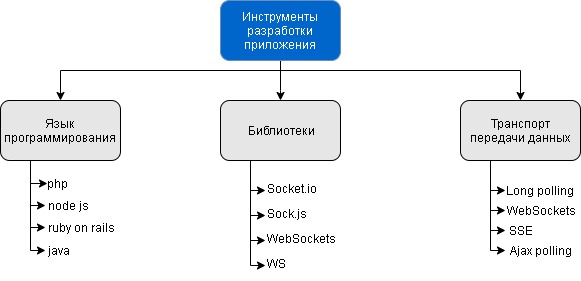
\includegraphics[scale=0.7]{my_folder/images/ApplicationDevelopmentTools}
	\caption{Инструменты разработки приложения}
	\label{fig:ApplicationDevelopmentTools}
\end{figure}
	
\subsection{Языки программирования} \label{ch2:subsec-abbr-programming-languages} %название по-русски









	
%%% ВНИМАНИЕ: для того, чтобы избежать лишнего отступа между текстом  и формулами, пожалуйста, начинайте формулы без пропуска строки в исходном коде как в строках #2 и #3.
Одиночные формулы также, как и отдельные формулы в составе группы, могут быть размещены в несколько строк. Чтобы выставить номер формулы напротив средней строки, используйте окружение \verb|multlined| из пакета \verb|mathtools| следующим образом \cite{Ganter1999}:
\begin{equation} % \tag{S} % tag - вписывает свой текст 
\label{eq:fConcept-order-G}
\begin{multlined}
(A_1,B_1)\leq (A_2,B_2)\; \Leftrightarrow \\  \Leftrightarrow\; A_1\subseteq A_2\; \Leftrightarrow \\ \Leftrightarrow\; B_2\subseteq B_1. 
\end{multlined}
\end{equation}

	
Используя команду \verb|\labelcref{...}| из пакета \verb|cleveref|, допустимо оформить ссылку на несколько формул, например, (\labelcref{eq:UpArrow-G,eq:DownArrow-G,eq:fConcept-order-G}). % пример оформления одиночной формулы в несколько строк

%Пример оформления четырёх иллюстраций в одном текстово-графическом объекте приведён на \firef{fig:spbpu_sc-four-photos}. Это возможно благодаря использованию пакета \verb|subcaption|.

\begin{figure}[ht]
	\adjustbox{minipage=1.3em,valign=t}{\subcaption{}\label{fig:spbpu_sc-a}}%
	\begin{subfigure}[t]{\dimexpr.5\linewidth-1.3em\relax}
		\centering
		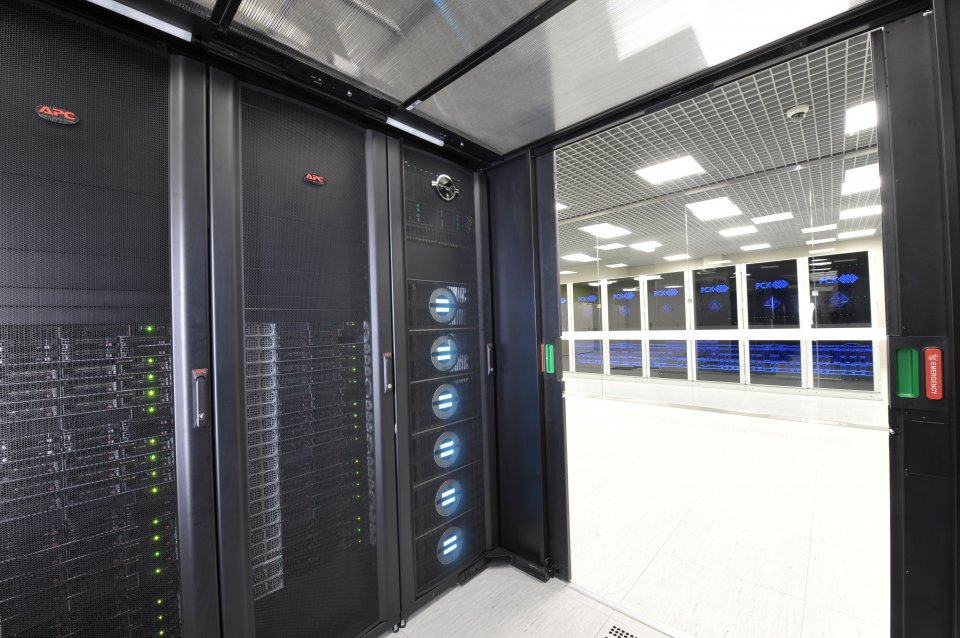
\includegraphics[width=.95\linewidth,valign=t]{my_folder/images/spbpu_sc_system}
	\end{subfigure}
\hfill %выровнять по ширине
	\adjustbox{minipage=1.3em,valign=t}{\subcaption{}\label{fig:spbpu_sc-b}}%
	\begin{subfigure}[t]{\dimexpr.5\linewidth-1.3em\relax}
		\centering
		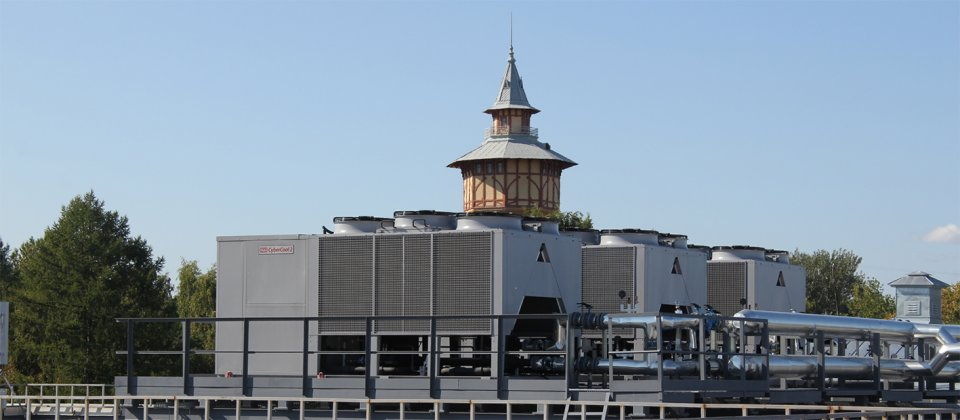
\includegraphics[width=.95\linewidth,valign=t]{my_folder/images/spbpu_sc_refr}
	\end{subfigure}
\\[20pt]
	\adjustbox{minipage=1.3em,valign=t}{\subcaption{}\label{fig:spbpu_sc-c}}%
\begin{subfigure}[t]{\dimexpr.5\linewidth-1.3em\relax}
	\centering
	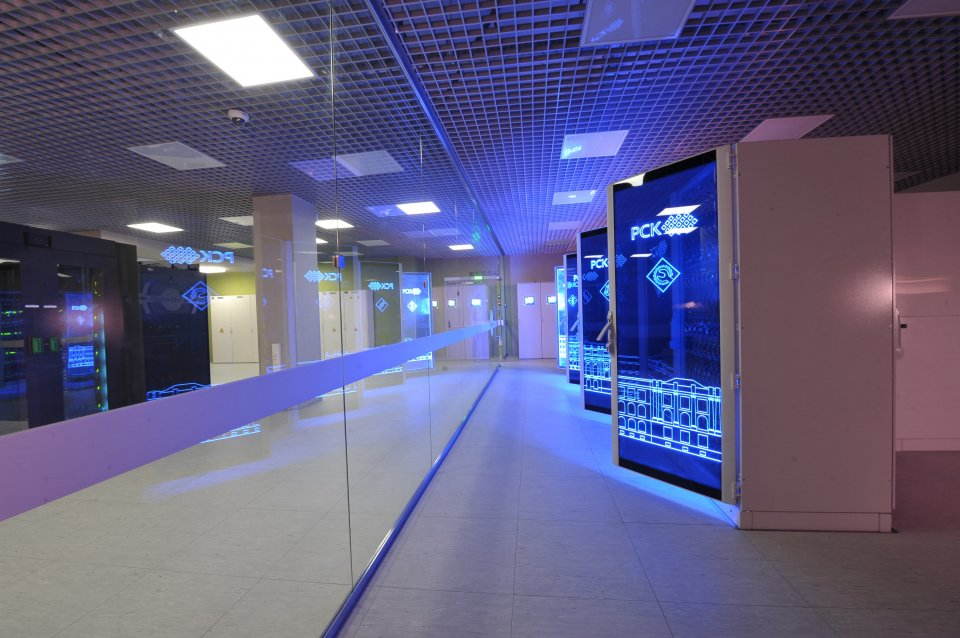
\includegraphics[width=.95\linewidth,valign=t]{my_folder/images/spbpu_sc_hall}
\end{subfigure}%
\hfill %выровнять по ширине
\adjustbox{minipage=1.3em,valign=t}{\subcaption{}\label{fig:spbpu_sc-d}}%
\begin{subfigure}[t]{\dimexpr.5\linewidth-1.3em\relax}
	\centering
	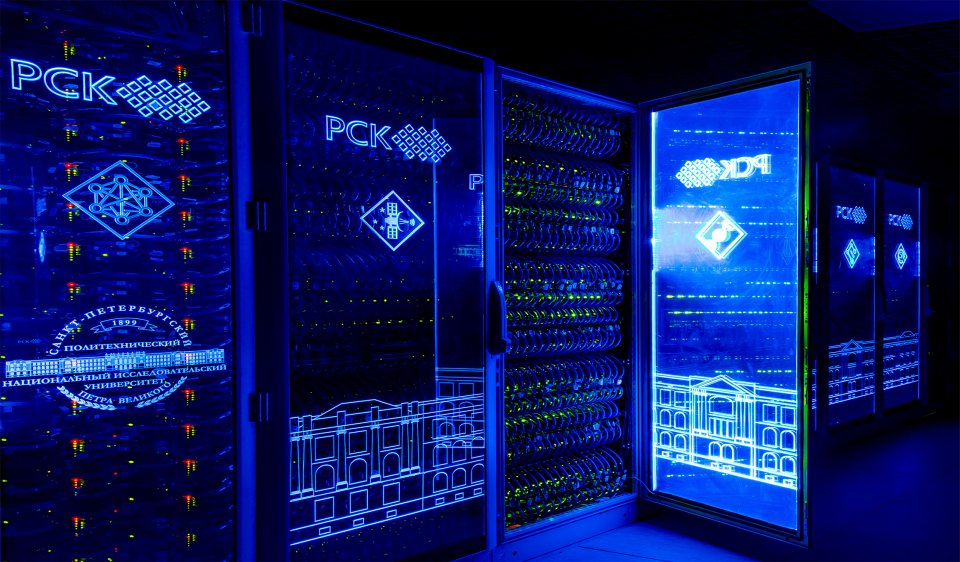
\includegraphics[width=.95\linewidth,valign=t]{my_folder/images/spbpu_sc_box}
\end{subfigure}
\captionsetup{justification=centering} %центрировать
\caption{Фотографии суперкомпьютерного центра СПбПУ \cite{spbpu-gallery}: {\itshape a} --- система хранения данных и узлы NUMA-вычислителя; {\itshape b} --- холодильные машины на крыше научно-исследовательского корпуса; {\itshape c} --- машинный зал; {\itshape d} --- элементы вычислительных устройств} 
\label{fig:spbpu_sc-four-photos}
\end{figure}

Далее можно ссылаться на составные части данного рисунка как на самостоятельные объекты: \firef{fig:spbpu_sc-a}, \firef{fig:spbpu_sc-b}, \firef{fig:spbpu_sc-c}, \firef{fig:spbpu_sc-d} или на три из четырёх изображений одновременно: рис.\labelcref{fig:spbpu_sc-a,fig:spbpu_sc-b,fig:spbpu_sc-c}. % пример подключения 4х иллюстраций в одном рисунке

%На \firef{fig:spbpu_whitehall-three-photos} приведены три картинки под~общим номером и~названием, но с раздельной нумерацией подрисунков посредством пакета \verb|subcaption|.
%
\begin{figure}[!htbp]
	\adjustbox{minipage=1.3em,valign=t}{\subcaption{}\label{fig:spbpu_whitehall-a}}%
	\begin{subfigure}[t]{\dimexpr.3\linewidth-1.3em\relax}
		\centering
		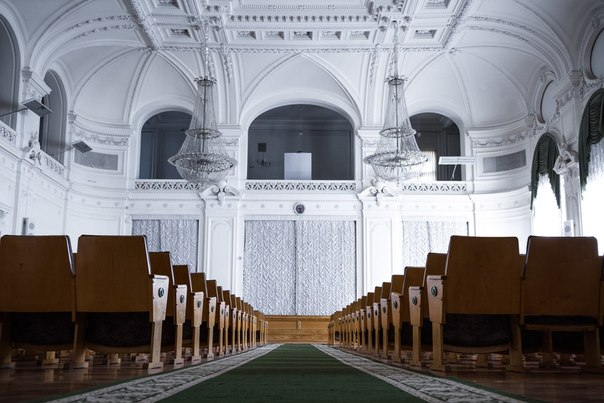
\includegraphics[width=.95\linewidth,valign=t]{my_folder/images//spbpu_whitehall}
	\end{subfigure}
	\hfill %выровнять
	\adjustbox{minipage=1.3em,valign=t}{\subcaption{}\label{fig:spbpu_whitehall-b}}%
	\begin{subfigure}[t]{\dimexpr.3\linewidth-1.3em\relax}
		\centering
		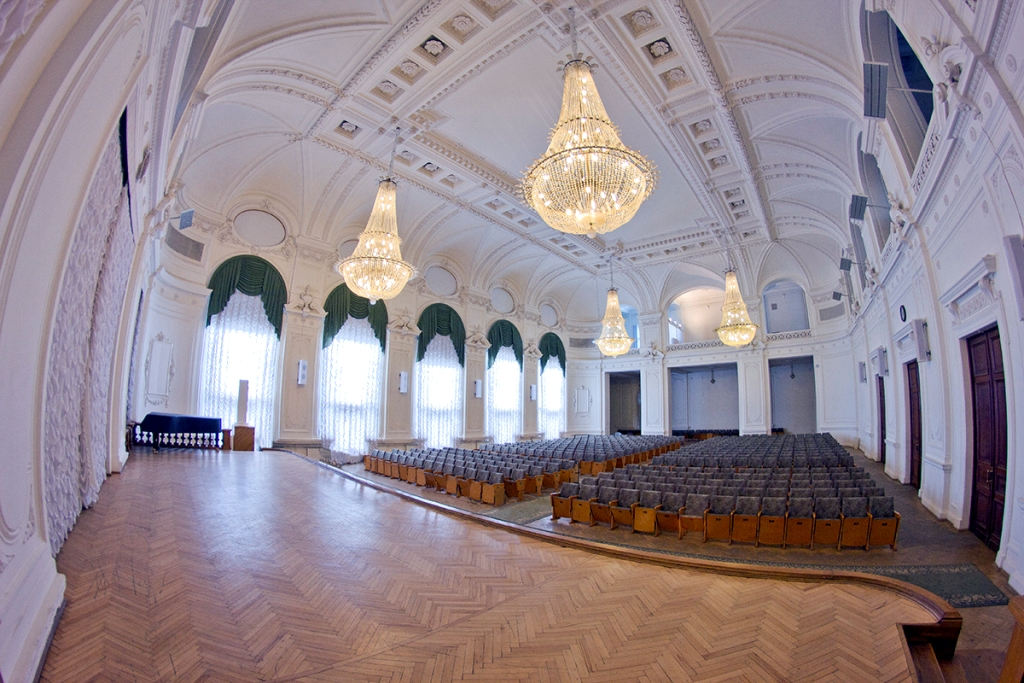
\includegraphics[width=.95\linewidth,valign=t]{my_folder/images//spbpu_whitehall_ligh}
	\end{subfigure}
	\hfill %выровнять
		\adjustbox{minipage=1.3em,valign=t}{\subcaption{}\label{fig:spbpu_whitehall-c}}%
	\begin{subfigure}[t]{\dimexpr.3\linewidth-1.3em\relax}
		\centering
		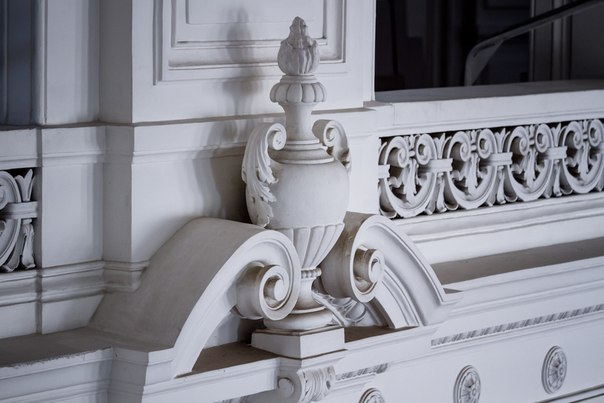
\includegraphics[width=.95\linewidth,valign=t]{my_folder/images//spbpu_whitehall_sculpture}
	\end{subfigure}%
\captionsetup{justification=centering} %центрировать
	\caption{Фотографии Белого зала СПбПУ \cite{spbpu-gallery}, в том числе: {\itshape a} --- со стороны зрителей; {\itshape b} --- со стороны сцены; {\itshape c} --- барельеф}\label{fig:spbpu_whitehall-three-photos}  
\end{figure}

Далее можно ссылаться на три отдельных рисунка: \firef{fig:spbpu_whitehall-a}, \firef{fig:spbpu_whitehall-b} и \firef{fig:spbpu_whitehall-c}. % пример подключения 3х иллюстрации в одном рисунке
%
%На \firef{fig:spbpu_main_bld-two-photos} приведены две картинки под~общим номером и~названием.


\begin{figure}[!htbp]
	\adjustbox{minipage=1.3em,valign=t}{\subcaption{}\label{fig:spbpu_main_bld_entrance_autumn}}%
	\begin{subfigure}[t]{\dimexpr.5\linewidth-1.3em\relax} %разрешили выделить 0,5 стр в ширину на рисунок
		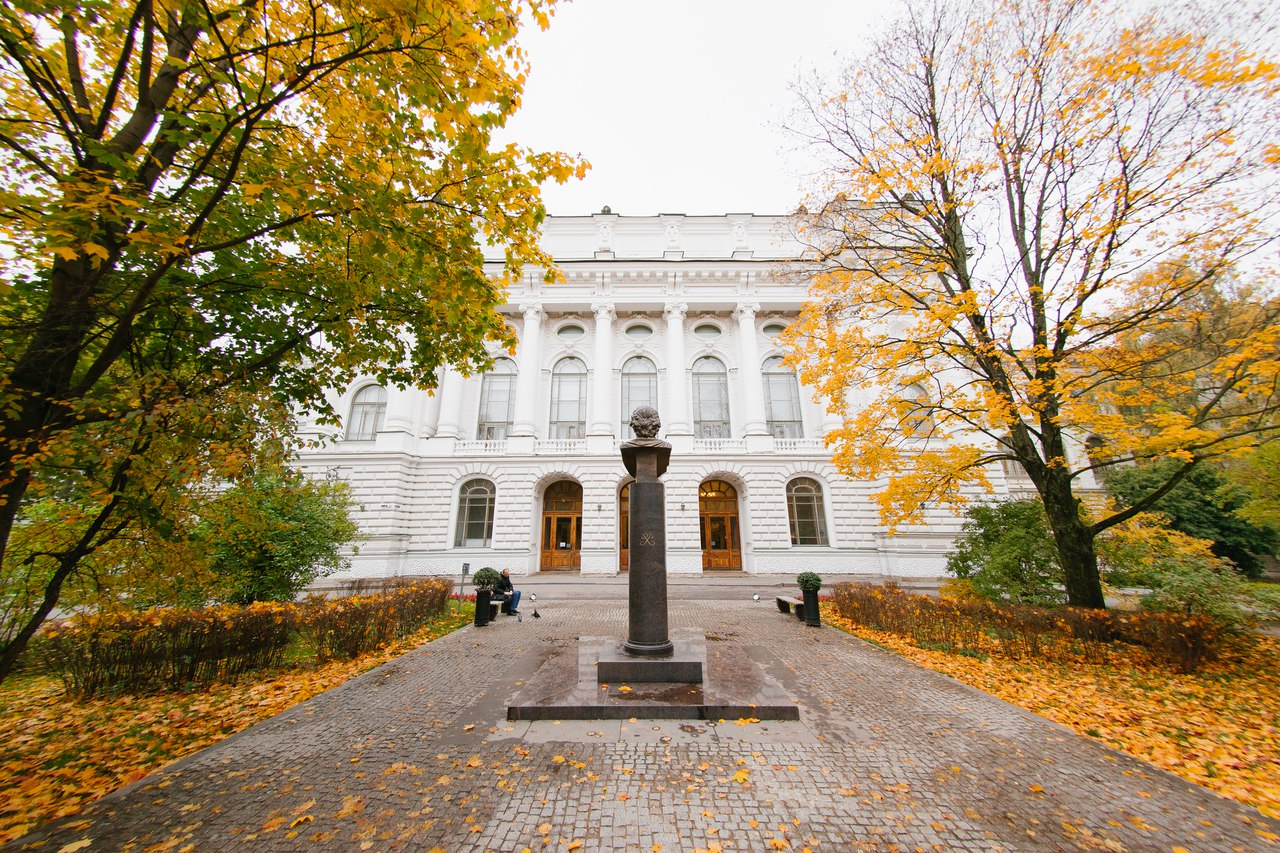
\includegraphics[height=0.20\textheight,valign=t]{my_folder/images//spbpu_main_bld_entrance_autumn} %высоту рисунка выставили как 0,3 от высоты наборного поля
	\end{subfigure}
%	\hfill %выровнять по ширине
	\adjustbox{minipage=1.3em,valign=t}{\subcaption{}\label{fig:spbpu_main_bld_whitehall}}%
	\begin{subfigure}[t]{\dimexpr.5\linewidth-1.3em\relax}%разрешили выделить 0,5 стр в ширину на рисунок
		
\includegraphics[height=0.20\textheight,valign=t]{my_folder/images//spbpu_main_bld_whitehall}%высоту рисунка выставили как 0,3 от высоты наборного поля
	\end{subfigure}
\captionsetup{justification=centering} %центрировать
	\caption{Вид на главное здание СПбПУ \cite{spbpu-gallery}, включая: {\itshape a} --- вход со стороны парка осенью; {\itshape b}~--- окна Белого зала}\label{fig:spbpu_main_bld-two-photos} 
\end{figure}

На \firef{fig:spbpu_main_bld_entrance_autumn} изображен вход со стороны парка СПбПУ осенью, а на \firef{fig:spbpu_main_bld_whitehall}~--- окна Белого зала. % пример подключения 2х иллюстраций в одном рисунке

%Приведём пример табличного представления данных с записью продолжения на следующей странице на \taref{tab:long}.

%%% отладка longtable
%% 1) для контроля выхода таблицы за границы полей выставляем showframe в \geometry{}, см настройки
%% 2) используем \\* для запрета переноса определенной строки или средства из:
%% https://tex.stackexchange.com/q/344270/44348
%% 3) в крайнем случае для принудительного переноса таблицы на новую страницу используем \pagebreak после \\
\noindent % for correct centering
\begingroup
\centering
\small %выставляем шрифт в 12bp
\begin{longtable}[c]{|l|l|l|l|l|l|}
	\caption{Пример задания данных из \cite{Peskov2004} (с повтором для переноса таблицы на новую страницу)}%
	\label{tab:long}% label всегда желательно идти после caption
	\\
	\hline
	$G$&$m_1$&$m_2$&$m_3$&$m_4$&$K$\\ \hline
	1&2&3&4&5&6\\ \hline
	\endfirsthead%
	\captionsetup{format=tablenocaption,labelformat=continued} % до caption!
	\caption[]{}\\ % печать слов о продолжении таблицы
	\hline
	1&2&3&4&5&6\\ \hline
	\endhead
	\hline
	\endfoot
	\hline
	\endlastfoot
	$g_1$&0&1&1&0&1\\ \hline
	$g_2$&1&2&0&1&1\\ \hline
	$g_3$&0&1&0&1&1\\ \hline
	$g_4$&1&2&1&0&2\\ \hline
	$g_5$&1&1&0&1&2\\ \hline
	$g_6$&1&1&1&2&2\\ \hline
%
	$g_1$&0&1&1&0&1\\ \hline 
	$g_2$&1&2&0&1&1\\ \hline
	$g_3$&0&1&0&1&1\\ \hline
	$g_4$&1&2&1&0&2\\ \hline \noalign{\penalty-5000} % способствуем переносу на следующую стр
	$g_5$&1&1&0&1&2\\ \hline 
	$g_6$&1&1&1&2&2\\ \hline
%
	$g_1$&0&1&1&0&1\\ \hline 
	$g_2$&1&2&0&1&1\\ \hline
	$g_3$&0&1&0&1&1\\ \hline
	$g_4$&1&2&1&0&2\\ \hline
	$g_5$&1&1&0&1&2\\ \hline
	$g_6$&1&1&1&2&2\\ \hline
%		
	$g_1$&0&1&1&0&1\\ \hline 
	$g_2$&1&2&0&1&1\\ \hline
	$g_3$&0&1&0&1&1\\ \hline
	$g_4$&1&2&1&0&2\\ \hline
	$g_5$&1&1&0&1&2\\ \hline
	$g_6$&1&1&1&2&2\\ \hline
%
	$g_1$&0&1&1&0&1\\ \hline 
	$g_2$&1&2&0&1&1\\ \hline
	$g_3$&0&1&0&1&1\\ \hline
	$g_4$&1&2&1&0&2\\ \hline
	$g_5$&1&1&0&1&2\\ \hline
	$g_6$&1&1&1&2&2\\ \hline
%
	$g_1$&0&1&1&0&1\\ \hline 
	$g_2$&1&2&0&1&1\\ \hline
	$g_3$&0&1&0&1&1\\ \hline
	$g_4$&1&2&1&0&2\\ \hline
	$g_5$&1&1&0&1&2\\ \hline
	$g_6$&1&1&1&2&2\\ \hline
%
	$g_1$&0&1&1&0&1\\ \hline 
	$g_2$&1&2&0&1&1\\ \hline
	$g_3$&0&1&0&1&1\\ \hline
	$g_4$&1&2&1&0&2\\ \hline
	$g_5$&1&1&0&1&2\\ \hline
	$g_6$&1&1&1&2&2\\ \hline
\end{longtable}
\normalsize% возвращаем шрифт к нормальному
\endgroup % пример подключения таблицы на несколько страциц








Выбор правильного языка программирования имеет решающее значение в разработке приложения. Проведём исследование языков программирования, подходящих для серверной веб-разработки, таких как Python, Node.js, Java, PHP. Языки сравниваются по общей популярности, поддержке облачных провайдеров, производительности и доступным интеграциям.

\textbf{Python} – это интерпретируемый объектно-ориентированный язык программирования высокого уровня с динамической семантикой. Его встроенные структуры данных высокого уровня в сочетании с динамической типизацией и динамическим связыванием делают его очень привлекательным для быстрой разработки приложений, а также для использования в качестве скриптового или связующего языка для соединения существующих компонентов. Python поддерживает модули и пакеты, что способствует модульности программы и повторному использованию кода. Интерпретатор Python и обширная стандартная библиотека доступны для всех основных платформ.

\textbf{Node.js} – это среда, которая позволяет использовать JavaScript как для backend, так и для frontend разработки, а также для решения проблем совместимости. Его также можно определить как язык сценариев на стороне сервера. Он хорош для обработки проектов с множеством одновременных подключений или приложений с высокоскоростным и интенсивным вводом / выводом (I/O), а также приложений, таких как платформы повышенной производительности (например, системы управления контентом), торговые площадки P2P и платформы электронной коммерции.

\textbf{Java} – это объектно-ориентированный и параллельный язык программирования общего назначения, разработанный Sun Microsystems в 1995 году. Он использует механизм под названием JVM (виртуальная машина Java), который обеспечивает среду выполнения для запуска кода Java и его приложений. Он переводит байт-код Java в язык, который может интерпретироваться машинами. JVM является частью JRE (Java Runtime Environment).

\textbf{PHP} – это язык программирования, созданный для создания веб-приложений, построенный на языке программирования C и использующий уникальные HTML-подобные теги для содержания своего кода. Язык программирования PHP в основном используется на стороне сервера, что означает, что он работает на программном обеспечении вашего веб-сервера, которое обычно будет обслуживать HTML ваших посетителей.


\begin{table}
	\caption{Сравнение языков программирования  \cite{PHPvsPyt48:online,NodejsVs38:online} Приложение \cite{appendix:comparationPL}}
	\label{comparisonOfProgrammingLanguage}
	\begin{tabularx}{\linewidth}{|X|X|X|X|X|}
		\hline
		& Python & Node Js & Java & PHP \\
		\hline
		Наличие библиотек & Обладает исключительно хорошо развитой библиотечной поддержкой практически для всех типов приложений & Обладает исключительно хорошо развитой библиотечной поддержкой практически для всех типов приложений & Hibernate, Swing, SWT (Standard Widget Toolkit) & Packagist (репозиторий пакетов PHP) является сильной основой, поддерживающей PHP \\
		\hline
		Доступ к базам данных & Не сильная интеграция базы данных & Он обеспечивает доступ к более чем 20 различным базам данных & Он обеспечивает доступ к более чем 20 различным базам данных & Он обеспечивает доступ к более чем 20 различным базам данных \\
		\hline
		Скорость работы & 4/5 & 5/5 & 5/5 & 4/5 \\
		\hline
		Наличие фреймворков & Django, Flask, Pylons, Pyramid & Express.js, Meteor.js, Koa.js & Java Server Faces (JSF), Stuts2, Spring & Codeigniter, Zend, Laravel, Symfony \\
		\hline
	\end{tabularx}
\end{table}

Наилучшим языком программирования, согласно представленным критериям и по расчётам  метода Саати – является Java (Приложение \ref{appendix:methodSaati}). Из этого следует, что такой подход предоставляет лучшее решение из представленных вариантов, однако в разработке для сервера будет использоваться Node js (согласно требованиям заказчика).

\subsection{Библиотеки}

Чтобы обеспечить двустороннюю связь клиента с сервером выделим решения, считающиеся популярными, для работы с web sockets и Node.js.

Socket.io – это библиотека позволяет установить двунаправленную связь между клиентом и сервером. Для корректной работы библиотеки, ей необходимо установить как на клиентской стороне, так и на серверной Node js. API у компонент (клиентская, серверная) – идентичен и управляет событиями. Socket.IO напоминает WebSockets. WebSockets также является браузерной реализацией, позволяющей осуществлять двунаправленную связь, однако Socket.IO не использует это в качестве стандарта. Во-первых, Socket.IO создает соединение с длинным опросом, используя xhr-опрос. Затем, как только это установлено, он обновляется до наилучшего способа подключения. В большинстве случаев это приведет к соединению WebSocket. Хотя Socket.IO может использоваться в качестве оболочки для WebSocket так как предоставляет больший функционал, включая широковещательную передачу на несколько сокетов, асинхронный ввод-вывод и хранение данных.

Sock.js - то JavaScript-библиотека браузера, которая предоставляет объект, подобный WebSocket. SockJS предоставляет вам согласованный кросс-браузерный API Javascript, который создает полнодуплексный междоменный канал связи с низкой задержкой между браузером и веб-сервером.

Произведём сравнение WebSocket \cite{WebSocke16:online} с популярными библиотеками \cite{Introduc57:online,SockJS·G77:online}, работающими на этом протоколе, однако предлагающими больший функционал. Для сравнения были разработаны клиенты и серверы (Приложения \ref{appendix:serverSideBySocketIO}, \ref{appendix:serverSideBySockJS}), используя express.js (фреймворк для создания сервера Node.JS).



\begin{figure}
	\centering
	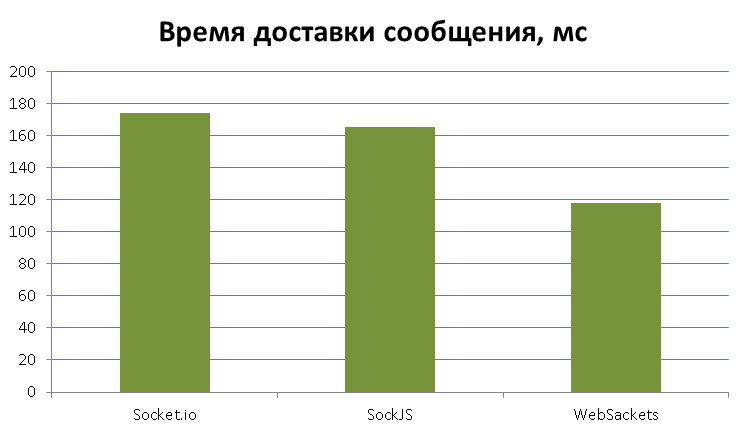
\includegraphics[scale=0.7]{my_folder/images/speedMessageDeliver}
	\caption{Сравнение времени опроса}
	\label{fig:speedMessageDeliver}
\end{figure}

\subsection{Мониторинг}
\label{Moninoring}

%\FloatBarrier % заставить рисунки и другие подвижные (float) элементы остановиться
Так как веб-серверы обрабатывают запросы пользователей на контент, то это непосредственно отражается на производительности и заметное влияние на взаимодействие с пользователя. Если веб-серверы работают медленно, пользователи откажутся от его услуг. Поэтому Application Performance Monitoring (APM) необходим для проекта. Он предупредит вас о любых ошибках или сбоях, которые могут привести к простою и о возможных сбоях.

Одним из основных преимуществ мониторинга – автоматизация. Сайты высокой ежедневной проходимостью часто оптимизируют пропускную способность балансировкой нагрузки, когда запросы делегируются на несколько веб-серверов. Отдельная служба балансировки нагрузки принимает входящие запросы, проверяет доступность веб-серверов, расположенных за ней, и передает запрос на доступный сервер. Для этого балансировщик нагрузки должен знать текущую нагрузку каждого веб-сервера и его доступность для обработки новых запросов.

Наконец, мониторинг помогает отслеживать популярность и рост веб-сайтов и веб-приложений. Метрики трафика и подключений позволяют получить непосредственное представление об активности сайта, в том числе о количестве активных пользователей и продолжительности каждого сеанса. Эти данные могут помочь вам разработать планы по масштабированию вашего веб-сайта, оптимизации вашего приложения или развертыванию других служб для поддержки возросшего спроса.

\textbf{New Relic} – является одним из самых популярных инструментов в среде APM. Он предоставляет информацию о многих типах программных и аппаратных компонентов или о взаимодействии с пользователем и поддерживает множество технологий, либо через своих собственных агентов, либо через внешние плагины. Одной из лучших функций является подробный мониторинг транзакций, обеспечивающий отслеживание между приложениями и отслеживание производительности операторов SQL. \cite{NewRelic78:online}

Преимущества:
\begin{itemize}
	\item Дружественный пользовательский интерфейс;
	\item Очень хорошо в нахождении корреляции данных;
	\item Включает отслеживание транзакций и процессов;
	\item Хороший форум сообщества и поддержка.
\end{itemize}

Недостатки:
\begin{itemize}
	\item Предоставляется только по SaaS (нет локальной версии);
	\item Хранение данных зависит от уровня подписки, но в лучшем случае сохраняет все данные в течение 8 дней (после сохраняет только усреднённые данные);
	\item Ценообразование. Стоимость подписки начинается примерно с 60 долларов США за месяц и увеличивается в зависимости от многих аспектов (уровня подписки, компонентов мониторинга, количества серверов и т. д.). С другой стороны, он имеет бесплатную версию Lite, но она сильно урезана и имеет только 2 часа хранения ограниченного количества данных (строго определённых).
\end{itemize}

\textbf{CloudWatch} – это инструмент мониторинга и управления Amazon Web Service (AWS). Он предоставляет данные о производительности компонентов AWS и приложений, работающих в инфраструктуре Amazon. CloudWatch имеет базовый мониторинг, который является бесплатным для пользователей AWS, а так же подобрав тарифный план его можно улучшить. Предоставляя такие функции, как более подробный мониторинг, пользовательские метрики и многое другое. Однако пользовательский интерфейс может быть немного сложным для людей, не имеющих опыта работы с подобными инструментами.\cite{AmazonCl81:online}

Преимущества:
\begin{itemize}
	\item Бесплатная версия (для пользователей AWS) предлагает достаточно ресурсов для базового мониторинга приложения;
	\item Настраиваемые панели для отображения метрик и графиков;
	\item Гибкие низкие цены.
\end{itemize}

Недостатки:
\begin{itemize}
	\item Он может использоваться только для компонентов AWS и, следовательно, для приложений, работающих только на серверах Amazon. Есть несколько скриптов, созданных сторонними разработчиками, для получения метрик для серверов не-AWS, но они не являются «официальным»;
	\item Пользовательский интерфейс не очень удобен для анализа данных, что затрудняет выполнение корреляции данных;
	\item Нет отслеживания транзакций;
	\item По умолчанию нет метрик использования памяти. Пользовательский показатель должен быть настроен для мониторинга этого основного индикатора.
\end{itemize}

\textbf{Dynatrace APM} – предлагает мониторинг производительности и управление приложениями как в модели SaaS, так и на локальном сервере. Он поддерживает несколько технологий, имеет глубокую трассировку транзакций, мониторинг взаимодействия с пользователем (синтетический мониторинг и мониторинг реального пользователя) и мониторинг сети. Так присутствует функция, которая автоматически обнаруживает все компоненты сервера и быстро запускает отчетные данные на разных уровнях после его установки. Даже время загрузки страницы сообщается путем внедрения JavaScript в ваше веб-приложение.\cite{Applicat35:online}

Преимущества:
\begin{itemize}
	\item Простота установки и настройки;
	\item Бесплатная версия позволяет контролировать до 5 серверов в течение неограниченного времени, без ограничений функциональности или срока хранения данных. Там количество посещений ограничено 100к;
	\item Обнаруживает топологию приложений, развертывания и изменения среды в режиме реального времени;
	\item Отлично подходит для отслеживания транзакций и процессов.
\end{itemize}

Недостатки: 
\begin{itemize}
	\item Пользовательский интерфейс немного сложен, особенно для пользователей, не имеющих опыта работы с подобными инструментами;
	\item Ценообразование. Несмотря на то, что бесплатная версия действительно хороша для небольших инфраструктур (5 серверов или меньше), платные опции имеют цены, аналогичные New Relic.
\end{itemize}


\textbf{AppDynamics} – несколько лет назад этот инструмент был основным современным программным обеспечением для мониторинга APM. Рассматривая некоторые функции AppDynamics (например, главный экран с картой служб, используемых с их нагрузкой на вызов и индексом работоспособности, или мониторами взаимодействия с пользователем), создается впечатление, что приоритетами мониторинга инструментов являются крупные предприятия с большой инфраструктурой.\cite{Theworld87:online}

Преимущества:
\begin{itemize}
	\item Дружественный пользовательский интерфейс с настраиваемыми инструментальными панелями;
	\item Хороший мониторинг ресурсов сервера;
	\item Включает транзакции и отслеживание процессов;
	\item Использует алгоритмы машинного обучения, чтобы установить базовые значения для установки оповещения.
\end{itemize}

Недостатки:
\begin{itemize}
	\item Некоторые функции инструмента основаны на Flash, и вы не можете использовать их, не включив его в браузере;
	\item Ценообразование. AppDynamics нет цен, опубликованных на веб-странице, вам придется связаться с отделом продаж, чтобы получить индивидуальный план и стоимость, основанные на ваших потребностях.
\end{itemize}


\textbf{CA Technologies APM} – одной из основных характеристик инструмента CA APM является то, что это гибкое и настраиваемое программное обеспечение: компания предлагает службу поддержки, которая позволяет настраивать особый мониторинг и оповещения для получения более точных и полезных данных для каждого специфическая для компании ситуация. 

CA APM имеет настраиваемые панели мониторинга, многоперспективные представления о работе конечных пользователей, автоматические трассировки транзакций и множество показателей ресурсов инфраструктуры.\cite{Applicat77:online}

Преимущества:
\begin{itemize}
	\item Универсальный инструмент, так как компания CA готова адаптировать инструмент для нужд клиента;
	\item Team Center предоставляет настраиваемую панель инструментов для быстрой навигации по деталям, чтобы разобраться в проблемах;
	\item Включает отслеживание транзакций и процессов;
	\item Хорошая поддержка и форум сообщества.
\end{itemize}

Недостатки:
\begin{itemize}
	\item Это может потребовать довольно большой кривой обучения, особенно для людей, не имеющих опыта работы с такими инструментами;
	\item Цены могут быть немного высокими для небольших инфраструктур.
\end{itemize}



\begin{table}
	\caption{Сравнение APM}
	\label{comparisonOfAPM}
	\begin{tabularx}{\linewidth}{|p{1.8cm}|X|X|X|X|X|}
		\hline
	& User Interface &	SaaS/ Local server	& Transaction trecking	& Data correlation & Support services\\
		\hline
		New Relic &	Простой и понятный интерфейс &	SaaS	& Подробный мониторинг транзакций	& Хорошо реализован	& Имеется \\
		\hline
		Cloud Watch &	Требует определённые навыки работы в данной сфере & 	SaaS и локальный сервер (только для AWS) & 	Отсутствует	& Имеется, слабая реализация	& Имеется, но только для клиентов AWS \\
		\hline
		Dynatrace APM	& В начале кажется сложным, но к нему быстро привыкнуть	& SaaS и локальный сервер & 
		Отличное (подробное) отслеживание проходящих транзакций и процессов	& Хорошо реализован	& Имеется, но уровень помощи зависит от подписки \\
		\hline
		App Dynamics	& Простой и понятный интерфейс, только используется Flash	& SaaS и локальный сервер	& Подробный мониторинг транзакций	& Имеется	& Имеется \\
		\hline
		CA APM	& Простой и понятный интерфейс	& SaaS и локальный сервер	& Подробный мониторинг транзакций	& Хорошо реализован	& Имеется \\
		\hline		
	\end{tabularx}
\end{table}

\newpage

%%%%%%%%%%%%%%%%%%%%%%%%%%%%%%%%%%%%%%%%%%%%
%
%    Не забыть поменять ссылку на Приложение 
%
%%%%%%%%%%%%%%%%%%%%%%%%%%%%%%%%%%%%%%%%%%%%
Наилучшей системой мониторинга, согласно представленным критериям и по расчётам  метода Саати – является Dynatrace APM (Приложение \ref{appendix:choosingMonitoringSys}). Из этого следует, что такой подход предоставляет лучшее решение мониторинга из выше представленных.


\subsection{Веб-хостинг}
\label{web_hosts}

\subsubsection{Виды хостингов}
\label{typeOfHosts}

Выбирать хостинг, на котором будет размещаться высокопроизводительное веб-приложение – это ещё один важный пункт. Если все сделано правильно, вы можете провести целую жизнь счастья с надежным и высокопроизводительным хостом, который всегда доступен по телефону, чату или электронной почте, чтобы ответить на ваши горящие ночные вопросы. Однако спешка в отношении выбора хостинга, без проведения исследования, может привести к тому, что вы окажетесь в ловушке, введены в заблуждение или даже стать жертвой вымогательства со стороны хостинга. Выбор неправильного хоста часто заканчивается головными болями и дорогим разводом.

Чтобы не переплачивать и быть обманутым надо чётко понимать, какой вид хостинга вам необходим. Если рассматривать, то все хостинги можно разделить на следующие виды.

\textbf{Общий хостинг (виртуальный)}. В нём несколько клиентов и веб-сайтов используют один и тот же сервер. С одной стороны, виртуальный хостинг - это классический вид, с которого начинают развитие все малые и средние веб-приложения - простой и несложный. Не всегда, запуская веб-приложение малого или среднего бизнеса, можно выйти за рамки предоставляемые хостингом по памяти и ресурсам процессора. Лишь когда приложение набирает обороты необходимо решать, когда пора перейти на VPS или выделенный план для удовлетворения ваших растущих потребностей. Однако с другой точки зрения виртуальный хост ограничивает вас с сотнями или тысячами других. Поскольку ресурсы сервера распределены между очень многими сайтами, производительность иногда снижается по мере роста вашего сайта. Если вы готовы серьезно и реально увеличить свой трафик, вы, вероятно, не захотите соглашаться с общим планом хостинга. 

Цена, поддержка, хранение и производительность - все это важные характеристики, которые следует учитывать при покупке общего хостинга. Другие отличия включают предложения электронной коммерции и бесплатные варианты доменов, а также такие привилегии, как рекламные кредиты, конструктор сайтов и модернизированное оборудование.

\textbf{VPS хостинг}. Virtual private server (VPS) – является промежуточным звеном между общим хостингом и выделенным сервером. Сервер разделен на виртуальные машины, которые действуют как независимые выделенные серверы. Клиенты VPS по-прежнему имеют общий сервер, но у каждого из них гораздо большие ресурсов и больший контроль, чем у тех, у кого есть план общего хостинга. 

Поскольку вы можете добавлять или удалять дополнительные вычислительные ресурсы по мере необходимости, планы хостинга VPS могут расширяться. У вас может быть довольно крупный основной сервер, но это не значит, что вы не можете подключить еще дополнительные мощностей в режиме ожидания.

Хосты VPS обычно включают в себя хранилище с высокоскоростными твердотельными накопителями или твердотельными накопителями, а также управляемые службы для обновления программного обеспечения. В зависимости от вашего уровня технического мастерства, вы можете пользоваться бесплатной панелью управления или, используя полный доступ прав root, настроить инфраструктуру самому. Вы также увидите, что топ-хосты VPS включают службы мониторинга, безопасности и CDN, чтобы держать вас осведомлённым.

\textbf{Выделенный хостинг}.  Для высокопроизводительных сайтов требуется выделенный хостинг, что подразумевает использование всего сервера для питания вашего сайта или приложений. Как видно из названия, выделенные серверы готовы подождать с вами и идти навстречу и удовлетворить все ваши потребности в конфигурации. Клиенты имеют полный контроль над архитектурой, то есть они могут настраивать системы безопасности, операционные системы, балансировщики нагрузки и многое другое. 

Однако это не обходится дешево. Выделенные планы хостинга являются одними из самых дорогих, учитывая первоклассное оборудование, управляемые услуги и круглосуточную поддержку. Однако хостинг высокого класса поставляется с рядом роскошных функций, включая автоматическую миграцию и резервное копирование, выделенные IP-адреса и выбор операционной системы.

\subsubsection{Виды веб-приложений}
\label{typesOfWebApp}

Следующим этапом для выбора хостинга, надо знать какой тип веб-приложения вы планируете реализовать. Количество ожидаемого трафика или нагрузки на сервер влияет на тип хостинг-плана, который вы хотите найти, а так же ваш тип сайта будет определять, какие функции наиболее важны. Например, некоторые хостинг-провайдеры продвигают функции электронной коммерции, в то время как другие концентрируются на блогах и поисковой оптимизации. Условно виды сайтов можно разделить на следующие группы.

\textbf{Блоги}. В связи с тем, что сайты на основе системы управления контента занимают более четверти рынка \cite{UsageSta21:online,NeedtoKn7:online} среди всех веб-сайтов в Интернете, сайты блого-подобного характера стали простым выбором для авторов, желающих поделиться своими мыслями в Интернете. Сейчас каждый хост предлагает оптимизированные установки под них, но лучшие провайдеры включают в себя обновленное оборудование, неограниченное хранилище и пропускную способность, предустановленные программы, а также специальные знания и круглосуточную поддержку.

\textbf{Интернет-магазины}. В 2016 году аналитическая компания comScore обнаружила, что потребители покупают в Интернете больше вещей, чем в магазинах\cite{2016UPSP16:online}. Более половины населения США совершают покупки в Интернете, поэтому компаниям следует найти веб-хостинга с широкими возможностями электронной коммерции. Ведущие хосты заботятся о дополнительных требованиях безопасности, связанных с защитой информации о клиентах и платежах, а также предоставляют красиво оформленные шаблоны, доступ к программному обеспечению корзины покупок и интеграцию с такими сервисами, как PayPal и инструменты почтового маркетинга.

\textbf{Сайты портфолио (персональные сайты)}. Соискателям становится важно иметь сайт визитку в Интернете, даже если желаемая отрасль не имеет ничего общего с веб-дизайном или маркетингом. Связанно это с тем, что это самый быстрый способ создать профессиональное присутствие в Интернете, которое демонстрирует вашу работу (ваш бизнес). Отличаются такие сайты тем, что это отличный способ создания небольших сайтов с ограниченным бюджетом, в который можно относительно легко перевести в отрасль электронной коммерции.

\textbf{Бизнес-сайты}.  Даже если вы не планируете использовать свой веб-сайт для продажи продуктов, ваш всё ещё бизнес рассчитывает на узнаваемость в Интернете как бренд. Предприниматели склонны ожидать, что их бизнес-сайт будет расти на 10-20\% каждый месяц, если все идёт согласно их плану, грамотно выбранный хостинг-провайдер сможет справиться с быстро развивающимся бизнесом.

\subsubsection{Виды ключевых ресурсов для веб-приложения}
\label{typeGeneralResorseOfWebApp} 

Определившись с типом веб-приложения, приходит понимание его особенностей и необходимых ресурсов. И тогда, выбирая хостинг, стоит ссылаться на соответствующие потребности веб-приложения, а не количестве предоставляемых услуг за меньшую плату. Например, компании могут отдавать предпочтение функциональности электронной почты над хранилищем, тогда как разработчик может предпочесть высокую пропускную способность и строгую безопасность. Если выделять технические особенности (ресурсы), то можно разбить их на следующие группы:

\textbf{Доменные имена}. Несмотря на то, что они обычно объединяются, регистрация доменов и веб-хостинг - это две разные услуги. Ваше доменное имя служит адресом вашего сайта и может быть зарегистрировано и размещено в компании, отличной от той, в которой размещены файлы вашего сайта. Держать все хостинговые ресурсы в одной хостинговой компании имеет в себе как и положительные так и негативные стороны. Из положительных можно выделить бесплатные переносы и миграции. Из негативных уменьшение уровня безопасности (но это правило работает не для всех хостингов).

\textbf{Адреса электронной почты}. Хостинг электронной почты особенно интересен владельцам бизнеса, которые хотят получить известность и признание имени, включив доменное имя в адреса электронной почты. Хостинг-провайдеры часто включают расширенные функции электронной почты, такие как службы пересылки и фильтрации, автоответчики и повышенную безопасность, для клиентов, которым требуется несколько почтовых ящиков или маркетинговых инструментов.

\textbf{Память и оперативная память}. Хранилище или дисковое пространство - это, пожалуй, самая простая для понимания функция хостинга, а также компонент, о котором вам, возможно, придется меньше всего беспокоиться. Многие провайдеры виртуального хостинга предлагают неограниченное хранилище; хотя это технически невозможно, большинство владельцев сайтов для частных лиц или предприятий малого бизнеса не приблизятся к достижению пределов. А когда вы переходите на VPS и выделенные планы, хранилище можно настраивать по мере необходимости.

Самая главное, на что нужно обращать внимание, когда дело доходит до хранилища веб-хостинга, это тип накопителя. Твердотельные накопители намного быстрее и надежнее, но стоят дороже. Традиционные жесткие диски, с другой стороны, чаще встречаются, поскольку обычно они имеют более высокую емкость и привлекательны для хостингов.

Как и в случае с персональным компьютером, ОЗУ в веб-хостинге служит аналогичной цели: быстрая обработка хранимых данных. Аппаратное обеспечение взаимодействует с дисками хранения для ускорения загрузки страниц, и многие считают ОЗУ одной из самых важных функций, которые следует учитывать при выборе хоста.

\textbf{Тарифы и надёжность}. Каждая секунда недоступности сайта\cite{HowMuchD49:online} может означать сотни упущенных возможностей продаж, подорвать репутацию бренда и потерю производительности. Отключение Amazon Web Services в начале 2017 года обошлось компаниям примерно в 150 миллионов долларов\cite{AmazonAn66:online} за три-четыре часа прерванного обслуживания.

Некоторые хосты гарантируют определенное количество времени безотказной работы и возмещают вам любые незапланированные отключения, помимо соглашения об уровне обслуживания. Гарантии, как правило, варьируются от 100\% до 99,9\%. Хоть большинство клиентов виртуального хостинга будут удовлетворены порогом безотказной работы 99,9\%, однако крупные компании предпочтут дополнительно заплатить за оставшиеся 0,1\%.

\textbf{Безопасность и поддержка}. Безопасность веб-сайта в значительной степени зависит от производимой работы администратора, однако  сама инфраструктура хостинговой компании может представлять одну из самых больших слабостей. Огромное количество веб-сайтов скомпрометированы из-за уязвимости хоста, поэтому обязательно, при поиске поставщиков услуг, стоит отдавать предпочтение тем, которые включают брандмауэры, службы мониторинга и другие надстройки безопасности. Большим плюсом будет ещё и автоматическое резервное копирование, если оно предоставляемо. 

Клиентам хостинга будет сложно найти провайдера, который не предлагает круглосуточную поддержку, но реальное исполнение возникших проблем – сильно разнится. Независимо от того, простой ли вопрос или требуется техническая помощь, служба поддержки всегда должна быть готова помочь. К сожалению, этот критически важный аспект хостинга трудно разглядеть, пока вы не начнёте работать с ними и не обнаружите, что вам нужна помощь. 


\section{Выводы} 
\label{ch2:conclusion}

Обладая чётким представлением какой тип веб-приложения разрабатываете и определив его ключевые ресурсы, можно уверено определить необходимый вид хостинга. С чётким представлением необходимого хостинга, остается только рассматривать просмотреть разные хостинг площадки на предмет необходимого плана или составления индивидуального плана. 

Кроме всего выше перечисленного присутствует ещё один вариант размещения своего веб-приложения. Покупка собственного сервера. Такой вариант имеет как и очевидные плюсы, так и недостатки. Плюсы:

\begin{itemize}[•]
	\item 	Полный контроль. Создавая собственный сервер, вы контролируете все его аспекты: архитектуру (процессор, оперативная память, хранилище и его тип и так далее), ОС, библиотеки и так далее.
	\item Стоимость. Если ваше веб-приложение имеет долгосрочный характер, то цена на эксплуатацию складывается из стоимости компонентов и потребляемой электроэнергии. Кроме этого, на вашем сервере может существовать не одно приложение, что опять же сокращает расходы в перспективе (данное уточнение справедливо для веб-приложений малого и среднего бизнеса).
\end{itemize}

Недостатки:

\begin{itemize}[•]
	\item Полный контроль. Обладая полным контролем над всеми аспектами веб сервера и веб-приложения, не гарантирует наличие достаточной квалификации для грамотной настройки всей инфраструктурой в целом. Кроме того собственный сервер, для стабильной работы веб-приложения, обязует вас постоянно проверять как аппаратное, так и программное состояние на предмет уязвимостей. В свою очередь хостинг берёт на себя обязательства в проверке и поддержании аппаратной и частично программной части.
	\item Трафик. Для собственного сервера необходимо создавать дополнительный договор с провайдером. Обычного клиентского договора спокойно хватает на 20-50 одновременных пользователей, что достаточно для личного пользования. Однако для бизнеса необходимо b2b планы, так как размещение по существующему договору сайт будет слишком медленный для доступа.
	\item Безопасность. Собственный сервер может не иметь такой же уровень надёжности, как предлагаемый хостингами. При сбоях питания и широкополосного подключения ваш веб-сайт также будет отключен до тех пор, пока не будет устранена неисправность. Так же самому необходимо обустраивать систему контроля резервных копий, которая предоставляется бесплатно в некоторых хостингах.
\end{itemize}

Размещение сайта на домашнем сервере может быть сделано, если вы знаете, что на самом деле делаете, а так же взвешены стоимость и выгода от этого. Если придётся тратить значительное время на изучение и покупку нового оборудования, обслуживание серверов и оплату увеличенных счетов за электроэнергию, возможно, нужно отказаться от этого, так как все ли эти проблемы. 

Надо понимать, что недорогая служба веб-хостинга имеет все функции, которые могут быстрее доставлять веб-контент своим клиентам. Это избавляет от необходимости самостоятельно управлять прерываниями питания и решать другие проблемы.


%% Вспомогательные команды - Additional commands
%
%\newpage % принудительное начало с новой страницы, использовать только в конце раздела
%\clearpage % осуществляется пакетом <<placeins>> в пределах секций
%\newpage\leavevmode\thispagestyle{empty}\newpage % 100 % начало новой страницы	         	 % Глава 2
\chapter{РАЗРАБОТКА МЕТОДИКИ ПО СОЗДАНИЮ ВЫСОКОНАГРУЖЕННЫХ ВЕБ-ПРИЛОЖЕНИЯХ} \label{ch3}

 
	
\section{Определение требований} \label{ch3:sec1}

В данной работе одной задачей является исследование основных источников угроз высоконагруженных веб-приложения. Основные угрозы для веб-приложений были рассмотрены и выявлены в первой главе настоящей работы. Так же обозначены специфичные угрозы для них.

Направлений разработки высоконагруженных веб-приложений – множество, каждое из них обладает своими потенциальными угрозами. Связанно это с тем, что высокие нагрузки – понятие относительное, как говорилось в первой главе. Однако все системы с высокой нагрузкой объединяет требовательность в ресурсах, как вычислительных, так и хранилищ. На основе этого сформируем методику разработки высоконагруженных систем, которая обобщит разные направления разработки, однако акцентирует внимание на обеспечении наименьшего показателя реакции системы.



\section{Разработка рекомендаций} \label{ch3:sec2}

Основные угрозы, нарушающие корректную работоспособность веб-приложения, были описаны в первой главе текущей работы. Так же были определены основные виды данных приложений. Основываться на это и на результаты работы \cite{AmazonAn66:online}, а так же на проведённый анализ в рамках исследования, в целях минимизации уязвимостей рекомендуется:

\begin{itemize}[•]
	\item Продумать архитектуру, согласно которой будет реализовываться высоконагруженное веб-приложение;
	\item Создание маршрутной карты;
	\item Определится с механизмами аутентификации и авторизации;
	\item Проводить фильтрацию всей вводимой информации;
	\item Хранить данные в зашифрованном виде;
	\item Определить и использовать специализированные http заголовки;
	\item Ограничить SQL запросы;
	\item Реализовать взаимоисключающий доступ к ресурсам или директориям;
	\item Производить http опрос, для подтверждения наличия соединения.
\end{itemize}

%\FloatBarrier % заставить рисунки и другие подвижные (float) элементы остановиться

\section{Обоснование выбора инструментария} \label{ch3:sec3}

Для разработки прототипа приложения был определён следующий стек технологий.

Разработка серверной части:

\textbf{Node js}. В качестве серверного языка была выбрана платформа Node js. Основной причиной данного выбора является требованием со стороны заказчика. Однако для внесения ясности скажу, что node js основан на движке V8 от компании Google. Особенностью этого движка заключается в том, что он экономно расходует память, неплохо оптимизирован, дает функционал по профилированию процессора и памяти. Так же комьюнити по всему миру трудятся над ним, что в свою очередь стремительно улучает его.

\textbf{Express.js} – фреймворк, созданный для упрощения разработки для веб-приложений и API. Был выбран в качестве дополнения при разработке сервера. Express уже является стандартным каркасом для разработчиков веб-приложений, так как упрощает базовые функции предоставляемые из коробки Node js.

\textbf{PostgreSQL} была выбрана в качестве СУБД. Связанно это с тем, что она предоставляется по бесплатной лицензии в плоть до коммерческого использования, поддерживает сложные запросы (выходящие за рамки базовых SQL запросов), позволяет пользователям самим определять и писать свои функции и типы данных и это является одним из требования договора.

\textbf{Socket.io}. На основе исследования, проведенного во второй главе настоящей работы, для обеспечения взаимодействия между клиентами и сервером в режиме реального времени была выбрана библиотека socket.io. Она поддерживает передачу пользовательских событий, производит проверку на подключен ли пользователь, а так же производит автоматическое переподключение.

Для разработки клиентской части выбрали:

\textbf{React} – это библиотека с открытым исходным кодом для разработки пользовательского интерфейса. React в основном используется для разработки одностраничных и мобильных приложений. Связанно это с тем, что react реализует эффективную логику обновления узлов DOM. Происходит это из-за виртуального DOM (VDOM), где виртуальное представление пользовательского интерфейса хранится в памяти и синхронизируется с настоящим DOM при помощи процесса соглосования.

\textbf{Easy-peasy}. Библиотека, предоставляет вам интуитивно понятный API для быстрого и удобного управления состоянием вашего приложения. Обеспечивает хранение и управление состояний приложения в глобальном объекте (store).

\textbf{Material-ui} – это библиотека, которая позволяет создавать приложения в стиле Google Material Design с использованием компонентов React. Она упрощает веб-разработку, создание привлекательных пользовательских интерфейсов и одностраничных приложений.

\section{Практическая реализация} \label{ch3:sec4}

Реализуем прототип приложения, который будет демонстрировать аспекты методики, чтобы произвести апробацию методики. 

В качестве прототипа приложения для апробации методики было выбрано реализация специализированного приложения для формирования отчётов по данным с заездов парусных яхт в период тренировок. Цель приложения – получение табличных и графических отчётов.

Приложение должно обеспечивать возможность формировать отчёты на веб странице, а так же в формате pdf (Start report, XY report, Phases report, Performance report) по входящим данным. Кроме этого, хранить storage все рассчитанные данные для формирования отчётов на веб-странице.

Архитектура приложения Рис. \ref{fig:АpplicationАrchitecture} представляет собой взаимодействие серверной части на базе Node js, Express.js, базой данных PostgreSQL и стороннего модуля пред расчета данных и клиентской части, представленной React, библиотекой Material-ui, leaflet и хранилища на основе easy-peasy. 

\begin{figure}
	\centering
	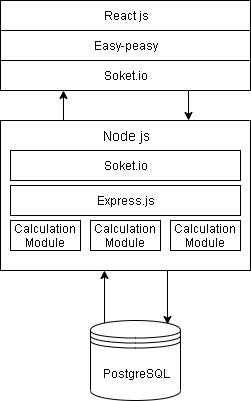
\includegraphics[scale=0.7]{my_folder/images/application architecture}
	\caption{Архитектура приложения}
	\label{fig:АpplicationАrchitecture}
\end{figure}

При подробном рассмотрении Рис. \ref{fig:АpplicationАrchitecture}, как ранее было сказано, библиотека React представляет клиентскую часть. Она обеспечивает масштабируемую разработку пользовательского интерфейса. Централизованное хранение информации реализовано с помощью библиотеки Easy-peasy. Она представляет информацию в виде глобального объект-хранилища. Взаимодействие с серверной частью происходит в рамках классического RESTful API. Реализовано с помощью отправки со стороны клиента Ajax-запросов, которые реализованы в Socket.io. Так же сам трансфер данных реализован с помощью Socket.io в рамках шаблона проектирования «издатель-подписчик». Это позволяет клиенту передавать данные заезда парусной яхты для расчёта отчётов на серверной стороне, которые он сохраняет в базе данных и отправляет обработанные данные клиенту для формирования отчётов на клиентской стороне. Для взаимодействия с PostgreSQL используется модуль pg\cite{pgnpm78:online} (неблокирующий клиент PostgreSQL для Node.js, не требующий дополнительных библиотек), позволяющий производить манипуляцию данных между базой данных и сервером. При получении данных на сервер определенного типа о необходимости расчёта данных, первоначально осуществляется поиск уже обработанных данных в СУБД PostgreSQL. Если же данные не найдены, то осуществляется расчёт отправленных пользователем данных. 

На Рис. \ref{fig:rgt_startReport} представлен пользовательский интерфейс приложения, разработанный с помощью Material-UI, а так же отчёт по Start report, показывающий инфографику начала стартового пути яхты.






\begin{figure}[hb]
	\centering
	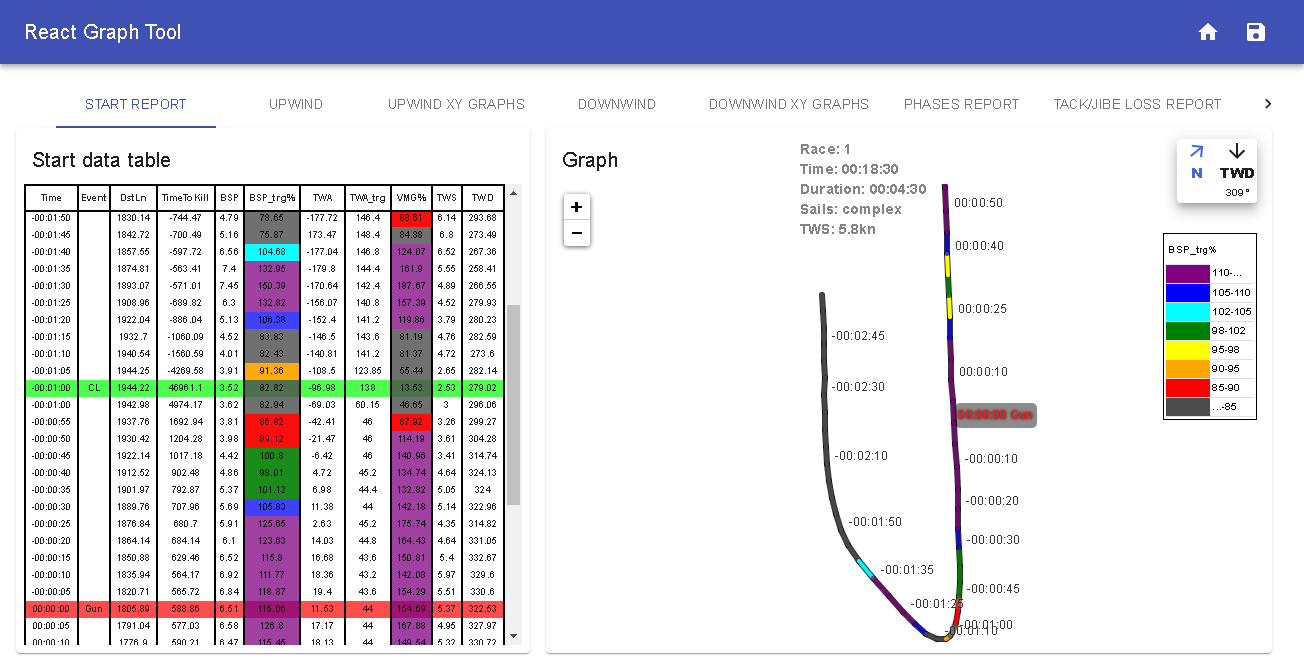
\includegraphics[scale=0.35]{my_folder/images/rgt_startReport}
	\caption{Пользовательский интерфейс вкладки Start report}
	\label{fig:rgt_startReport}
\end{figure}


На Рис. \ref{fig:rgt_XY} представлен, разработанный Upwind xy report, инфографику показывающие отношение характеристик к угловому ветру с помощью Material-UI.

\begin{figure}
	\centering
	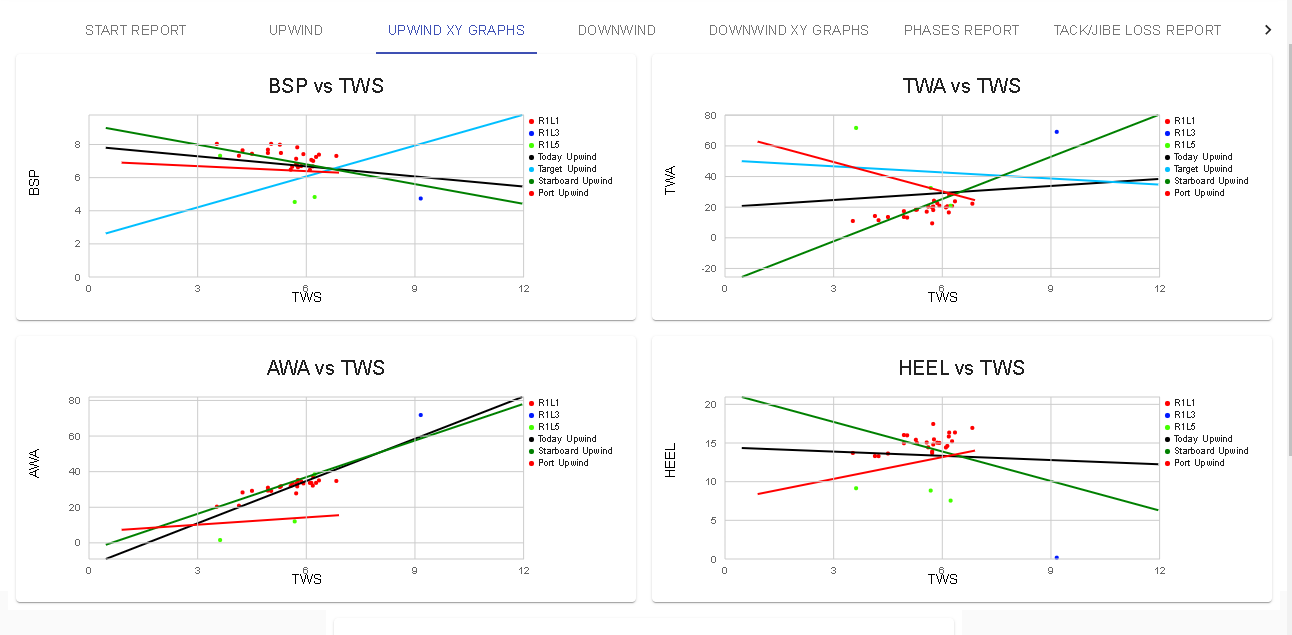
\includegraphics[scale=0.35]{my_folder/images/rgt_XY}
	\caption{Upwind XY report}
	\label{fig:rgt_XY}
\end{figure}

На Hис.\ref{fig:easypeasy} представлен срез глобального хранилища Easy-peasy.

\begin{figure}
	\centering
	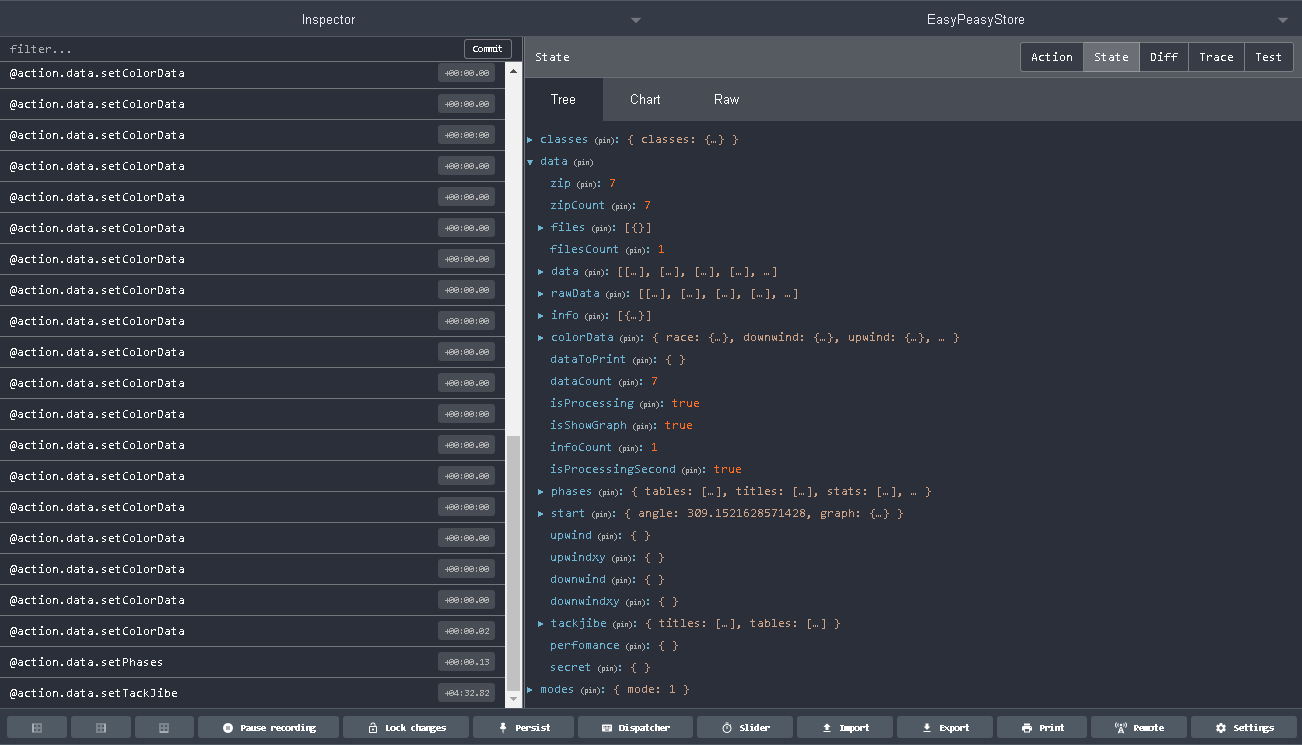
\includegraphics[scale=0.35]{my_folder/images/easypeasy}
	\caption{Upwind XY report}
	\label{fig:easypeasy}
\end{figure}

Приложения \cite{appendix:RGTMapGraph,appendix:RGTTableGraph,appendix:ReliseRESTfulAPI} демонстрируют код моделей табличного представления данных, графа пути. 

\newpage

\section{Сравнение с существующими технологиями} \label{ch3:sec5}

Тестирование прототипа реализовано с помощью фреймворка для нагрузочного тестирования Artillery.io. Он позволяет писать сценарии взаимодействия с приложением, а так же имитировать сложное поведение пользователя посредством нескольких шагов и транзакций с помощью циклов, условий на коде Javascript. Artillery.io удобно использовать для отладки сложных приложений, таких как транзакционные API, бэкэнд IoT,, бэкэнды онлайн игр и все виды сервисов с отслеживанием состояния.

Artillery.io обладает широким функционалом, который позволяет оценить время отклика, время задержки, количество запросов в секунду или отслеживать кастомные показатели с помощью кода Javascript.

Пример одного из использованных пользовательских сценариев показан:

\begin{lstlisting}
{
config:
	  target: "https://localhost:3000"
	  phases:
	- duration: 1000
		  arrivalRate: 1 
	  payload:
		  path: "Report_2020_05_13_11_59_01.fsr"
		  fields:
			- "files"
scenarios:
	- name: "Show start graph"
	  flow:
		- post:
			  url: "/api/start-report"
			  body: "file={{ keywords }}"
		- get:
			  url: "/start-report"
		- think: 500
\end{lstlisting}

Каждую секунду в течение 1000 секунд новый виртуальный пользователь отправляет файл из поля fields.file, пост запросом, на отображение стартовой страницы и остаётся в открытом соединении в течение 500 секунд.

Artillery.io предоставляет множество метрик для оценки тестов. Одни из них - количество выполненных запросов. Они являются количеством отправленных HTTP-запросов и ответов или сообщений от WebSocket. Так же число отправленных запросов в секунду. Является средним количеством запросов в секунду, выполненных за предыдущие 10 секунд (или в течение всего теста). Задержка запроса в миллисекундах. Значения p95 и p99, которые показывают максимальный предел задержки у 99 и 95 соответственно процентов запросов (к примеру, для 95 - показывает, что из 100 запросов 95-и запросам потребовалось меньше или равное 450мс).

Для сравнения с аналогами было принято решение использовать фреймворк artillery.io для проведения нагрузочного тестирования приложений B\&G sailing features и Sailwave на основе API Pusher.

\begin{table}
	\caption{Результаты нагрузочного тестирования}
	\label{loadTestResult}
	\begin{tabularx}{\linewidth}{|X|X|X|X|X|X|}
		\hline
		& Request latency (min) & Request latency (max) & Request latency (median) & P95 & P99\\
		\hline
		B\&G sailing features & 121 мс & 135 мс & 127 мс & 123 мс & 133 мс \\
		\hline
		Sailwave & (только Desktop) & (только Desktop) & (только Desktop) & (только Desktop) & (только Desktop)\\
		\hline
		Прототип приложения & 128 мс & 169 мс & 143 мс & 132 мс & 144 мс\\
		\hline
	\end{tabularx}
\end{table}

\begin{table}
	\caption{Таблица сравнения программ}
	\label{TableOfCmpPrograms}
	\begin{tabularx}{\linewidth}{|X|X|X|X|}
		\hline
		& Вид распространения & Цена & Функционал\\
		\hline
		B\&G sailing features & Desktop/ lite web & От 700\$ и может больше 2000\$ в зависимости от решения & Start report,
		Phase report,
		XY report,
		Tack/Jibe Loss report\\
		\hline
		Sailwave & Desktop & Free &Phase report,
		XY report,
		Tack/Jibe Loss report\\
		\hline
		Прототип приложения & web & Free & Start report,
		Phase report,
		XY report,
		Tack/Jibe Loss report,
		Perfomances\\
		\hline
	\end{tabularx}
\end{table}

\newpage

\section{Выводы} \label{ch3:conclusion}

В данной главе была сформулирована методика, предполагающая выполнение последовательности действий для сокращения угроз. Так же был определен стек для разработки прототипа приложения. Прототип специализированного веб-приложения для формирования отчётов по данным с заездов парусных яхт в период тренировок был разработан. Так же данный прототип подвергся нагрузочному тестированию. Были созданы тесты, которые имитируют посещение веб-приложения виртуальными пользователями. Нагрузочное тестирование показало, что прототип уступает по показателям, однако результаты можно считать сопоставимыми с результатами коммерческие аналогов, из чего следует, что предложенный архитектурный подход можно считать приемлемым.


%% Вспомогательные команды - Additional commands
%
%\newpage % принудительное начало с новой страницы, использовать только в конце раздела
%\clearpage % осуществляется пакетом <<placeins>> в пределах секций
%\newpage\leavevmode\thispagestyle{empty}\newpage % 100 % начало новой страницы           	 % Глава 3
\chapter{Название четвёртой главы. Апробация результатов исследования, а~именно: метода, алгоритма, модели исследования} \label{ch4}

% не рекомендуется использовать отдельную section <<введение>> после лета 2020 года
%\section{Введение} \label{ch4:intro}

Хорошим стилем является наличие введения к главе. Во введении может быть описана цель написания главы, а также приведена краткая структура главы. 
	
\section{Название параграфа} \label{ch4:sec1}

\section{Название параграфа} \label{ch4:sec2}

Пример ссылки на литературу \cite{avtonomova:fya,Peskov2004-ru,Kotelnikov2004-ru,Kotelnikov2004}.

%\FloatBarrier % заставить рисунки и другие подвижные (float) элементы остановиться

\section{Выводы} \label{ch4:conclusion}

Текст выводов по главе \thechapter.

%% Вспомогательные команды - Additional commands
%
%\newpage % принудительное начало с новой страницы, использовать только в конце раздела
%\clearpage % осуществляется пакетом <<placeins>> в пределах секций
%\newpage\leavevmode\thispagestyle{empty}\newpage % 100 % начало новой страницы           	 % Глава 3
\ContinueChapterEnd % завершить размещение глав <<подряд>>
%% Завершение основной части

\chapter*{Заключение} \label{ch-conclusion}
\addcontentsline{toc}{chapter}{Заключение}	% в оглавление 

В первой главе была произведена классификация highload приложений и они были определены. Были представлены направления, в которых используется высоконагруженные системы и примеры таких систем. Были проанализированы актуальные угрозы веб-приложений, а так же методы борьбы с ними.

Во второй главе были определены тип веб-приложения, ключевые ресурсы веб-приложений и виды хостинга. Кроме того, были проанализированы виды транспорта передачи данных с описанием достоинства и недостатков каждого. Были определены инструменты для построения таких веб-приложений. Было проведено исследование задержки реакции системы при разработке используя стандартный протокол WebSocket, Socket.io и SockJS. Проведён эксперимент по замеру времени передачи сообщения. 

В данной главе была сформулирована методика, предполагающая выполнение последовательности действий для сокращения угроз. Так же был определен стек для разработки прототипа приложения. Прототип специализированного веб-приложения для формирования отчётов по данным с заездов парусных яхт в период тренировок был разработан. Так же данный прототип подвергся нагрузочному тестированию. Были созданы тесты, которые имитируют посещение веб-приложения виртуальными пользователями. Нагрузочное тестирование показало, что прототип уступает по показателям, однако результаты можно считать сопоставимыми с результатами коммерческие аналогов, из чего следует, что предложенный архитектурный подход можно считать приемлемым.

На основании данных результатов, можно утверждать, что прототип веб-приложения, реализованный в рамках методики может составить конкуренцию аналогичным коммерческим продуктам, так как  является более предпочтительным по некоторым аспектам, например, из-за цены такого подхода.

        	 % Заключение

%% Наличие следующих перечней не исключает расшифровку сокращения и условного обозначения при первом упоминании в тексте!
\chapter*{Список сокращений и условных обозначений}             % Заголовок
\addcontentsline{toc}{chapter}{Список сокращений и условных обозначений}  % Добавляем его в оглавление
\noindent
\addtocounter{table}{-1}% Нужно откатить на единицу счетчик номеров таблиц, так как следующая таблица сделана для удобства представления информации по ГОСТ
%\begin{longtabu} to \dimexpr \textwidth-5\tabcolsep {r X}
\begin{longtabu} to \textwidth {r X} % Таблицу не прорисовываем!
% Жирное начертание для математических символов может иметь
% дополнительный смысл, поэтому они приводятся как в тексте
% диссертации
\textbf{DOI} & Digital Object Identifier. \\
\textbf{WoS} & Web of Science. \\
\textbf{ВКР}  & Выпускная квалификационная работа. \\
\textbf{ТГ-объект}  & Текстово-графический объект. \\
\textbf{APM} & Application Performance Monitoring \\
%$\begin{rcases}
%a_n\\
%b_n
%\end{rcases}$  & 
%\begin{minipage}{\linewidth}
%Коэффициенты разложения Ми в дальнем поле, соответствующие
%электрическим и магнитным мультиполям.
%\end{minipage}
%\\
%${\boldsymbol{\hat{\mathrm e}}}$ & Единичный вектор. \\
%$E_0$ & Амплитуда падающего поля.\\
%$\begin{rcases}
%a_n\\
%b_n
%\end{rcases}$  & 
%Коэффициенты разложения Ми в дальнем поле соответствующие
%электрическим и магнитным мультиполям ещё раз, но без окружения
%minipage нет вертикального выравнивания по центру.
%\\
%$j$ & Тип функции Бесселя.\\
%$k$ & Волновой вектор падающей волны.\\
%
%$\begin{rcases}
%a_n\\
%b_n
%\end{rcases}$  & 
%\begin{minipage}{\linewidth}
%\vspace{0.7em}
%Коэффициенты разложения Ми в дальнем поле соответствующие
%электрическим и магнитным мультиполям, теперь окружение minipage есть
%и добавленно много текста, так что описание группы условных
%обозначений значительно превысило высоту этой группы... Для отбивки
%пришлось добавить дополнительные отступы.
%\vspace{0.5em}
%\end{minipage}
%\\
%$L$ & Общее число слоёв.\\
%$l$ & Номер слоя внутри стратифицированной сферы.\\
%$\lambda$ & Длина волны электромагнитного излучения
%в вакууме.\\
%$n$ & Порядок мультиполя.\\
%$\begin{rcases}
%{\mathbf{N}}_{e1n}^{(j)}&{\mathbf{N}}_{o1n}^{(j)}\\
%{\mathbf{M}_{o1n}^{(j)}}&{\mathbf{M}_{e1n}^{(j)}}
%\end{rcases}$  & Сферические векторные гармоники.\\
%$\mu$  & Магнитная проницаемость в вакууме.\\
%$r,\theta,\phi$ & Полярные координаты.\\
%$\omega$ & Частота падающей волны.\\
%
%  \textbf{BEM} & Boundary element method, метод граничных элементов.\\
%  \textbf{CST MWS} & Computer Simulation Technology Microwave Studio.
\end{longtabu}
		         % Необязательная рубрика! Список сокращений и условных обозначений

\chapter*{Словарь терминов}             % Заголовок
\addcontentsline{toc}{chapter}{Словарь терминов}  % Добавляем его в оглавление

\textbf{TeX} --- язык вёрстки текста и издательская система, разработанные Дональдом Кнутом.

\textbf{LaTeX} --- язык вёрстки текста и издательская система, разработанные Лэсли Лампортом как надстройка над TeX.

    		 % Необязательная рубрика! Словарь терминов
% По порядку после Списка сокращений и условных обозначений, если есть.	


%%% Не мянять - Do not modify
%%
%%
\clearpage                                  % В том числе гарантирует, что список литературы в оглавлении будет с правильным номером страницы
%\hypersetup{ urlcolor=black }               % Ссылки делаем чёрными
%\providecommand*{\BibDash}{}                % В стилях ugost2008 отключаем использование тире как разделителя 
\urlstyle{rm}                               % ссылки URL обычным шрифтом
\ifdefmacro{\microtypesetup}{\microtypesetup{protrusion=false}}{} % не рекомендуется применять пакет микротипографики к автоматически генерируемому списку литературы
%\newcommand{\fullbibtitle}{Список литературы} % (ГОСТ Р 7.0.11-2011, 4)
%\insertbibliofull  
%\noindent
%\begin{group}
\chapter*{Список использованных источников}	
\label{references}
\addcontentsline{toc}{chapter}{Список использованных источников}	% в оглавление 
\printbibliography[env=SSTfirst]                         % Подключаем Bib-базы
%\ifdefmacro{\microtypesetup}{\microtypesetup{protrusion=true}}{}
%\urlstyle{tt}                               % возвращаем установки шрифта ссылок URL
%\hypersetup{ urlcolor={urlcolor} }          % Восстанавливаем цвет ссылок



%\urlstyle{rm}                               % ссылки URL обычным шрифтом
%\ifdefmacro{\microtypesetup}{\microtypesetup{protrusion=false}}{} % не рекомендуется применять пакет микротипографики к автоматически генерируемому списку литературы
%\insertbibliofull                           % Подключаем Bib-базы
%\ifdefmacro{\microtypesetup}{\microtypesetup{protrusion=true}}{}
%\urlstyle{tt}                               % возвращаем установки шрифта ссылок URL
		     % Список литературы

% Здесь можно поместить список иллюстративного материала

\appendix % не редактировать / keep unmodified


%\chapter{Фрагменты исходного кода}\label{appendix-MikTeX-TexStudio}		


\chapter{Реализация метода анализа иерархий (Саати)}
\label{appendix:methodSaati}
Листинг кода метода Саати для выбора наилучшего решения из представленных вариантов по заданным критериям.

\textit{main.py:}
\begin{lstlisting}[breaklines]
import json
import my_math as math

model_tmp_table = {}
text = ''

with open('model2.json') as json_model:
# model can also be a python dictionary
model = json.load(json_model)

text = math.makeSignificanceTable(model_tmp_table, model, text)
text = math.makeOptionMatrixTables(model_tmp_table, model, text)
text = math.makeFinaleMatrix(model_tmp_table, model, text)

answer = model_tmp_table['result']

list_d = list(answer.items())
list_d.sort(key=lambda i: i[1])
last_item = len(list_d)-1

for i in list_d:
print('{0:<10} : {1:^7f}'.format(i[0],i[1]))
text += '{0:<10} : {1:^7f}'.format(i[0],i[1]) + "\n"

print('\nBest item is => {:<20}'.format(list_d[last_item][0]))
text += '\nBest item is => {:<20}'.format(list_d[last_item][0])

f= open("result.txt","w+")

f.write(text)
f.close()

my_math.py:
import numpy as np
import json
import copy

def format_matrix(header, matrix, top_format, left_format, cell_format, row_delim, col_delim, val, kek = False, pos = 0):

if(kek):
header.insert(pos, "")
for i in matrix:
i.insert(pos, "")

table = [[''] + header] + [[name] + row for name, row in zip(header, matrix)]
if(kek):
table_format = [['{:^{}}'] + len(header) * [top_format]] + (len(matrix)  - 2 + val) * [[left_format] + (len(header) - 3) * [cell_format] + ['{}'] + 2 * [cell_format]]
else:
table_format = [['{:^{}}'] + len(header) * [top_format]] + (len(matrix)  - 2 + val) * [[left_format] + len(header) * [cell_format]]
col_widths = [max(len(format.format(cell, 0)) for format, cell in zip(col_format, col))for col_format, col in zip(zip(*table_format), zip(*table))]
return row_delim.join(col_delim.join(format.format(cell, width) 
for format, cell, width in zip(row_format, row, col_widths)) 
for row_format, row in zip(table_format, table))



def makeSignificanceTable(model_tmp_table, model, my_str): # Second level matrix
significance_table = {}
criteria = model['criteria']
for idx1, key1 in enumerate(criteria):
row = []
for idx2, key2 in enumerate(criteria):
row.append(criteria[key1]/criteria[key2])
significance_table[key1] = row

for row in significance_table:
tmp = 1
for j in significance_table[row]:
tmp *= j
tmp = tmp**(1./len(significance_table[row]))
significance_table[row].append(tmp)

tmp = 0
for row in significance_table:
tmp += significance_table[row][len(significance_table[row]) - 1]
check = 0

length = len(list(significance_table.values())[0]) - 1
for row in significance_table:
significance_table[row].append(significance_table[row][length] / tmp)
check += significance_table[row][length + 1]

str = 'Significance Table'
print("\n"+"#"*(6 + len(str))+"\n\n   " + str + "\n\n"+"#"*(6 + len(str)))
my_str += "\n"+"#"*(6 + len(str))+"\n\n   " + str + "\n\n"+"#"*(6 + len(str)) + "\n"
header = [key for key in significance_table]
matrix = [significance_table[key] for key in significance_table]
print(format_matrix(header, matrix, '{:^{}}', '{:<{}}', '{:>{}.5f}', '\n', ' | ', 2))
my_str += format_matrix(header, matrix, '{:^{}}', '{:<{}}', '{:>{}.5f}', '\n', ' | ', 2) + "\n\n\n"

print("\n\n")

model_tmp_table['significance_criteria'] = significance_table
return my_str


def makeOptionMatrixTables(model_tmp_table, model, my_str): # Third level matrixs
matrix = {}
matrix_by_options = model['options']
criteria_names = model['criteria'].keys()
tmp_list = matrix_by_options.values()
length = len(list(tmp_list)[0])	

for i in range(length):
table = []
for idx1, key1 in enumerate(matrix_by_options):
row = []
for idx2, key2 in enumerate(matrix_by_options):
row.append(matrix_by_options[key1][i] / matrix_by_options[key2][i])
table.append(row)

matrix[list(criteria_names)[i]] = table

for idx, key in enumerate(matrix):
table = matrix[key]
for row in table:
tmp = 1
for j in row:
tmp *= j
tmp = tmp**(1./len(row))
row.append(tmp)

for idx, key in enumerate(matrix):
tmp = 0
for row in matrix[key]:
tmp += row[len(row) - 1]
check = 0
length = len(matrix[key][0]) - 1
for row in matrix[key]:
row.append(row[length] / tmp)
check += row[length + 1]

str1 = 'Tables of significant factors for each criterion'
print("\n"+"#"*(6 + len(str1))+"\n\n   " + str1 + "\n\n"+"#"*(6 + len(str1)))
my_str += "\n"+"#"*(6 + len(str1))+"\n\n   " + str1 + "\n\n"+"#"*(6 + len(str1)) + "\n"
header = [key for key in matrix_by_options]

for key in matrix:
print("\n\tBy "+ key)
my_str += "\n\tBy "+ key + "\n"
tmp = 0
for row in matrix[key]:
tmp += row[len(row) - 1]
check = 0
length = len(matrix[key][0]) - 1
for row in matrix[key]:
row.append(row[length] / tmp)
check += row[length + 1]
answ = format_matrix(copy.deepcopy(header) + ["Weight", "% of importance"], copy.deepcopy(matrix[key]) , '{:^{}}', '{:<{}}', '{:>{}.5f}', '\n', ' | ', 2, True, len(header))
print(answ)
my_str += answ + "\n"
print("SUM %: ", check)
my_str += "SUM %: " + str(check) + "\n"
print("\n\n")
model_tmp_table['matrix_by_criteria'] = matrix
return my_str


def makeFinaleMatrix(model_tmp_table, model, my_str): # Final result
final = []
for_multiply = model_tmp_table["significance_criteria"]
conclusion = model_tmp_table["matrix_by_criteria"]

str = 'Final matrix for calculating weights for each element'

fin_answ_tab = "\n"+"#"*(6 + len(str))+"\n\n   " + str + "\n\n"+"#"*(6 + len(str)) + "\n\n"

header = [key for idx, key in enumerate(conclusion)]
str_leng = max([len(key) for idx, key in enumerate(conclusion)])
ttt = max([len(key) for idx, key in enumerate(model['options'])])
str_leng = max(str_leng, ttt)
str_leng =  8 if str_leng<8 else str_leng
side = [key for idx, key in enumerate(model['options'])]
side.insert(0, " " * str_leng)

for i, row in enumerate(side):
if i == 0:
for idx, key in enumerate(conclusion):
row += "|"
row += "{name:<{size}}".format(name=key, size=str_leng)
row += "|" +  "{name:<{size}}".format(name="% weight", size=str_leng) + "\n"
row += "-" * str_leng + "|" + "|".join([("-" * str_leng) for i in range(len(conclusion) + 1)]) + "\n"
else:
row = "{name:<{size}}".format(name=row, size=str_leng)
summ_to_final = 0
for idx, key in enumerate(conclusion):
summ_to_final += copy.deepcopy(conclusion[key][i-1]).pop() * copy.deepcopy(for_multiply[key]).pop()
row += "|" + "{name:>{size}.5f}".format(name=copy.deepcopy(conclusion[key][i-1]).pop(), size=str_leng)

row += "|" + "{name:>{size}.5f}".format(name=summ_to_final, size=str_leng) +"\n" 
fin_answ_tab += row
fin_answ_tab += "-" * str_leng + "|" + "|".join([("-" * str_leng) for i in range(len(conclusion))]) + "|" + "\n"
fin_answ_tab += "{name:^{size}}".format(name="SP", size=str_leng) + "|"
for i, key in enumerate(for_multiply): 
fin_answ_tab += "{name:>{size}.5f}".format(name=copy.deepcopy(for_multiply[key]).pop(), size=str_leng) + "|"

fin_answ_tab += "\n\n\t Where SP - the significance of the criterion\n\n"
print(fin_answ_tab)
for idx, key in enumerate(conclusion):
row = []
length = len(for_multiply[key]) - 1
for i in conclusion[key]:
row.append(i[len(i)-1] * for_multiply[key][length])
final.append(row)

arr1 = np.array(final)
arr1_transpose = arr1.transpose()
okey = {}
x = iter(list(model["options"].keys()))
for i in arr1_transpose:
k = next(x)
okey[k] = sum(i)

model_tmp_table['result'] = okey
return my_str + fin_answ_tab
\end{lstlisting}

\chapter{Расчёт наилучшего транспорта передачи данных} \label{appendix:calculBestTransferDataWay}

Зададим значимость к критерия для расчётов. Количество запросов  на опрос сервера (Cnt req on poll): 4. Количество служебных заголовков вместе с ответом (Cnt of serv head): 3. Служебная информация прикрепляемая в ответе и запросе (Service info): 5. Согласно \taref{comparisonOfTypesOfDataTransmission}, модель соответствия вариантов критериям имеет следующие значения:

\begin{lstlisting}
{
	"name": "Choose transfer data",
	"criteria": { 
		"Cnt req on poll"		: 4,
		"Cnt of serv head"	: 3,
		"Service info"			: 5
	},
	"options": {
		"WebSockets"         :   [4, 4, 5],
		"Server-sent events" :   [4, 4, 4],
		"Long Polling"       :   [4, 3, 2],
		"Ajax Polling"       :   [3, 3, 2]
	} 
}
\end{lstlisting}

Расчёт наилучшего решения приведённой модели из Приложения \ref{appendix:methodSaati}:

\begin{figure}
	\centering
	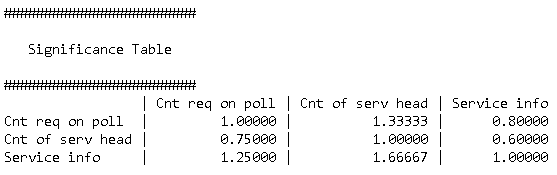
\includegraphics[width=1\linewidth]{my_folder/images/ATransferData1}
	\caption{Таблица значимости}
	\label{fig:atransferdata1}
\end{figure}

\begin{figure}
	\centering
	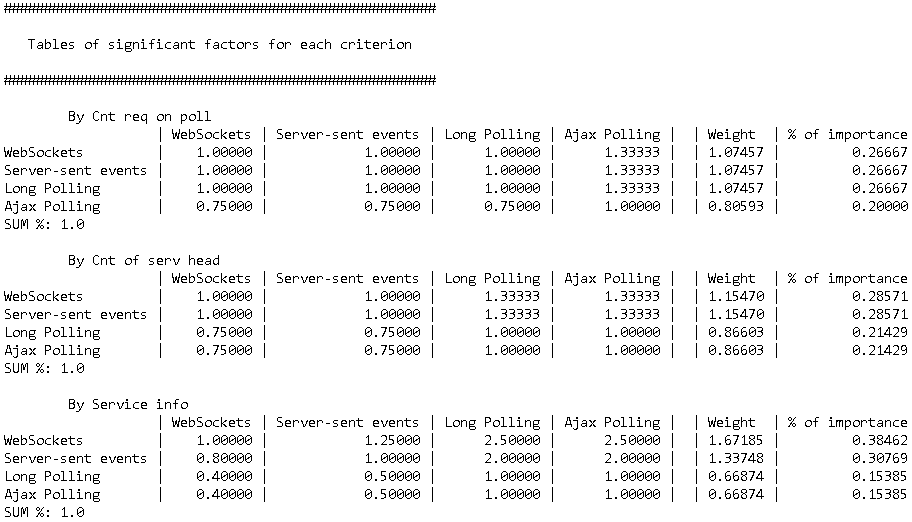
\includegraphics[scale=0.7, angle=270]{my_folder/images/ATransferData2}
	\caption{Таблицы значимых факторов для каждого критерия}
	\label{fig:atransferdata2}
\end{figure}

\begin{figure}
	\centering
	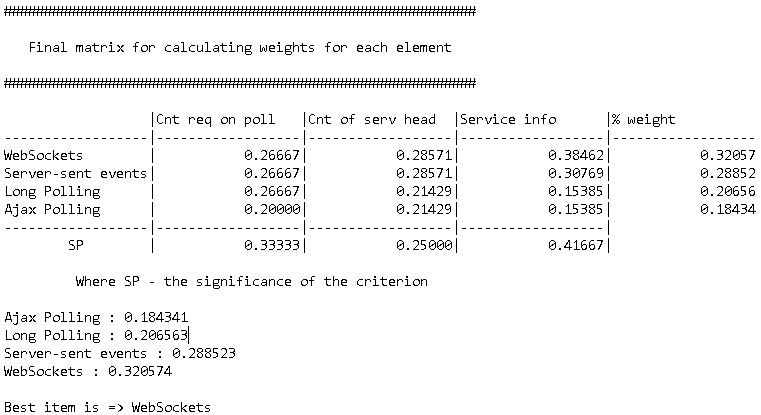
\includegraphics[width=1\linewidth]{my_folder/images/ATransferData3}
	\caption{Результируюящя таблица}
	\label{fig:atransferdata3}
\end{figure}


\chapter{Сравнение выполнения одинаковых задач разными языками программирования}
\label{appendix:comparationPL}

Данная таблица построена на основе данных с электронного ресурса \cite{\ref{appendix:methodSaati}} . Цветовая идентификация имеет следующий характер: Насыщенный зелёный – самый лучший результат, зелёный – второй лучший результат, оранжевый – самый худший результат.

\begin{table}
	\caption{Список угроз с основными методами противодействия им}
	\label{listOfRisk232}
	\centering
	\begin{tabularx}{\linewidth}{p{4.5cm}cccc}
		& PHP & Node js & Java & Python \\
		regex-redux & \cellcolor[rgb]{0.76,0.84,0.61} 2,88 & 9,53 & \cellcolor[rgb]{0.89,0.42,0.04} 10,27 & \cellcolor[rgb]{0.57,0.82,0.31} 2,67 \\
		pidigits & \cellcolor[rgb]{0.76,0.84,0.61} 2,11 & \cellcolor[rgb]{0.89,0.42,0.04} 2,58 & \cellcolor[rgb]{0.57,0.82,0.31}  1,83 & 2,39 \\
		k-nucleotide & 41,32 & \cellcolor[rgb]{0.76,0.84,0.61} 26,32 & \cellcolor[rgb]{0.57,0.82,0.31} 9,14 & \cellcolor[rgb]{0.89,0.42,0.04} 72,58 \\
		binary-trees & 51,13 & \cellcolor[rgb]{0.76,0.84,0.61} 19,22 & \cellcolor[rgb]{0.57,0.82,0.31} 8,28 & \cellcolor[rgb]{0.89,0.42,0.04} 80,82 \\
		reverse-complement & 14,19 & \cellcolor[rgb]{0.76,0.84,0.61} 4,1 & \cellcolor[rgb]{0.57,0.82,0.31} 3,27 & \cellcolor[rgb]{0.89,0.42,0.04} 16,41 \\
		spectral-norm & 33,24 & \cellcolor[rgb]{0.76,0.84,0.61} 4,4 & \cellcolor[rgb]{0.57,0.82,0.31} 4,15 & \cellcolor[rgb]{0.89,0.42,0.04} 170,1 \\
		fannkuch-redux & 219,15 & \cellcolor[rgb]{0.76,0.84,0.61} 19,48 & \cellcolor[rgb]{0.57,0.82,0.31} 16,12 & \cellcolor[rgb]{0.89,0.42,0.04} 494,58 \\
		n-body & 329,52 & \cellcolor[rgb]{0.76,0.84,0.61} 26,28 & \cellcolor[rgb]{0.57,0.82,0.31} 21,85 & \cellcolor[rgb]{0.89,0.42,0.04} 891,12 \\
		fasta & 53,24 & \cellcolor[rgb]{0.76,0.84,0.61} 3,62 & \cellcolor[rgb]{0.57,0.82,0.31} 2,22 & \cellcolor[rgb]{0.89,0.42,0.04} 63,63 \\
		mandelbrot & 105,4 & \cellcolor[rgb]{0.57,0.82,0.31} 6,84 & \cellcolor[rgb]{0.57,0.82,0.31} 6,84 & \cellcolor[rgb]{0.89,0.42,0.04} 263,87 \\
	\end{tabularx}
\end{table}

\chapter{Выбор серверного языка}
\label{appendix:choosingServerSideLanguage}

Зададим значимость к критерия для расчётов. Согласно Таблица \ref{comparisonOfProgrammingLanguage}., модель соответствия вариантов критериям имеет следующие значения:

\begin{lstlisting}
{
	"name": "Choose best language",
	"criteria": { 
		"Libraries"	: 4,
		"DB"				: 3,
		"Speed"			: 5,
		"Framework"	: 4
	},
	"options": {
		"Python"	:   [5, 3, 3, 4],
		"Node Js"	:   [5, 4, 4, 5],
		"Java"		:   [4, 5, 5, 4],
		"PHP"			:   [4, 4, 4, 4]
	} 
}
\end{lstlisting}

Расчёт наилучшего решения приведённой модели с Приложение \ref{appendix:methodSaati}

\begin{figure}
	\centering
	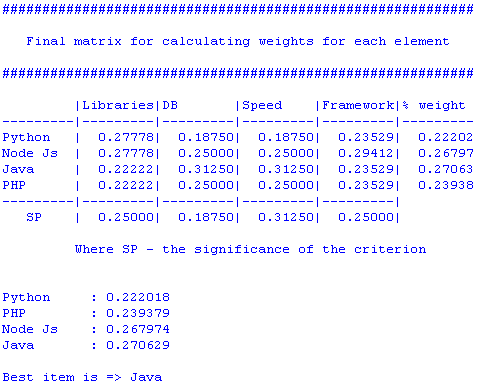
\includegraphics[width=1\linewidth]{my_folder/images/BestSolution1}
	\caption{Результирующая таблица}
	\label{fig:BestSolution1}
\end{figure}

\chapter{Реализация серверной части Socket.io}
\label{appendix:serverSideBySocketIO}

Листинг программного кода серверной части на Node.js, Express.js и Socket.io, для анализа библиотек.


\begin{lstlisting}
const path = require('path');
const express = require('express');

const port = process.env.PORT || 80;
const app = express();
const server = require('http').Server(app); 
const socketio = require('socketio')(server);

const uuid = require('uuid/v4');
const createCsvWriter = require('csv-writer').createObjectCsvWriter; const csvWriter = createCsvWriter({
path: 'stats-si.csv',
header: [
{id: 'msg', title: 'MSG'},
{id: 'id', title: 'UUID'},
{id: 'tmspStart', title: 'TMPSTART'},
{id: 'tmspEnd', title: 'TMPEND'}
] 
});
const messageCount = 1000;
const stats = new Map();

io.on('connection', socket => {
for (let t = 0; t < messageCount; t++) {
const id = uuid();
const sendedMsg = { msg: 'ping', id, tmspStart: Date.now(), tmspEnd: ''};
stats.set(sendedMsg.id, sendedMsg); io.sockets.emit('message', JSON.stringify(sendedMsg));
}

socket.on('message', (message) => {
if (counter < messageCount) {
counter++;
} else {
io.close();
}
const parsedMsg = JSON.parse(message);
parsedMsg.tmspEnd = Date.now();
parsedMsg.msg = "roundtrip";
parsedMsg.tmspStart; stats.set(parsedMsg.id, parsedMsg);
});

socket.on('disconnect', () => {
const records = Array.from(stats, keyValuePair => keyValuePair[1]);
csvWriter.writeRecords(records)
.then(() => {
})
.catch((err) => { console.log(err) });
})
});

app.get('/', function (req, res) {
res.sendFile(path.resolve('../index.html'));
});

server.listen(port, () => console.log(`Listening on port ${port}`));
\end{lstlisting}

\chapter{Реализация серверной части SockJS}
\label{appendix:serverSideBySockJS}

Листинг программного кода серверной части на Node.js, Express.js и Socket.io, для анализа библиотек.

\begin{lstlisting}
const http = require('http');
const sockjs = require('sockjs');
const node_static = require('node-static'); 
const path = require('path'); const fs = require("fs");
const uuid = require('uuid/v4');
const createCsvWriter = require('csv-writer').createObjectCsvWriter; const csvWriter = createCsvWriter({
path: 'stats-sk.csv',
header: [
{id: 'msg', title: 'MSG'},
{id: 'id', title: 'UUID'},
{id: 'tmspStart', title: 'TMPSTART'},
{id: 'tmspEnd', title: 'TMPEND'}
]
});

const sockjs_opts = {
prefix: '/echo'
};

const port = 80;
const messageCount = 1000;
let counter = 0;
const stats = new Map();
const sockjs_echo = sockjs.createServer(sockjs_opts); sockjs_echo.on('connection', function(conn) {
for (let t = 0; t < messageCount; t++) {
const id = uuid();
const sendedMsg = { msg: 'ping', id, tmspStart: Date.now(), tmspEnd: ''};
stats.set(sendedMsg.id, sendedMsg);
conn.write(JSON.stringify(sendedMsg));
}
conn.on('data', (message) => {
if (counter < messageCount) {
counter++;
} else {
conn.close();
}
const parsedMsg = JSON.parse(message);
parsedMsg.tmspEnd = Date.now();
parsedMsg.msg = "roundtrip";
stats.set(parsedMsg.id, parsedMsg);
});
conn.on('close', function() {
console.log('connection is closed');
const records = Array.from(stats, keyValuePair => keyValuePair[1]);
csvWriter.writeRecords(records);
});
});

const static_directory = new node_static.Server(path.resolve('../test-ws/client/index-sk.html'));

const server = http.createServer(); server.addListener('request', function(req, res) {
static_directory.serve(req, res);
});

server.addListener('upgrade', function(req, res) { 
res.end();
});
sockjs_echo.installHandlers(server);
console.log(` Server listening on ${port}`);
server.listen(port, hostname);

\end{lstlisting}


\chapter{Выбор систему мониторинга}
\label{appendix:choosingMonitoringSys}

Зададим значимость к критерия для расчётов. Согласно Таблица \ref{comparisonOfAPM}., модель соответствия вариантов критериям имеет следующие значения:


\begin{lstlisting}
{
  "name": "Choose best APM",
  "criteria": { 
    "UI"                             : 3,
    "Distribution"                   : 4,
    "Tracing transaction"            : 5,
    "Correlation data"               : 3,
     "Support"                        : 4
  },
  "options": {
    "New Relic"     :   [5, 3, 4, 5, 5],
    "CloudWatch"    :   [3, 4, 1, 3, 3],
    "Dynatrace APM" :   [4, 5, 5, 5, 4],
    "AppDynamics"   :   [5, 5, 4, 4, 5],
    "CA APM"        :   [4, 5, 4, 5, 4]
 } 
}
\end{lstlisting}

Расчёт наилучшего решения приведённой модели с Приложение \ref{appendix:methodSaati}:

\begin{figure}
	\centering
	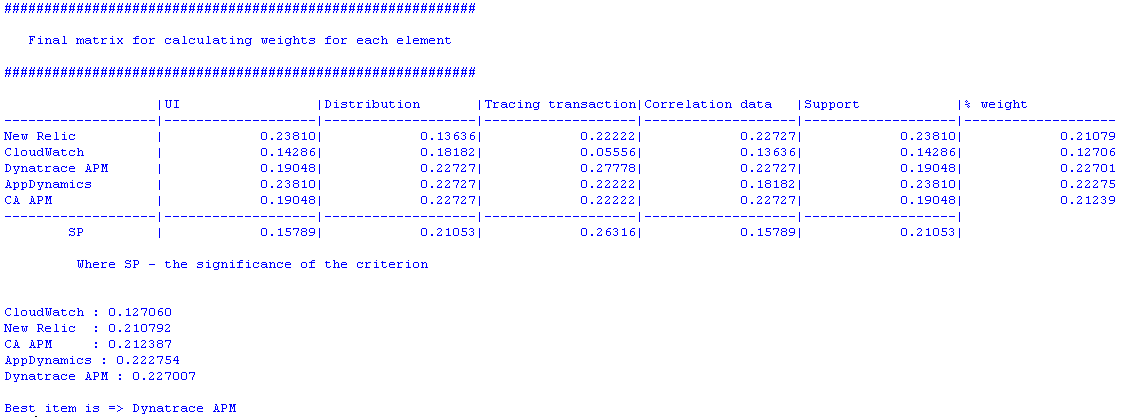
\includegraphics[width=1\linewidth]{my_folder/images/FMatrixMonitoringSys}
	\caption{Результирующая таблица}
	\label{fig:FMatrixMonitoringSys}
\end{figure}


\chapter{Компонента Map (граф)}
\label{appendix:RGTMapGraph}

Листинг кода реализации компоненты Map (граф начального пути яхты в start report)

\begin{lstlisting}
const MyMap = ({ graph, title, angle }) => {
const { classes } = useStoreState(state => state.classes);
const { rawData } = useStoreState(state => state.data);
const [lastZoom, changeLastZoom] = useState(0);
let heap = 0;
const mapRef = useRef(null);

const hideAndSeek = event => {
  let map = event.target;
  heap = 0;
  var zoom = map.getZoom();
  if (zoom < 16 && (!lastZoom || lastZoom >= 16)) {
    map.eachLayer(function(l) {
      if (l.getTooltip()) {
        var tooltip = l.getTooltip();
        l.unbindTooltip().bindTooltip(tooltip, {
          permanent: false
        });
      }
    });
  } else
  map.eachLayer(function(l) {
    if (l.getTooltip()) {
      var tooltip = l.getTooltip();
      l.unbindTooltip().bindTooltip(tooltip, {
        permanent: labelPermanent(tooltip.options.elevation, zoom)
      });
    }
  });

  changeLastZoom(zoom);
};

const labelPermanent = (wheight, zoom) => {
  let denominator = zoom - 16;
  let border = 320 / Math.pow(2, denominator);
  if (heap + wheight > border) {
    heap = 0;
    return true;
  } else {
    heap = heap + wheight;
    return false;
  }
};

const log = num => {
  return Math.log(num) / Math.log(2.0154);
};

const takeZoomLvl = () => {
  let zoomLvl = {
    x: [Math.min(...graph.x), Math.max(...graph.x)],
    y: [Math.min(...graph.y), Math.max(...graph.y)]
  };
  let y = Math.abs(zoomLvl.y[1] - zoomLvl.y[0]);
  let x = Math.abs(zoomLvl.x[1] - zoomLvl.x[0]);
  return Math.min(log(720 / x), log(360 / y));
};
return (
  <>
  {graph.hasOwnProperty("myGeoJSON") &&
  graph.hasOwnProperty("myGeoJSONLable") ? (
    <>
      <Legend />
      <Graphtitle tws={graph.tws} />
      <Arrow angle={angle} />
      {title && <Title title={title} />}
      <Map
        className={classes.mapLeaflet}
        id="leaflet-map"
        center={[graph.center[1], graph.center[0]]}
        useFlyTo={true}
        boundsOptions={{ padding: [25, 25] }}
        zoom={takeZoomLvl()}
        attributionControl={true}
        zoomControl={true}
        doubleClickZoom={true}
        scrollWheelZoom={true}
        dragging={true}
        maxZoom={20}
        minZoom={1}
        animate={true}
        easeLinearity={0.35}
        onZoomend={e => hideAndSeek(e)}
        ref={mapRef}
      >
        <TileLayer url="http://{s}.tile.osm.org/{z}/{x}/{y}.png" />
        {graph.geoJsonLines.features.map((feature, idx) => (
          <GeoJSON
            key={feature.key}
            data={feature}
            style={getStyle(feature.properties.name)}
          >
            {feature.properties.hasOwnProperty("point") ? (
              feature.properties.point.name.map((name, jdx) => (
                <Marker
                  position={feature.properties.point.coordinates[jdx]}
                  key={"SL-" + feature.properties.point.name[jdx]}
                >
                  <Tooltip
                    key={
                      "Tooltip-" + feature.properties.point.name[jdx] + jdx
                    }
                    direction="right"
                    offset={[-25, 15]}
                    elevation={feature.properties.point.elevation}
                    className={"tooltopSP"}
                    permanent={labelPermanent(
                    feature.properties.point.elevation,
                    takeZoomLvl()
                    )}
                  >
                    {feature.properties.point.name[jdx]}
                  </Tooltip>
                </Marker>
              ))
              ) : (
               <></>
              )}
          </GeoJSON>
        ))}
        {graph.myGeoJSON.features.map((feature, idx) => (
          <GeoJSON
            key={"lb- " + idx}
            data={feature}
            style={getStyle("black")}
          />
        ))}
        {graph.myGeoJSON.features.map((feature, idx) => (
          <GeoJSON
            key={"lf-" + idx}
            data={feature}
            style={getStyle(feature.properties.elevation)}
          />
        ))}
        {graph.myGeoJSONLable.map((feature, idx) => (
          <Marker position={feature.coordinates} key={"Marker-" + idx}>
            <Tooltip
              key={"Tooltip-" + idx}
              direction="right"
              offset={[-15, 20]}
              elevation={feature.elevation}
              className={colorTooltip(feature.event)}
              permanent={labelPermanent(feature.elevation, takeZoomLvl())}
            >
              {`${feature.name} ${feature.event}`}
            </Tooltip>
          </Marker>
        ))}
      </Map>
    </>
  ) : (
    <NoData />
  )}
  </>
 );
};

export default MyMap;

\end{lstlisting}

\chapter{Компонента Table}
\label{appendix:RGTTableGraph}

Листинг кода реализации компоненты формирования таблиц реализуемых в приложении.

\begin{lstlisting}
export const DataTable = ({ title, headers, rows, cellClass }) => {
  const { classes } = useStoreState(state => state.classes);

  return (
    <>
      {title && <Title title={title} />}
      {headers.length > 0 && rows.length > 0 ? (
        <div className={classes.tableDiv}>
          <Table className={classes.table}>
            <TableHead>
              <TableRow>
                {headers.map((header, idx) => (
                  <TableCell
                    className={classes.tableHead}
                    key={`header-${idx}`}
                  >
                    {header.trim()}
                  </TableCell>
                ))}
              </TableRow>
            </TableHead>
            <TableBody>
              {rows.map((row, i) => (
                <TableRow
                  key={`row-${i}`}
                  style={{
                    backgroundColor: `${
                      row.hasOwnProperty("Event")
                        ? getColorOfEvent(row.Event)
                        : "white"
                    }`
                  }}
                >
                  {Object.values(row).map((column, j) => (
                    <TableCell
                      style={{
                        borderBottom: `${i === rows.length - 1 &&
                          "2px solid black"}`,
                        backgroundColor: `${column !== null &&
                          column.hasOwnProperty("color") &&
                          column.color}`
                      }}
                      className={cellClass ? cellClass : classes.cell}
                      key={j}
                    >
                      {column === null
                        ? ""
                        : column.hasOwnProperty("percentage")
                        ? column.percentage
                        : column}
                    </TableCell>
                  ))}
                </TableRow>
              ))}
            </TableBody>
          </Table>
        </div>
      ) : (
        <NoData />
      )}
    </>
  );
};

export default DataTable;
\end{lstlisting}

\chapter{RESTful API для /api/start-report}
\label{appendix:ReliseRESTfulAPI}

Реализация RESTful API для конечной точки (endpoint) /api/ start-report

\begin{lstlisting}
const express = require('express');
const router = express.Router();
const User = require('../../db/user');
const formidable = require('formidable');

router.get('/', function(req, res, next) {
  listM = [];
  User.teamList().then(list => {
    for(let i = 0; i < list.length; i++){
      listM.push(JSON.parse(list[i].file));
    }
    console.log(listM);
    if (!isNaN(req.query.id)) {
      User.getOne(req.query.id).then(user => {
        if (user) {
          //console.log(user);
          user = user.pop();
          //console.log(user);
          res.render('index', { title: 'Start report', menuLi: 0, Udata: user, list: listM });
        } else {
          resError(res, 404, "User Not Found");
        }
      });
    } else {
      res.render('index', { title: ''Start report ', menuLi: 0, Udata: false, list: listM });
    }
  });
});

router.post('/addfile*', function(req, res, next) {
  var form = new formidable.IncomingForm();
  form.parse(req, function (err, fields, files) {
    if (!isNaN(req.query.id)) {
      User.getOne(req.query.id).then(user => {
        if (user) {
          //console.log(user);
          user = user.pop();
          console.log(user, fields.team, JSON.stringify(fields.team));
          User.setteam(user, JSON.stringify(fields.team)).then(tt => {
            setTimeout(()=>{res.redirect("/");},150);
          });
        } else {
          resError(res, 404, "User Not Found");
        }
      });
    } else {
      setTimeout(()=>{res.redirect("/");},150);
    }
  });
});

function resError(res, statusCode, message) {
  res.status(statusCode);
  res.json({message});
}

module.exports = router;
\end{lstlisting}			     % Приложение 1

\chapter{Расчёт наилучшего транспорта передачи данных} \label{appendix:calculBestTransferDataWay}

Зададим значимость к критерия для расчётов. Количество запросов  на опрос сервера (Cnt req on poll): 4. Количество служебных заголовков вместе с ответом (Cnt of serv head): 3. Служебная информация прикрепляемая в ответе и запросе (Service info): 5. Согласно \taref{comparisonOfTypesOfDataTransmission}, модель соответствия вариантов критериям имеет следующие значения:

\begin{lstlisting}
{
	"name": "Choose transfer data",
	"criteria": { 
		"Cnt req on poll"		: 4,
		"Cnt of serv head"	: 3,
		"Service info"			: 5
	},
	"options": {
		"WebSockets"         :   [4, 4, 5],
		"Server-sent events" :   [4, 4, 4],
		"Long Polling"       :   [4, 3, 2],
		"Ajax Polling"       :   [3, 3, 2]
	} 
}
\end{lstlisting}

Расчёт наилучшего решения приведённой модели из Приложения \ref{appendix:methodSaati}:

\begin{figure}
	\centering
	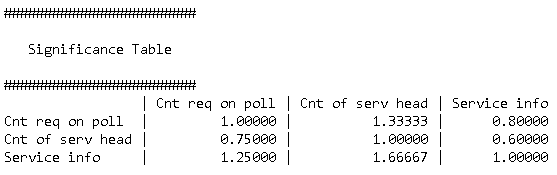
\includegraphics[width=1\linewidth]{my_folder/images/ATransferData1}
	\caption{Таблица значимости}
	\label{fig:atransferdata1}
\end{figure}

\begin{figure}
	\centering
	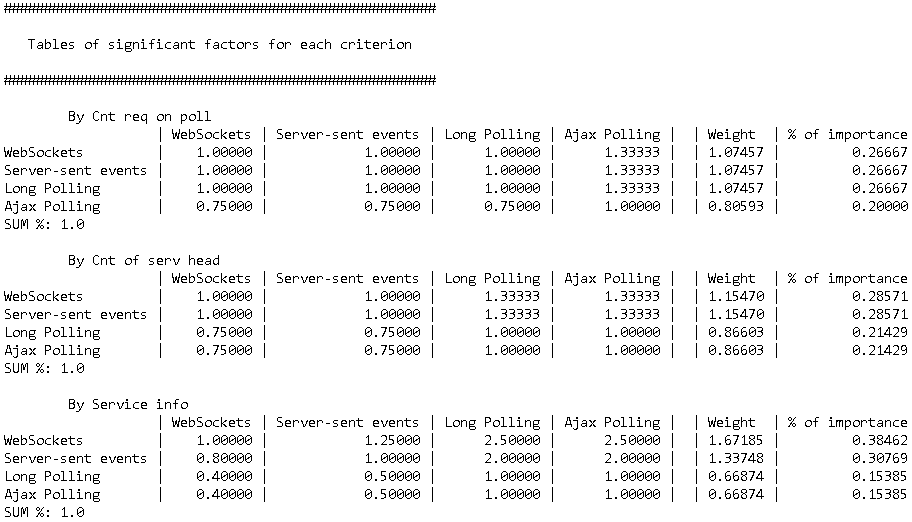
\includegraphics[scale=0.7, angle=270]{my_folder/images/ATransferData2}
	\caption{Таблицы значимых факторов для каждого критерия}
	\label{fig:atransferdata2}
\end{figure}

\begin{figure}
	\centering
	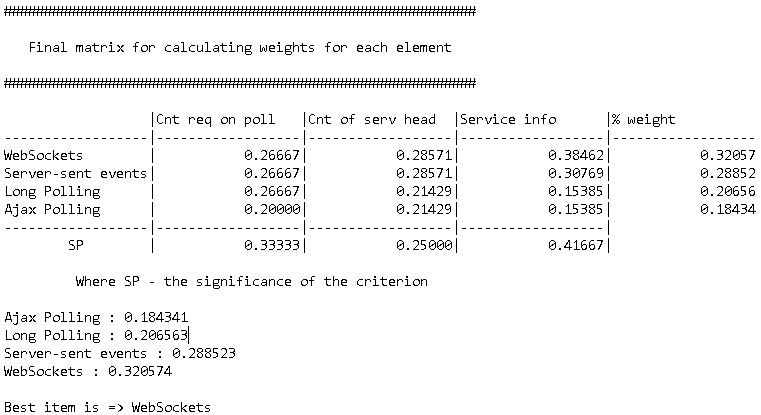
\includegraphics[width=1\linewidth]{my_folder/images/ATransferData3}
	\caption{Результируюящя таблица}
	\label{fig:atransferdata3}
\end{figure}			 	 % Приложение 2


\end{document} % конец документа


%%% Удачной защиты ВКР! - Good luck on the thesis defense!
%%
%%% Поддержать проект
%%
%% Запросы на добавление / изменение просим писать на следующей странице:
%% https://github.com/ParkhomenkoV/SPbPU-student-thesis-template/issues
%%
%% Список пожеланий в файле шаблона <<TO-DO-list.tex>>
%%
%% Благодарности просим указывать в виде 
%%
%% 1. Добавление <<Звезды>> проекту https://github.com/ParkhomenkoV/SPbPU-student-thesis-template/stargazers
%%
%% 2. Добавления <<Сердечка>> и репоста проекта в социальных сетях:
%%		https://vk.com/latex_polytech 
%%		https://www.fb.com/groups/latex.polytech
%%

%%% Support project
%%
%% Requests on adding / modifications is better to be publishen on the following web-page:
%% https://github.com/ParkhomenkoV/SPbPU-student-thesis-template/issues
%%
%% Wishlist is in the template's file called <<TO-DO-list.tex>>
%%
%% Acknowledgements are better to be done in the form of 
%%
%% 1. Adding <<Star>> to the project https://github.com/ParkhomenkoV/SPbPU-student-thesis-template/stargazers
%%
%% 2. Adding <<Likes>> and Project repost in the social networks:
%%		https://vk.com/latex_polytech 
%%		https://www.fb.com/groups/latex.polytech
%% 

% Check list при передаче ВКР:
% - Количество страниц в Задании 2. Если нет, то комментирование последней строки в my_task.tex
% - Зачистка всех вспомогательных файлов (Clear auxilary files) и компиляция ВКР не менее 3х раз